\documentclass[12pt, dvipsnames]{report}

\usepackage{amsmath}
\usepackage{algorithm}
%\usepackage{algorithmic}
\usepackage[noend]{algpseudocode}

\usepackage{amsmath}
\usepackage{amssymb}
\usepackage{amsthm}
\usepackage{amsopn}

\usepackage{kpfonts}

\usepackage{graphicx}

% Probably don't need this on notes anymore
%\usepackage{kbordermatrix}

% Standard tool for drawing diagrams.
\usepackage{tikz}
\usepackage{tkz-berge}
\usepackage{tikz-cd}
\usepackage{tkz-graph}

\usepackage{comment}

%
\usepackage{multicol}

%
\usepackage{framed}

%
\usepackage{mathtools}

%
\usepackage{float}

%
\usepackage{subfig}

%
\usepackage{wrapfig}

%
\let\savewideparen\wideparen
\let\wideparen\relax
\usepackage{mathabx}
\let\wideparen\savewideparen

% Used for generating `enlightening quotes'
\usepackage{epigraph}

% Forget what this is used for :P
\usepackage[utf8]{inputenc}

% Used for generating quotes.
\usepackage{csquotes}

% Allows what to generate links inside
% generated pdf files
\usepackage{hyperref}

% Allows one to customize theorem
% environments in mathematical proofs.
\usepackage{thmtools}

% Gives access to a proof
\usepackage{lplfitch}

% I forget what this is for.
\usepackage{accents}

% A package for drawing simple trees,
% as a substitute for unnesacary TIKZ code
\usepackage{qtree}

% Enables sequent calculus proofs
\usepackage{ebproof}

% For braket notation
\usepackage{braket}

% To change line spacing when using mathematical notations which require some height!
\usepackage{setspace}

%\usepackage[dvipsnames]{xcolor}

\usepackage{float}

% For block commenting
\usepackage{comment}




\setlength\epigraphwidth{8cm}

\usetikzlibrary{arrows, petri, topaths, decorations.markings}

% So you can do calculations in coordinate specifications
\usetikzlibrary{calc}
\usetikzlibrary{angles}

\theoremstyle{plain}
\newtheorem{theorem}{Theorem}[chapter]
\newtheorem{axiom}{Axiom}
\newtheorem{lemma}[theorem]{Lemma}
\newtheorem{corollary}[theorem]{Corollary}
\newtheorem{prop}[theorem]{Proposition}
\newtheorem{exercise}{Exercise}[chapter]
\newtheorem{fact}{Fact}[chapter]

\newtheorem*{example}{Example}
\newtheorem*{proof*}{Proof}

\theoremstyle{remark}
\newtheorem*{exposition}{Exposition}
\newtheorem*{remark}{Remark}
\newtheorem*{remarks}{Remarks}

\theoremstyle{definition}
\newtheorem*{defi}{Definition}

\usepackage{hyperref}
\hypersetup{
    colorlinks = true,
    linkcolor = black,
}

\usepackage{textgreek}

\makeatletter
\renewcommand*\env@matrix[1][*\c@MaxMatrixCols c]{%
  \hskip -\arraycolsep
  \let\@ifnextchar\new@ifnextchar
  \array{#1}}
\makeatother

\renewcommand*\contentsname{\hfill Table Of Contents \hfill}

\newcommand{\optionalsection}[1]{\section[* #1]{(Important) #1}}
\newcommand{\deriv}[3]{\left. \frac{\partial #1}{\partial #2} \right|_{#3}} % partial derivative involving numerator and denominator.
\newcommand{\lcm}{\operatorname{lcm}}
\newcommand{\im}{\operatorname{im}}
\newcommand{\bint}{\mathbf{Z}}
\newcommand{\gen}[1]{\langle #1 \rangle}

\newcommand{\End}{\operatorname{End}}
\newcommand{\Mor}{\operatorname{Mor}}
\newcommand{\Id}{\operatorname{id}}
\newcommand{\visspace}{\text{\textvisiblespace}}
\newcommand{\Gal}{\text{Gal}}

\newcommand{\xor}{\oplus}
\newcommand{\ft}{\wedge}
\newcommand{\ift}{\vee}

\newcommand{\prob}{\mathbf{P}}
\newcommand{\expect}{\mathbf{E}}
\DeclareMathOperator{\Var}{\mathbf{V}}
\newcommand{\Ber}{\text{Ber}}
\newcommand{\Bin}{\text{Bin}}

%\newcommand{\widecheck}[1]{{#1}^{\ft}}

\DeclareMathOperator{\diam}{\text{diam}}

\DeclareMathOperator{\QQ}{\mathbf{Q}}
\DeclareMathOperator{\ZZ}{\mathbf{Z}}
\DeclareMathOperator{\RR}{\mathbf{R}}
\DeclareMathOperator{\HH}{\mathbf{H}}
\DeclareMathOperator{\CC}{\mathbf{C}}
\DeclareMathOperator{\AB}{\mathbf{A}}
\DeclareMathOperator{\PP}{\mathbf{P}}
\DeclareMathOperator{\MM}{\mathbf{M}}
\DeclareMathOperator{\VV}{\mathbf{V}}
\DeclareMathOperator{\TT}{\mathbf{T}}
\DeclareMathOperator{\LL}{\mathcal{L}}
\DeclareMathOperator{\EE}{\mathbf{E}}
\DeclareMathOperator{\NN}{\mathbf{N}}
\DeclareMathOperator{\DQ}{\mathcal{Q}}
\DeclareMathOperator{\IA}{\mathfrak{a}}
\DeclareMathOperator{\IB}{\mathfrak{b}}
\DeclareMathOperator{\IC}{\mathfrak{c}}
\DeclareMathOperator{\IP}{\mathfrak{p}}
\DeclareMathOperator{\IQ}{\mathfrak{q}}
\DeclareMathOperator{\IM}{\mathfrak{m}}
\DeclareMathOperator{\IN}{\mathfrak{n}}
\DeclareMathOperator{\IK}{\mathfrak{k}}
\DeclareMathOperator{\ord}{\text{ord}}
\DeclareMathOperator{\Ker}{\textsf{Ker}}
\DeclareMathOperator{\Coker}{\textsf{Coker}}
\DeclareMathOperator{\emphcoker}{\emph{coker}}
\DeclareMathOperator{\pp}{\partial}
\DeclareMathOperator{\tr}{\text{tr}}

\DeclareMathOperator{\supp}{\text{supp}}

\DeclareMathOperator{\codim}{\text{codim}}

\DeclareMathOperator{\minkdim}{\dim_{\mathbf{M}}}
\DeclareMathOperator{\hausdim}{\dim_{\mathbf{H}}}
\DeclareMathOperator{\lowminkdim}{\underline{\dim}_{\mathbf{M}}}
\DeclareMathOperator{\upminkdim}{\overline{\dim}_{\mathbf{M}}}
\DeclareMathOperator{\lhdim}{\underline{\dim}_{\mathbf{M}}}
\DeclareMathOperator{\lmbdim}{\underline{\dim}_{\mathbf{MB}}}
\DeclareMathOperator{\packdim}{\text{dim}_{\mathbf{P}}}
\DeclareMathOperator{\fordim}{\dim_{\mathbf{F}}}

\DeclareMathOperator*{\argmax}{arg\,max}
\DeclareMathOperator*{\argmin}{arg\,min}

\DeclareMathOperator{\ssm}{\smallsetminus}

\title{Algebraic Geometry}
\author{Jacob Denson}

\begin{document}

\pagenumbering{gobble}
\maketitle
\tableofcontents
\pagenumbering{arabic}

\part{Classical Algebraic Geometry}

\chapter{Affine Algebraic Sets}

\section{A Brief History of Algebraic Curves}

Classically, Euclidean geometry discusses the relations between lines, circles, and their intersections. The practical foundations for this were that the most reliable tools of the time, the compass and unmarked ruler, trivialized the precise constructions of these shapes. However, in the late 19th century, this geometry was proven insufficient for certain constructions. One cannot use a ruler and compass to split an arbitrary angle into three, nor construct a square with the same area as a given circle. The Greeks did not have the apparatus required to show that attempts of these impossible problems were doomed to fail, but they realized their ineptitude, and introduced more sophisticated tools to solve these problems. Menaechmus `doubled a cube` with the introduction of the parabola. Pappus used the hyperbola to trisect the angle. Thus the conic sections became a canonical part of Euclidean geometry.

Thanks to Descartes' analytical geometry, we can identify the Euclidean plane with coordinates: tuples of two numbers. Furthermore, lines, circles, and conic sections are then described as the {\it locus} of points satisfying some algebraic relationship between the coordinates. The circle is the set of points satisfying $X^2 + Y^2 = 1$, the hyperbola $X^2 - Y^2 = 1$, and the parabola $Y = X^2$. An \emph{algebraic plane curve} is a subset in the plane described as the locus of a polynomial equation. They are ubiquitous throughout geometry, and the techniques used to understand them formed the historical foundation for the study of algebraic geometry.

\begin{example}
    A \emph{cissoid} is a curve constructed from two curves $C_1$, $C_2$, and a pole $O$. It is obtained by taking lines through $O$ intersecting both $C_1$ and $C_2$ at points $P_1$ and $P_2$, and marking off the points $Q$ such that $OQ$ has the same length and orientation as $P_1P_2$. If we take $C_1$ to be a circle, $C_2$ a line tangent to the circle, and $O$ the point on the circle opposite the tangent line, we obtain the cissoid of Diocles, introduced to solve the problem of doubling a cube.
    %
    \begin{center}
    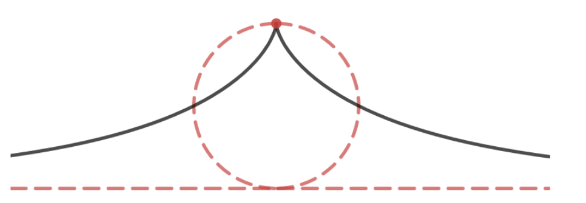
\includegraphics[width=0.7\textwidth]{CissoidDiocles}
    \end{center}
    %
    The name cissoid originates from the Greek \textkappa \textiota \textsigma \textsigma \textomikron \textepsilon \textiota \textdelta \texteta \textvarsigma, meaning `ivy shaped`, probably because of the singular, or cuspal points common in the curves, like in the cissoid of Diocles. We can also describe the cissoid of Diocles by letting a point $P$ range over all points on the circle, and then obtaining a point $Q$ by first reflecting $P$ across the line parallel to the fixed tangent bisecting the circle to obtain a point $P'$, and then intersecting the line $OP$ with the line through $P'$ parallel to the tangent. The easiest way to see why this is true is to look at the diagram below, and use similarity of triangles.
    %
    \begin{center}
        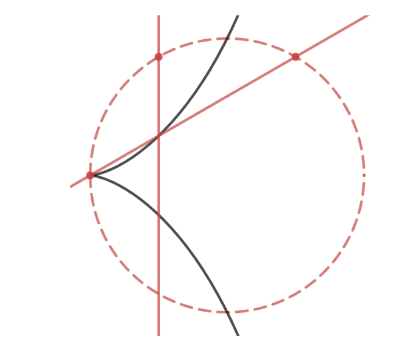
\includegraphics[width=0.4\textwidth]{CissoidDiocles2}
    \end{center}
    %
    If we consider a coordinate system in which $O$ lies at the origin, the circle is the unit circle with center $(1,0)$, and the tangent is the linear $X = 2$, then in polar coordinates, we may write the points on the circle as the solutions to the equation $r = 2 \sec \theta$, and the points on the tangent as solutions to $r = 2 \cos \theta$. The distance between the tangent line and the circle for a fixed angle $\theta$ is the difference in radii, which is just $2 \sec \theta - 2 \cos \theta$, and therefore the polar equation defining the cissoid of Diocles is
    %
    \[ r = 2(\sec t - \cos t) = \frac{2 - 2\cos^2 t}{\cos t} = \frac{2 \sin^2 t}{\cos t}\]
    %
    Since $X = r \cos t$, $Y = r \sin t$, and $r^2 = X^2 + Y^2$, in cartesian coordinates this equation becomes
    %
    \[ X = \frac{2Y}{X^2 + Y^2} \]
    %
    so the cissoid of Diocles is the locus of points defined by the polynomial equation $(X^2 + Y^2) X = 2Y^2$, and is therefore an algebraic planar curve.
\end{example}

\begin{example}
    Another construction of Diocles' cissoid was discovered by Newton. Consider a rigid right angled joint forced to pass through a point $O$, and another point $P$ lying on a line not passing through $O$, where the length of the joint from the bend to the point $P$ is fixed, but the length through $O$ is allowed to vary. As we move the point $P$ along the line, the joint slides back and forth through the point $O$. If we take the midpoints $Q$ between the point $P$ and the bend in the joint, then we obtain the cissoid of Diocles. We have expressed Diocles' cissoid as a \emph{conchoid}, which is constructed from a general point $O$ and curve by taking points on lines through $O$ lying at a fixed distance from the curve. In this case, the curve is a line, and the distance is half the distance between the point and the line.
%
    \begin{center}
        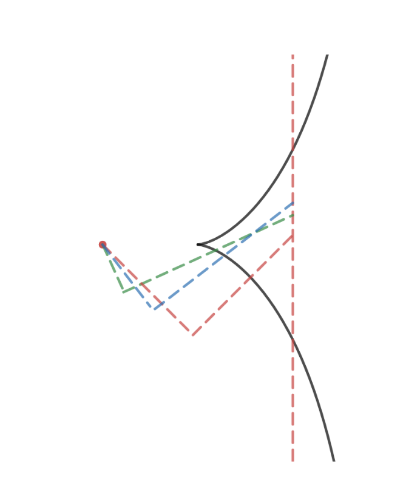
\includegraphics[width=0.4\textwidth]{ConchoidDiocles}
    \end{center}
%
    Suppose we choose a coordinate system in which $O = (-1,0)$, and the line over which $P$ varies is $X = 1$. If $Q$ has coordinates $(a,b)$, and $P$ has coordinates $(1,p)$, then the fact that $OQP$ is a right angle is equivalent to saying that $\langle O - Q, P - Q \rangle = 0$, which gives the equation $a^2 + b^2 = 1 + bp$. The condition that $PQ$ has length 2 is equivalent to the algebraic equation $a^2 + b^2 + p^2 = 3 + 2a + 2bp$, which, assuming the first equation is satisfied, is equivalent to $p^2 = 2 + 2a + bp$. Introducing the midpoint $(X,Y)$ of $PQ$, which is the point we want to exist in the first place, we find that
    %
    \[ 2X = a + 1\ \ \ \ 2Y = b + p \]
    %
    The first equation allows us to eliminate $a$ from the first two equations, and the second allows us to eliminate $b$. We obtain that the values of $X$ and $Y$ which lie on the shape are exactly those such that there exists a value $p$ such that $(2X - 1)^2 + (2Y - p)^2 = 1 + (2Y - p)p$ and $p^2 = 2 + 2(2X - 1) + (2Y - p)p$, which is simplified to the two equation $4X^2 + 4Y^2 + 2p^2 = 6pY + 4X$ and $p^2 = 2X + pY$. Substituting the second equation into the first gives $X^2 + Y^2 = pY$, and substituting this equation back into the second, after multiplying the equation by $Y^2$ on both sides gives $(X^2 + Y^2)^2 = (2X + X^2 + Y^2)Y^2$, which can be simplified to $(X^2 + Y^2)X = 2Y^2$, so this constructing describes exactly the cissoid of Diocles.
    %
    \begin{center}
        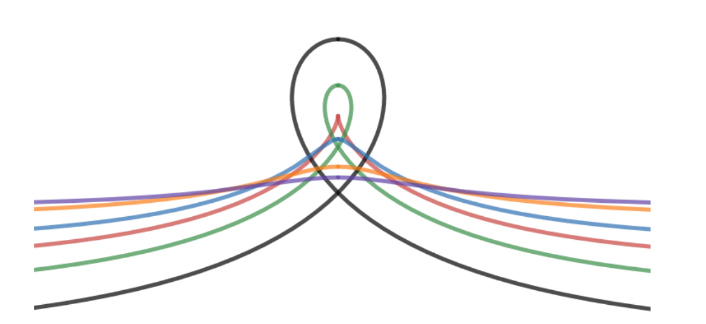
\includegraphics[width=0.8\textwidth]{ConchoidDiocles2}
    \end{center}
    %
    The advantage of Newton's construction is that we can obtain a one-parameter family of conchoidal curves which are deformations of the cissoid of Diocles, by taking points on the joint lying at a different ratio than the midpoint. Indeed, if $X = ac + (1 - c)$ and $Y = cb + (1-c)p$, then provided that $c \neq 0$ we can still use the first equation to eliminate $a$, and use the second to  eliminate $b$, obtaining that
    %
    \[ X^2 + Y^2 + 2(c-1)X + p(c-2)Y + (1 - c)p^2 = 2c - 1\ \ \ \ \  p^2 = 2X + pY + 4c - 2 \]
    %
    Substituting the second equation into the first gives $pY = X^2 + Y^2 - 4c^2 + 4c - 1$, and substituting the equation back into the second once multiplying by $Y$ on both sides of the equation gives
    %
    \[ X^4 + X^2Y^2  - 2XY^2 - 2(2c-1)^2X^2 + (1 - 4c^2)Y^2 = -16c^4 + 32c^3 - 24c^2 + 8c - 1 \]
    %
    These are quartic curves, which for $c < 1/2$ have a `loop' singularity, and are smooth for $c > 1/2$. The polynomial equations defining the quartic conchoids of Diocles are quartic, but we can obtain similar behavior in the cubic sense. These are the conchoids of de Sluze, described by the equation $(X-1)(X^2 + Y^2) = aX^2$, which is equal to the conchoid of Diocles when $a = -1$.
    %
    \begin{center}
        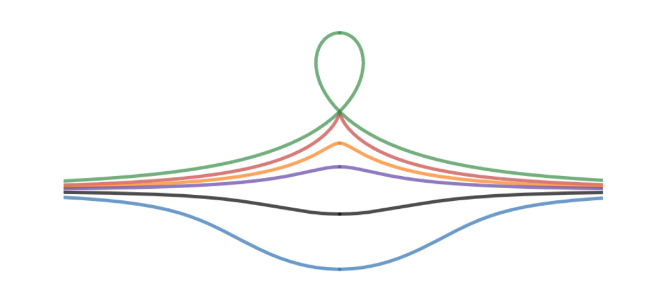
\includegraphics[width=0.7\textwidth]{ConchoidDesluze}
    \end{center}
\end{example}

\begin{example}
    Another example of an algebraic plane curve is the conchoid of D\"{u}rer, obtained by taking a pair of perpendicular lines intersecting at a point $O$, considering points $Q$ and $R$ moving on these lines such that the sum of the distances from $O$ to $Q$ and $O$ to $R$ is constant, and then taking the point on $QR$ at a fixed distance from $Q$. If we take the perpendicular lines as the $X$ and $Y$ axis, with $O$ the origin, take $b$ as the sum of distances, and take $a$ as the distance from $Q$, then each point $(X,Y)$ lies on the curve if, first, it lies on a line $PQ$, where $Q = (x,0)$ and $P = (0,y)$, where $yX + xY = xy$, such that $x + y = b$, and $(X - x)^2 + Y^2 = a^2$. We can eliminate $y$ from the equation since we can write $y = b -x$, so that $(b-x)X + xY = x(b-x)$. For a fixed $X$ and $Y$, this equation is quadratic in $x$, which can be rewritten as $x^2 + bX = x(b + X - Y)$. The equation $(X - x)^2 + Y^2 = a^2$ gives $x^2 = a^2 - Y^2 - X^2 + 2xX$, hence $a^2 - Y^2 - X^2 + bX = x(b - X - Y)$, which gives $(b - X - Y)x = a^2 - Y^2 - X^2 + bX$. Finally, we obtain the constraints on $X$ and $Y$ by multiplying the equation $(b - x)X + xY = x(b - x)$ on both sides by $(b - X - Y)^2$ allows us to eliminate the remaining values of $x$, which can be rearranged to give the equation
    %
    \[ 2y^2(x^2 + y^2) + (b^2 - 3a^2)y^2 + 2a^2b(x + y) + a^2(a^2 - b^2) = a^2x^2 + 2by^2(x + y) \]
    %
    so the curve is a quartic curve. For $b = 0$, the curve becomes a pair of lines together with a circle, and for $a = 0$, we obtain two coincident straight lines.
    %
%    \begin{center}
%        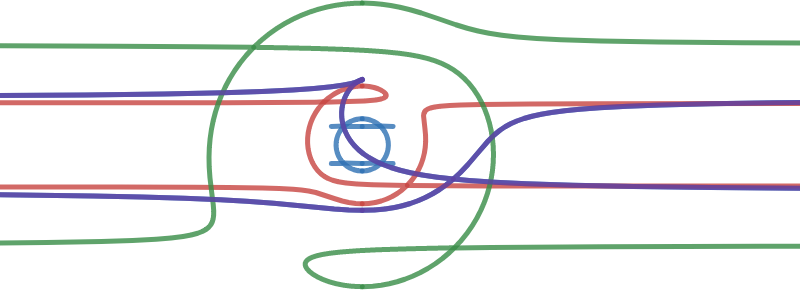
\includegraphics[width=0.7\textwidth]{algebraicGeometryConchoidDurer}
%    \end{center}
\end{example}

\begin{example}
    The conchoid of Nicomedes is obtained by fixing a point $P$, and letting $Q$ vary over a line not containing $P$. For each $Q$, the conchoid consists of the points on the line $PQ$ at a fixed distance away from $Q$. If we choose a coordinate system where $P$ lies at $(a,0)$, $Q$ lies at $(b,0)$, and the distance parameter is $b$, then the equation describing the conchoid is $(X - a)^2(X^2 + Y^2) = b^2X^2$. The conchoids appear to take three different forms depending on the relation between the distance between $P$ and the line, and the distance defining the conchoid. If $P$ is further away than the distance defining the conchoid, then we obtain two smooth curves. If $P$ is closer than the distance defining the conchoid, then the conchoid appears to `swing' around $P$, meeting $P$ in two intersection points. If the distance to $P$ is equal to the distance defining the conchoid, then we obtain a `cusp' at $P$, where the curve appears to swing towards $P$, and then swing out giving a sharp point. An interesting feature of the conchoid is that the time for an object to reach the `bottom' of the conchoid under the influence of gravity is independent of its original starting position. Another interesting feature of the conchoid is that it consists of two separate components lying on either side of the line $X = a$, with the line as an asymptote.
\end{example}

\begin{example}
    Just as we can obtain the conic sections by intersecting a cone with a parabola, the spiric sections of perseus are obtained by intersecting a plane with a torus. The general form of an equation describing a spiric section is of the form $(X^2 + Y^2)^2 = dX^2 + eY^2 + f$. A particular family of spiric sections include the Cassini curves. These can be constructed by taking two focal points $P$ and $Q$, and considering the locus of points such that the product of the distances to $P$ and to $Q$ are a fixed quantity. If we fix the focal points at $(-1,0)$ and $(1,0)$, then an equation for the Cassini curve is $(X^2 + Y^2)^2 - 2(X^2 - Y^2) + 1 = a^4$, where $a$ is the distance parameter to the curve. Cassini was an astronomer who believed the sun rotated around the earth according to these curves. The curves are smooth, except if we let the distance $a$ be equal to $1$, in which case the point $(0,0)$ is singular since the curve intersects twice here. This curve is the lemniscate of Bernoulli, described by the equation $(X^2 + Y^2)^2 = 2(X^2 - Y^2)$.
\end{example}

\begin{example}
    The folium of Descartes is the algebraic curve defined by the equation $X^3 + Y^3 = 3XY$. It's claim to fame is that was the curve that lead to the problem of implicit differentiation. In 1638, Descartes challenged Fermat to find the tangent line to the curve at any point on the circle, and with some primordial techniques of the calculus, Fermat was able to derive the tangent line at an arbitrary point.
\end{example}

\begin{example}
    If we consider a circle lying on the outside of a circle, and we fix a point on the circle as it rotates around the circle, then provided that the circumference of the outer circle is a rational multiple of the circumference of the inner circle, we obtain an algebraic curve known as an epicycloid, and the rational multiple determined the period of rotation of the circle. If the inner circle has radius $R$, and the outer circle radius $r$, then we have a parameterization given by
    %
    \[ \left( (r + R) \cos t - r \cos \left(\frac{r + R}{r}t \right), (r + R) \sin t - r \sin \left( \frac{r + R}{r}t \right) \right) \]



    If the circumference of the inner circle is equal to the circumference of the outer circle, the outer circle completes a single rotation before returning to its original location, and this curve is known as a cardoid, because it has a single cusp which looks like a heart. If the outer circle has half the circumference as the inner circle, the outer circle rotates twice before returning to its original position, and we obtain a function with a single cusp, and we call this shape a nephroid, since the shape looks like a kidney. Similarly, the hypocycloids are obtained by revolving a circle along the interior of the circle. If we revolve the outer circle around the inner circle, we obtain a pericycloid. If we fix a general point on these circles, we obtain the trochoids.
\end{example}

Algebraic curves are a rich source of geometric problems. For this reason, they inspired the general theory of algebraic geometry. Here are some questions we can ask about algebraic curves:
%
\begin{itemize}
    \item Is it possible to parameterize an algebraic curve's points by a rational function of a single argument? We call such curves \emph{rational curves}. This is more difficult than it seems. For instance, the algebraic curve $Y^2 = X^2 + X^3$ has a rational parameterization. For each value of $t$, the line $Y = tX$ intersects the curve in a single position outside of the origin, because the solutions are given by nonzero values of $X$ such that $(tX)^2 = X^2 + X^3$, so that $(t^2 - 1)X^2 = X^3$, so $X = t^2 - 1$, $Y = t^3 - t$ gives the unique point off the origin on the line $Y = tX$. But since every point on $Y^2 = X^2 + X^3$ lies on some line through the origin, we find that $(t^2 - 1, t^3 - t)$ gives a parameterization of the curve. This is not just a novel problem, because if we wish to perform an integration
    %
    \[ \int \varphi \left(x, \sqrt{x^2 + x^3} \right) dx\ \ \ \ \ \int \varphi \left( x, - \sqrt{x^2 + x^3} \right) dx \]
    %
    where $\varphi$ is a rational function in two variables, then we know that the substitution $x = t^2 - 1$ gives $\sqrt{x^2 + x^3} = t(t^2 - 1)$, so we are reduced to performing the integration
    %
    \[ \int \varphi(t^2 - 1, t(t^2 - 1)) 2t\; dt \]
    %
    Thus the antiderivative of every rational function of $x$ and $\sqrt{x^2 + x^3}$ is expressible in elementary terms. On the other hand, the cubic curve $Y^2 = X^3 + 1$ is not parameterized by a rational function of a single variable, and this is closely related to the fact that the integral
    %
    \[ \int \frac{dx}{\sqrt{x^3 + 1}} \]
    %
    is not expressible in terms of elementary functions.

    \item Another reason to study rational curves is to determine the points on a curve with rational coefficients. For instance, we can consider the rational solutions to the curve $Y^2 = X^2 + X^3$. We know that for each $t \in \mathbf{Q}$, $(t^2 - 1, t(t^2 - 1))$ gives a point on the curve with rational coordinates. Conversely, if $(t^2 - 1, t(t^2 - 1))$ is a rational coordinate, then $t^2$ is a rational number, and provided that $t^2 - 1 \neq 0$, we conclude that $t$ is also a rational number. On the other hand, if $t^2 - 1 = 0$, then $t = \pm 1$ is obviously rational. Thus we can obtain all rational points on the curve by taking the function of a single rational number. Fermat's last theorem asks us to determine whether the equation $X^n + Y^n = Z^n$ has any integer solutions for $n > 2$, which is equivalent to the existence of rational solutions to the equation $X^n + Y^n = 1$, so the problem is very closely related to problems about algebraic curves.

    \item It is an important problem in algebraic geometry to classify curves. The classical way to identify two curves is if they are equal to one another once we change our coordinate system. One invariant of this process is the \emph{degree} of the curve, that is, the degree of the polynomial defining the curve. Thus we have degree one curves, which are lines, the degree two curves, the conics, which are after discounting degenerate solutions, classified into parabolas, hyperbolas, and ellipses. But the cubics give a whole new world; Newton gave a classification of the cubic curves into 72 families; Pl\"{u}cker into a more systematic 219 class system.

    To simplify the situation, we can `weaken' the classification we use. If we view algebraic curves as lying in projective space rather than affine space, and identify curves by changing projective coordinates rather than affine coordinates, then the ellipse, hyperbola, and parabola are all identified as the same family of curves. We can imagine that the classification of cubics is also simplified considerably. Another way to simplify this situation is to identify two curves which are `intrinsically the same', in the sense that we can map one curve onto another by a coordinate map given by polynomial equations, whose inverse can also be specified by polynomial equations. We call these isomorphisms \emph{regular maps}. If we identify curves by rational functions rather than polynomials, we obtain the \emph{birational maps} between curves. The curves birationally equivalent to a line are exactly the rational curves. These are the basic notions leading to the intrinsic theory of algebraic geometry.
\end{itemize}
%
Polynomials, being a rather restricted class of functions, defined a class of fairly well behaved curves. Aside from the class of smooth curves, however, they possess certain irregularities.
%
\begin{itemize}
    \item Algebraic curves can have \emph{singular points} where the curve is no longer `smooth'. If an algebraic curve is defined with respect to a polynomial $f$, and $(\nabla f)(p) \neq 0$ where $f(p) = 0$, then we can locally describe one coordinate on the curve as a function of another curve, so the curve is smooth. But it is entirely possible for $(\nabla f)(p)$ to vanish, in which case the algebraic curve no longer behaves smoothly. One reason this can occur is if the algebraic curve has a \emph{node}, which occurs if $p$ is the intersection point of two smooth branches of the curve. Another reason is if the function rapidly changes direction, in which case we have a \emph{cusp}. Unless we restrict the class of algebraic curves we are considering to the \emph{non-singular} curves, then there is no way to avoid this issue, and we must face singular points head on.

    \item The zero sets of some polynomials do not have `curve-like' solutions at all. For instance, the equation $X^2 + Y^2 = 0$ has only a single solution $(0,0)$, so given our present definition we have to agree that $\{ (0,0) \}$ is an algebraic curve. This annoyance disappears when we study algebraic plane curves over the complex numbers, whose algebraic completeness means that $X^2 + Y^2$ factors into $(X + iY)(X - iY)$, so the solution set is the union of two planes, known as \emph{complex lines}, through the origin, so the solution set behaves locally like a two dimensional space. A two-dimensional space is `one-dimensional' over the complex numbers, so the solution set over the complex numbers behaves like a \emph{complex curve}. This is where the theory of Riemann surfaces enter the picture, and we find an interesting interplay between analytic and algebraic viewpoints.
\end{itemize}
%
On the other hand, being an essentially algebraic object, most of the basic techniques can be formalized to study algebraic curves over any field. In general, we shall assume some field $k$ is fixed, and we then study the $n$ dimensional affine space $\mathbf{A}^n$ over the field $k$, which can be identified with the space $k^n$ of $n$ tuples of field elements after a coordinate system is fixed. $\mathbf{A}^1$ is referred to colloquially as the affine line, and $\mathbf{A}^2$ as the affine plane. On a first glance, geometric intuition appears to break down over the finite fields, or other abstract fields, but surprisingly, the arguments which justify certain solutions to algebraic geometry over the complex numbers generalize to most other fields. The only specialization we may need to introduce is to assume that $k$ is an algebraically closed field, but we can always obtain results over any field by embedding a field in its algebraic closure. Often, this even gives further geometric insight enabling us to prove relations entirely in the original field.

\begin{example}
    Here is an example where working over the complex numbers enables us to prove relations about geometry in the Euclidean plane. If $P$ is a point outside a circle, it is the intersection point of two tangent lines on the circle, and we define the {\it polar line} to be the line through these two points on the circle. If the point $(x,y)$ lies on the circle, the tangent passing through it is described by the equation $xX + yY = 1$, and if $P = (a,b)$, then we must find $x$ and $y$ such that $ax + by = 1$, and $x^2 + y^2 = 1$. Multiplying this equation by $a^2$ and subtituting $1 - by$ for $ax$, we conclude
    %
    \[ (a^2 + b^2)y^2 - 2by + (1 - a^2) = 0 \]
    %
    The discriminant of this equation is $4a^2(a^2 + b^2 - 1)$, and so the equation has two distinct solutions provided that $a^2 + b^2 > 1$. But if $0 < a^2 + b^2 < 1$, the discriminant is negative, and we therefore get two complex points instead of two real valued points, but since the equations describing these points were real, the coordinates of these points must be complex conjugates of one another. If we let one of these points be $(x,y)$, then the equation describing the line between the two points is
    %
    \[ (\overline{x} - x)(Y - y) = (X - x)(\overline{y} - y) \]
    %
    Simplifying, the line is described by the equation
    %
    \[ \text{Im}(x) Y - \text{Im}(y) X = \text{Im}(x) \text{Re}(y) - \text{Im}(y) \text{Re}(x) \]
    %
    a purely real line, which can still be interpreted in a polar sense. Geometrically, it is the locus of all points whose polar line passes through $P$. Thus we are lead to a construction which would not have seemed so simple would we have restricted ourselves to real space, and it leads naturally to an exploration of the theory of inversive geometry.
\end{example}

We shall return to the study of algebraic plane curves after we introduce some general tools from the framework of algebraic geometry. However, algebraic curves offer a nice source of nontrivial examples with which to try out the general tools of algebraic geometry. Moreover, they are historically the reason algebraic geometry was studied in the first place, and the aid us understand modern teminology from the historical development of the subject.

\section{Affine Varieties}

Given a polynomial $f \in k[X_1, \dots, X_n]$, we can consider the set of its zeroes $V(f) = \{ p \in \mathbf{A}^n : f(p) = 0 \}$, which is the \emph{hypersurface} defined by $f$, a generalization of planar curves to higher dimensions. However, in higher dimensional space, it is also natural consider the geometric object formed from the common zeroes of two polynomials $V(f,g) = V(f) \cap V(g)$. More generally, given a set $S$ of polynomials, we can consider the set $V(S)$, which consists of the points forming the set of common zeroes of all polynomials in $S$. These zero sets are called \emph{affine varieties}, and they are the main object of study in algebraic geometry. The class of affine varieties is interesting from the point of view of Euclidean geometry, because it is invariant under affine transformations, and we have seen many of the interesting shapes in Euclidean geometry can be identified with certain varieties, through the tools of analytic geometry. If $T$ is an affine transformation on $\mathbf{A}^n$, and if we define the endomorphism $T^*$ on $k[X_1, \dots, X_n]$ by letting $T^*f = f \circ T$, then $T^{-1}(V(\mathfrak{a})) = V(T^* \mathfrak{a})$, so the two shapes are essentially equal. It is easy to prove that $T^*$ preserves the degree of polynomials, which is one of the reasons why the degree of polynomials is an {\it isomorphism-invariant} property of algebraic curves, when our isomorphisms are obtained by affine transformations.

\begin{theorem}
    A hypersurface $\Sigma$ in $\mathbf{A}^n$ specified by a polynomial of degree $d$ either contains a line, or intersects it in at most $d$ places.
\end{theorem}
\begin{proof}
    Let $\Sigma$ be specified by a polynomial $f(X) = \sum a_\alpha X^\alpha$. The points of the surface on a line $X = X_0 + t Y$ are in one to one correspondence with the zeroes of the polynomial $g(t) = \sum a_\alpha (X_0 + t Y)^\alpha$, which has degree at most $d$. In particular, unless $g = 0$, in which case $\Sigma$ contains the line, or $g$ intersects the line in at most $d$ places.
\end{proof}

As a consequence of this theorem, we see that affine curves in the plane cannot exhibit periodic phenomena along a line. In particular, we see that the points $(x,y)$ in $\mathbf{A}^2$ satisfying the equation $y = \sin(x)$ cannot form a planar curve, because the curve intersects the $x$ axis infinitely often. Similarily, the set of points $(z,w)$ in the complex affine plane satisfying $|z|^2 + |w|^2 = 1$ do not form an affine variety, since the intersection of the complex sphere with the $z$ axis is a circle, which has infinitely many points.

There are some elementary observations we can make on the construction $V(S)$ from a set of polynomials $S$, which open the floodworks to reducing geometric problems on varieties to the ring theory of $k[X_1, \dots, X_n]$.
%
\begin{itemize}
    \item If $S \subset T$, then $V(T) \subset V(S)$.

    \item If $\mathfrak{a}$ is the smallest ideal containing $S$, then $V(S) = V(\mathfrak{a})$, so every affine variety can be described as the common zeroes of some ideal.

    \item If we have a family $\{ \mathfrak{a}_\alpha \}$ of ideals, then $V(\bigoplus \mathfrak{a}_\alpha) = \bigcap V(\mathfrak{a}_\alpha)$, so the intersection of an arbitrary family of varieties forms a variety.

    \item For any two polynomials $f$ and $g$, $V(fg) = V(f) \cup V(g)$. More generally, if $\mathfrak{a}$ and $\mathfrak{b}$ are ideals, then $V(\mathfrak{a}\mathfrak{b}) = V(\mathfrak{a}) \cup V(\mathfrak{b})$, so finite unions of varieties are varieties.

    \item $V(0) = \mathbf{A}^n$, $V(1) = \emptyset$, and for any $a \in k^n$, $V(X_1-a_1,\dots,X_n - a_n)$ is just the singleton set $\{ a \}$. It follows from the last point that finite point sets are varieties.
\end{itemize}
%
The schema of algebraic geometry is that the geometric properties of a variety are completely summarized in the algebraic structure of the ring of functions $k[X_1, \dots, X_n]$ acting on the variety. This correspondence is strengthened tenfold when the field $k$ is algebraically closed, as proved by Hilbert's Nullstellensatz theorem. We now explore some properties of this ring, which give geometric properties of the class of affine varieties.

Another nice feature of the class of planar algebraic curves is that it takes on a combinatorial nature not found in the space of all smooth curves, a space which can only be effectively analyzed using analytical methods. This is because even if a variety is specified by an ideal $\mathfrak{a}$ consisting of infinitely many polynomials, the ideal $\mathfrak{a}$ is still generated by finitely many polynomials, and so the variety is cut out by a finite set of polynomials.

\begin{example}
    The varieties of $\mathbf{A}^1$ are exactly the finite point sets (other than the trivial variety $V(0) = \mathbf{A}^1$. First, note that since $k[X]$ is a principal ideal domain, we may assume we are considering the varieties of the form $V(f)$ for some particular polynomial $f(X) = \sum a_i X^i$. We know that $f(a) = 0$ if and only if $X - a$ is one of the prime factors of $f$. Since $f$ decomposes into finitely many prime factors, it follows that $V(f)$ can consist of at most $\text{deg}(f)$ points, a finite quantity. Thus the theory of one dimensional algebraic geometry is essentially trivial. This example shows that the countable union of affine varieties need not be a variety, because the countable union of finite sets need not be finite.
\end{example}

\begin{example}
    If $k$ is finite, all subsets of $\mathbf{A}^n$ are varieties, because all subsets of $\mathbf{A}^n$ are finite subsets. In order to study subsets of finite fields using polynomials, we need to place more specifications on the ideals we use in $\mathbf{A}^n$ so that interesting subsets of $\mathbf{A}^n$ are carved out.
\end{example}

\begin{prop}
    If $f$ is a non constant polynomial over an algebraically closed field, $\mathbf{A}^n - V(f)$ contains infinitely many points for $n \geq 1$, and $V(f)$ contains infinitely many points for $n \geq 2$.
\end{prop}
\begin{proof}
    First, recall that every algebraically closed field $k$ must have infinitely many points, because if $k$ only contains $a_1, \dots, a_n$, we are unable to factor $(X - a_1) \dots (X - a_n) + 1$ into linear factors. It follows that $\mathbf{A}^1 - V(f)$ is infinite for any polynomial $f \in k[X]$, because $V(f)$ is finite. Given any polynomial $f \in k[X_1, \dots, X_n]$, there is a line in $\mathbf{A}^n$ upon which $f$ is not identically zero (for otherwise $f$ is equal to zero everywhere), and reducing our argument to the one dimensional case, we see that infinitely many points on this line cannot be zeroes of $f$. Arguing similarly, given any $f \in k[X_1, \dots, X_n]$, there is a plane upon which $f$ does not vanish uniformly, and so we must show that any nonconstant $f(X,Y) = \sum a_{ij} X^i Y^j$ in the plane has infinitely many zeroes. Without loss of generality, we may assume that $V(f)$ does not contain the origin. Assuming this, the intersections of $V(f)$ with the lines through the origin break $V(f)$ into disjoint classes of points, and provided we can show infinitely many of these classes are nonempty, we can conclude that $V(f) = \emptyset$. For any line through the origin of the form $Y = aX$, the polynomial takes the form $f(X,aX) = \sum a_{ij} a^j X^{i+j}$, and we know this polynomial has a zero unless it is constant, and if this occurs, then for any $1 \leq m < \infty$, $\sum a_{(m-k)k} a^k = 0$. Each of these are polynomials in $k[a]$, and at least one of these polynomials is nonzero, so we conclude there can only be finitely many values $a$ such that the line $Y = aX$ does not have an intersection with $V(f)$, and it follows that $V(f)$ is infinite, because $k$ is infinite.
\end{proof}

If $X$ is any set, then we shall let $I(X)$ be the subset of $k[X_1, \dots, X_n]$ of polynomials which vanish over $X$. The set forms an ideal, and it is clear that in the case where $X = V(S)$, the ideal contains all elements of $S$, hence all elements of $\mathfrak{a}$. The generation of an ideal $I(X)$ from a set $X$ is dual to the notion of generating a set $V(\mathfrak{a})$ from an ideal $\mathfrak{a}$. We make a few elementary observations about this operator.
%
\begin{itemize}
    \item It is clear that if $X \subset Y$, then $I(Y) \subset I(X)$.
    \item $I(\emptyset) = k[X_1, \dots, X_n]$, and $I(\mathbf{A}^n) = (0)$.
    \item $S \subset I(V(S))$ for any subset $S$ of polynomials, and $X \subset V(I(X))$.
    \item Combining the last two points, it follows that $V(I(V(S))) = V(S)$, because $V(S) \subset V(I(V(S)))$ follows from the second point of the last bullet, and $V(I(V(S)) \subset V(S)$ follows because $S \subset I(V(S))$. Similarly, we can argue that $I(V(I(X))) = I(X)$. Thus if $X$ is an algebraic set, then $V(I(X)) = X$, and if $\mathfrak{a}$ is an ideal equal to $I(X)$ for some set $X$, then $I(V(\mathfrak{a})) = \mathfrak{a}$.
    \item If $f^n \in I(X)$, then $f^n(p) = 0$ for all $p \in X$, which implies $f(p) = 0$ because $k$ is an integral domain, so that $f \in I(X)$. This means exactly that $I(X)$ is a {\it radical ideal} (a radical ideal $\mathfrak{a}$ is an ideal such that if $x^n \in \mathfrak{a}$ is in $x$. The smallest radical ideal containing some ideal $\mathfrak{a}$ is denoted $\text{Rad}(\mathfrak{a})$.
\end{itemize}

\begin{prop}
    For any two algebraic sets $V$ and $W$, $I(V) = I(W)$ if and only if $V = W$.
\end{prop}
\begin{proof}
    This follows because $V(I(V)) = V$, and $V(I(W)) = W$, so if $I(V) = I(W)$, then $V = V(I(V)) = V(I(W)) = W$.
\end{proof}

This simple proposition is clearly not true if $V$ and $W$ are not algebraic sets, hinting that the class of varieties is well separated by polynomial functions. For instance, if $Y$ is the closure of some open set $X$ in $\mathbf{C}^n$, then $I(X) = I(Y)$, because polynomials are continuous so if they vanish on $X$, they certainly vanish on $Y$. The fact also shows that there is a certain correspondence between algebraic sets and radical ideals. If two algebraic sets determine the same radical ideal, they are equal. We will soon see that if we are working over an algebraically closed field, and $\mathfrak{a}$, $\mathfrak{b}$ are radical ideals, then $V(\mathfrak{a}) = V(\mathfrak{b})$ only if $\mathfrak{a} = \mathfrak{b}$, so there is a one two one correspondence between radical ideals and algebraic sets. This constitutes the theory of Hilbert's nullstellensatz, which we will come back to later in this chapter.

\begin{corollary}
    If $V$ is an algebraic set in $\mathbf{A}^n$, and $p \not \in V$, then there is a polynomial $f$ which vanishes on $V$, but with $f(p) = 1$.
\end{corollary}
\begin{proof}
    Since $V \neq V \cup \{ p \}$, and $V$ and $V \cup \{ p \}$ are both algebraic sets, $I(V) \neq I(V \cup \{ p \})$, and since $I(V) \supset I(V \cup \{ p \})$, there must be a polynomial $f$ which vanishes on $V$, but with $f(p) \neq 0$. It follows by normalizing that we can assume $f(p) = 1$.
\end{proof}

Similarly, by taking an algebraic set $V$, and $n$ points $p_1, \dots, p_n \not \in V$, we may apply this theorem to find polynomials $f_1, \dots, f_n \in I(V)$ with $f_i(p_j) = \delta_{ij}$. By considering linear combinations of the $f_i$, for any $a_{ij} \in k$, we can find $f_1, \dots, f_n \in I(V)$ with $f_i(p_j) = a_{ij}$. This shows the space of polynomials which vanish over $V$ has enough degrees of freedom to specify values on a finite set of points.

\section{Reducibility}

An algebraic variety $V$ is said to be \emph{reducible} if it can be written as the union of two proper algebraic subsets. Otherwise, we say $V$ is \emph{irreducible}. Ring theory allows us to characterize this criterion in terms of the ideal generating the ideal.

\begin{prop}
    A variety $V$ is irreducible if and only if $I(V)$ is prime.
\end{prop}
\begin{proof}
    Suppose that $I(V)$ is not prime, so $fg \in I(V)$, whereas $f \not \in I(V)$, $g \not \in I(V)$. It follows that $f$ cannot be a scalar multiple of $g$, because $I(V)$ is a radical ideal. The fact that $f \not \in I(V)$ and $g \not \in I(V)$ means that $f$ and $g$ do not vanish on $V$, so $V(f, I(V))$ and $V(g, I(V))$ are proper subsets of $V$. But $V(f, I(V)) \cup V(g, I(V)) = V(fg, I(V)) = V(I(V)) = V$, so $V$ is reducible. Conversely, if $V = W \cup U$, where $W$ and $U$ are proper algebraic subsets of $V$, then $I(V)$ is a proper subset of both $I(W)$ and $I(U)$, so we may select $f$ vanishing on $W$, but not on $V$, and $g$ vanishing on $U$, but not on all of $V$. This means that $fg$ vanishes on $W \cup U = V$. Thus we have found $f,g \not \in I(V)$, but with $fg \in I(V)$, so $I(V)$ cannot be prime.
\end{proof}

\begin{example}
    The parabola $V(Y - X^2)$ is an irreducible variety over an infinite field. First, we must justify that $I(V(Y - X^2)) = (Y - X^2)$. If $f(X,Y) \in k[X,Y]$ is a polynomial, then we may apply the division algorithm, viewing $k[X,Y]$ as the one dimension polynomial ring $k[X][Y]$ with coefficients in $k[X]$, to obtain that $f(X,Y) = g(X,Y) (Y - X^2) + h(X)$. If $f(x,x^2) = 0$ for all $x \in k$, then $h(x) = 0$ for all $x \in k$, so if we are working over an infinite field we conclude that $h = 0$, and therefore $f$ is divisible by $Y - X^2$. Now we prove that $(Y - X^2)$ is prime. Since $k[X,Y]$ is a unique factorization domain, it suffices to show that $Y - X^2$ is an irreducible polynomial. If $Y - X^2$ is the product of two polynomials, write these two polynomials as $Yf(X) + g(X)$ and $h(X)$ (if there are more $Y$'s in the factorization, they clearly cannot multiply to $Y - X^2$). Then $f$ is monic. But now $(Yf + g)(h) = Yfh + gh$, so $fh = 1$, implying that $h$ is a unit.
\end{example}

As in most of mathematics, irreducible varieties have a nice theory, and we can use this theory to understand the varieties obtainable from the union of irreducible varieties. The idea is simple. If a variety $V$ is not irreducible, then we can break it apart into two proper algebraic subsets $V_1 \cup W_1$. If $V_1$ is not irreducible, we can break it apart into two proper subsets $V_2 \cup W_2$. If this process is guaranteed to terminate at some point (so that $V_n$ is eventually irreducible), we can recursively break apart varieties into irreducible varieties. The ring theoretic property we need to employ here is the fact that $k[X_1, \dots, X_n]$ is Noetherian.

\begin{lemma}
    If $I$ is an ideal of a Noetherian ring, then out of the set of prime ideals containing $I$, there are only finitely many minimal ones.
\end{lemma}
\begin{proof}
    If there was a counterexample to this lemma, there would certainly be a maximal counterexample $I$. The ideal $I$ cannot be prime, because then there would only be a single minimal prime ideal containin $I$. Thus there is $x$ and $y$ such that $xy \in I$, but $x, y \not \in I$. Thus $(x,I)$ and $(y,I)$ are ideals bigger than $I$, and so counterexamples to the theorem. Thus there are only finitely many minimal prime ideals in $(x,I)$ and $(y,I)$. But if $P$ is a prime ideal of $I$, then $xy \in P$, so either $x \in P$, or $y \in P$, so $(x,I) \subset P$ or $(y,I) \subset P$. Thus a minimal prime ideal in $I$ must be a minimal prime ideal in $(x,I)$ or $(y,I)$, which is a contradiction to the fact that there are infinitely many of them.
\end{proof}

\begin{theorem}
    Every variety is the unique finite union of irreducible varieties, with no variety including the other, known as the {\it irreducible components} of the variety.
\end{theorem}
\begin{proof}
    If $V$ is a variety, there are only finitely many minimal prime ideals containing $I(V)$, and thus there are only finitely many maximal irreducible varieties contained in $V$. Now if $V$ can be written as the union of two families of irreducible varieties $V_1, \dots, V_N$ and $W_1, \dots, W_M$, then $V_n = \bigcup (V_n \cap W_m)$, so either $V_n \cap W_m = \emptyset$ or $V_n \cap W_m = V_n$, which implies $V_n \subset W_m$ for some $m$. Performing the same process in reverse gives $W_m \subset V_{n'}$ for some $n$, and obviously $n = n'$. By matching up elements of the decomposition, we conclude that the decomposition is unique.
\end{proof}

\begin{example}
    Consider the variety $V(Y^4 - X^2, Y^4 - X^2Y^2 + XY^2 - X^3)$ in $\mathbf{C}^2$. Since $Y^4 - X^2 = (Y^2 - X)(Y^2 + X)$, we find
    %
    \begin{align*}
        Y^4 - X^2Y^2 + XY^2 - X^3 &= (Y + iX)(Y - iX)(Y-X)(Y+X)
    \end{align*}
    %
    Considering the zeroes which satisfy these equations on a case by case basis, we find that the variety is just a set of discrete points, each an irreducible factor of the decomposition of the variety.
\end{example}

\begin{example}
    The polynomial $Y^2 + X^2(X-1)^2$ is irreducible over $\mathbf{R}[X,Y]$, but factors into $(Y + iX(X-1))(Y - iX(X-1))$ over $\mathbf{C}[X,Y]$. The consequence is that even though $Y^2 + X^2(X-1)^2$ is an irreducible polynomial, the variety it generates is not irreducible, consisting of the two points $(0,0)$ and $(1,0)$. This is a consequence of the fact that over the real numbers,
    %
    \[ I(V(Y^2 + X^2(X-1)^2) = (Y,X(X-1)) \neq (Y^2 + X^2(X - 1)^2) \]
    %
    is not a prime ideal.
\end{example}

\section{Classification of Planar Algebraic Sets}

It an interesting task to classify the algebraic subsets of $\mathbf{A}^2$, because it is the first nontrivial family of algebraic sets. Whereas the algebraic subsets of $\mathbf{A}^1$ are trivial, the plane contains numerous infinite families of varieties, such as parabolas, ellipses, hyperbolas, and elliptic curves. We begin with a simple observation.

\begin{theorem}
    If two polynomials $f,g \in k[X,Y]$ are relatively prime, then $V(f,g)$ consists of finitely many points.
\end{theorem}
\begin{proof}
    If $f(X,Y)$ and $g(X,Y)$ have no common factor over $k[X,Y]$, then by the Gauss lemma they also have no common factor over $k(X)[Y]$, and because $k(X)[Y]$ is a Euclidean domain, we may write $af + bg = 1$ for some $a,b \in k(X)[Y]$. If $a(X,Y) = \sum a_i(X)Y^i$ and $b(X,Y) = \sum b_i(X) Y^i$, then we may find a nonzero $c \in k[X]$ such that $ca, cb \in k[X,Y]$. This implies that $(ac)f + (bc)g = c$. It follows that for any $x$ for which there exists $y$ with $f(x,y) = g(x,y) = 0$, $c(x) = 0$. Since $c$ has only finitely many roots, we conclude that $f(x,y)$ and $g(x,y)$ equal zero at only finitely many values of $x$. By symmetry, they can also only simultaneously be zero at finitely many values of $y$.
\end{proof}

A consequence of this is that we can classify the `dimension' of an algebraic variety in the plane in a very algebraic way. Given a variety $V$, we consider the largest possible chain of nonempty irreducible varieties $V \supset V_0 \supsetneq V_1 \supsetneq \dots V_n$. If $V$ is a planar curve, then we must have $n \leq 1$, because any proper irreducible variety contained in an irreducible planar curve must be a singleton by the above theorem. Over an algebraically closed field, we can set $n = 1$ because every planar curve is nonempty. The finite point sets can only have $n \leq 0$. The only planar variety where we can set $n = 2$ is the entire affine plane. Thus the dimensions of the underlying varieties are characterized by the largest chain of irreducible varieties they contain. Later on, we will take this as the definition of the dimension of a variety.

\begin{corollary}
    If $f(X,Y)$ is irreducible, and $V(f)$ is infinite, then $I(V(f)) = (f)$, and $V(f)$ is irreducible.
\end{corollary}
\begin{proof}
    If $g \in I(V(f))$, then $V(f,g) = V(f)$ is infinite, so $f$ and $g$ must have a common factor, hence $f$ must divide $g$ since $f$ is irreducible. We conclude that $I(V(f))$ consists only of multiples of $f$.
\end{proof}

\begin{corollary}
    The irreducible algebraic planar sets over an infinite field are exactly $\mathbf{A}^2$, $\emptyset$, singletons, and irreducible plane curves $V(f)$, where $f$ is irreducible and $V(f)$ is infinite.
\end{corollary}
\begin{proof}
    It is obvious that $\{ p \}$ is an irreducible set, as is $\emptyset$. Since $k$ is an infinite field, it is also obvious that $\mathbf{A}^2$ is irreducible, since $I(\mathbf{A}^2) = (0)$ is irreducible. Any other irreducible algebraic set must be of the form $V(f)$ for some irreducible polynomial $f$, and these are the irreducible planar curves provided $V(f)$ is infinite, by the last lemma.
\end{proof}

\begin{corollary}
    If we are working over an algebraically closed field, and $f$ is not irreducible, so we can write $f = f_1^{n_1} \dots f_m^{n_m}$ where each $f_i$ is irreducible, then the irreducible components of $V(f)$ are exactly the $V(f_i)$. We find that $I(V(f)) = (f_1, \dots, f_n)$.
\end{corollary}
\begin{proof}
    It is clear that
    %
    \[ V(f) = V((f_1^{n_1}) \dots (f_m^{n_m})) = \bigcup V(f_i^{n_i}) = \bigcup V(f_i) \]
    %
    and that each $f_i$ is irreducible. Since our field is algebraically closed, each $V(f_i)$ is infinite, If $V(f_i) \subset V(f_j)$, then $V(f_i,f_j) = V(f_j)$, and since $V(f_j)$ is infinite, this implies that $f_j$ divides $f_i$, which is impossible. Thus the $V(f_i)$ really are the decomposition of $V(f)$.
\end{proof}

\begin{example}
    Over the real numbers, $X^2 + Y^2 + 1$ is irreducible, yet no points in the real plane satisfy the equation $X^2 + Y^2 = 1$, so $I(V(X^2 + Y^2 + 1)) = \mathbf{R}[X,Y]$, which is not equal to $(X^2 + Y^2 + 1)$. Conversely, $X^2 + Y^2 + 1$ is also irreducible over the complex numbers, but the solution set to the polynomial forms an irreducible complex curve.
\end{example}

This is the first of many algebraic deficiencies of non algebraically closed fields, which is one of the reasons we will soon switch to studying algebraically closed fields.

\begin{example}
    As another example, note that the variety over the real numbers corresponding to $Y^2 - XY - X^2Y + X^3 = (Y - X)(Y - X^2)$ is the union of the line $Y = X$ and the parabola $Y = X^2$, and this is the decomposition into irreducible elements. The same is true for the decomposition over the complex numbers.
\end{example}

\begin{example}
    $Y^2 - X(X^2 - 1)$ is an irreducible polynomial, and its solution set is infinite, so $V(Y^2 - X(X^2 - 1))$ is an irreducible variety both over the real and complex numbers. In the topology of the Euclidean plane, $V(Y^2 - X(X^2 - 1))$ is disconnected though, the union of a shape isomorphic to the disjoint union of a circle and a line. On the other hand, over the complex numbers the solution set of $Y^2 - X(X^2 - 1)$ is a connected set which can be written as the union of the two branches of the function $Y = \sqrt{X(X^2 - 1)}$, and since the Riemann surface corresponding to the square root operation is homeomorphic to $\mathbf{C}$, the solution set of this polynomial is also homeomorphic to $\mathbf{C}$ -- it has three singularities at $X \in \{ -1, 0, 1 \}$, and the solution set behaves like a cone around these solution sets.
\end{example}

\begin{example}
    Over the real numbers, $X^3 + X - X^2Y - Y = (X-Y)(X^2 + 1)$ is just the line $X = Y$, and hence $V(X^3 + X - X^2Y - Y)$ is irreducible. However, over the complex numbers, $X$ is the union of the three lines $X = Y$, $X = i$, and $X = -i$, and is therefore reducible.
\end{example}

\section{The Nullstellensatz}

We have seen the duality between affine varieties and radical ideals over the ring $k[X_1, \dots, X_n]$. Over algebraically closed fields, the correspondence between radical ideals and algebraic sets becomes exact. This is the content of Hilbert's Nullstellensatz theorem. A precursor to the Nullstellensatz, known as Study's lemma will suffice for the study of planar algebraic curves.

\begin{theorem}[Study]
    If $f$ and $g$ are polynomials in the affine plane over an algebraically closed field with $V(f) \subset V(g)$, and $f$ is irreducible, then $f$ divides $g$.
\end{theorem}
\begin{proof}
    If $f$ did not divide $g$, then $f$ and $g$ would be relatively prime, so $V(f,g)$ would consist of finitely many points. But $V(f)$ is contained in $V(f,g)$, which is impossible.
\end{proof}

In terms of ideals, Study's lemma implies that if $f$ is a irreducible polynomials, then $I(V(f)) = (f)$. Hilbert's first generalizes this result to saying that if $f$ is an irreducible polynomial in any dimension, then $I(V(f)) = (f)$, and more generally, if $f$ vanishes on a variety $V(\mathfrak{a})$, then $f^n \in \mathfrak{a}$ for some integer $n$.

\begin{lemma}[Weak Nullstellensatz]
    If $k$ is an algebraically closed field, and if $\mathfrak{a}$ is a proper ideal of $k[X_1, \dots, X_n]$, then $V(\mathfrak{a}) \neq \emptyset$.
\end{lemma}
\begin{proof}
    We shall actually prove that if $\mathfrak{a}$ is a maximal ideal, then $V(\mathfrak{a})$ is a set containing a single point. Since we may always extend every ideal to a maximal ideal, this will prove the proposition. So we take $\mathfrak{a}$ to be any maximal ideal. Then $k[X_1, \dots, X_n]/\mathfrak{a} = L$ is a field, which can be viewed as a field extension of $k$ because we can embed $k$ as the set of constant polynomials in $k[X_1, \dots, X_n]$, and we then compose with the quotient homomorphism to obtain a map into $L$. We write $x_i \in L$ for the element of the field corresponding to $X_i$. If we know that the embedding of $k$ in $L$ gives an isomorphism between the two fields, then for each $x_i$ there is $a_i \in k$ with $x_i - a_i \in \mathfrak{a}$. But $(X_1 - a_1, \dots, X_n - a_n)$ is a maximal ideal in $k[X_1, \dots, X_n]$, hence $\mathfrak{a} = (X_1 - a_1, \dots, X_n - a_n)$. Now we can conclude that $V(\mathfrak{a}) = \{ (a_1, \dots, a_n) \}$.
\end{proof}

An important thing to note about this proof of the weak Nullstellensatz is that it implies that the maximal ideals of $k[X_1, \dots, X_n]$ are in one to one correspondence with the points of $\mathbf{A}^n$. The fact that maximal ideals are in one to one correspondence with points in space occurs in other context of mathematics, for instance, in the ring theory of $C(X)$, where $X$ is Hausdorff and locally compact. This point of view is often so useful that, when we study general rings $A$, we consider the set of maximal ideals of $A$ as points in a space, and then viewing elements of $A$ as functions on this space. This idea reoccurs later in our study of the local rings attached to varieties, and with the generalization of varieties to schemes.

To finish off the proof of the weak Nullstellensatz, it suffices to prove that if $k$ is an algebraically closed field, then for every field $L$, if there is a surjective homomorphism from $k[X_1, \dots, X_n]$ to a field extension $L$ of $k$ fixing elements of $k$, then $k = L$. This is an easy consequence of Zariski's lemma, which we prove now.

\begin{lemma}
    If $k[x_1, \dots, x_n]$ is a field, then it is a finite extension of $k$.
\end{lemma}
\begin{proof}
    We prove this by induction on $n$. For $n = 1$, this is a classical argument in Galois theory. To continue the induction, suppose we have proved the theorem for all fields of the form $k[x_1, \dots, x_m]$, where $m < n$. We may then apply induction to $k[x_1, \dots, x_n] = k(x_1)[x_2, \dots, x_n]$ to conclude that $k[x_1, x_2, \dots, x_n]$ is a finite extension of $k(x_1)$. But this means that there are rational functions $a_0(x_1), \dots, a_{N-1}(x_1)$ of $x_1$ such that $x_1^N = \sum a_n(x_1) x_1^n$. But now there exists a polynomial $f \in k[x_1]$, such that $f(x_1) a_n(x_1) \in k[x_1]$ for all $n$, and we find
    %
    \[ x_1^N = \sum f(x_1) a_n(x_1) x_1^n \]
    %
    Which means $x_1$ is algebraic over $k$, and therefore a finite extension of $k$. This completes the proof.
\end{proof}

Since all finite extensions of a field are algebraic over that field, we conclude that if $k$ is algebraically closed, then every field of the form $k[x_1, \dots, x_n]$ is an algebraic extension of $k$, and therefore $k[x_1, \dots, x_n] = k$. This finishes our proof of the weak nullstellensatz. We now consider the extension to the full nullstellensatz.

\begin{theorem}
    If $\mathfrak{a}$ is an ideal in $k[X_1, \dots, X_n]$, where $k$ is algebraically closed, then $I(V(\mathfrak{a})) = \text{Rad}(\mathfrak{a})$, where $\text{Rad}(\mathfrak{a})$ is the set of all $f$ for which there exists $n$ with $f^n \in \mathfrak{a}$.
\end{theorem}
\begin{proof}
    We may assume that $\mathfrak{a}$ is generated by finitely many polynomials, so $\mathfrak{a} = (f_1, \dots, f_m)$.  Concretely, the nullstellensatz then says that if $g$ vanishes on the common nullset of the $f_1, \dots, f_m$, then $g^N = \sum h_kf_k$ for some $h_m \in k[X_1, \dots, X_n]$. Suppose that $g \in I(V(\mathfrak{a}))$. Consider the ideal $\mathfrak{b} = (f_1, \dots, f_m, X_{n+1}g - 1) \subset k[X_1, \dots, X_{n+1}]$. Then $V(\mathfrak{b}) = \emptyset$, since if $f_1(x) = \dots = f_n(x) = 0$, then $g(x) = 0$, so $x_{n+1}g(x) - 1 = -1$. The weak nullstellensatz implies that there are $a_k \in k[X_1, \dots, X_{n+1}]$ such that
    %
    \[ \sum a_k f_k + b (X_{n+1}g - 1) = 1 \]
    %
    Introducing $Y = 1/X_{n+1}$, we may multiply the equation by $Y^N$ for a large enough $N$ to find that
    %
    \[ Y^N = \sum Y^N a_k f_k + b Y^{N-1}(g - Y) \]
    %
    Where the $Y$ in $Y^N a_k$  can $Y^{N-1}b$ can be used to cancel out all instances of $X_{n+1}$. Setting $Y = g$ gives the required equation over $k[X_1, \dots, X_n]$.
\end{proof}

\begin{corollary}
    There is a one to one correspondence between radical ideals and algebraic sets in affine space over an algebraically closed field.
\end{corollary}

\begin{corollary}
    If $\mathfrak{a}$ is a prime ideal, then it is also a radical non total ideal, so $V(\mathfrak{a}) \neq \emptyset$ is an irreducible algebraic variety, and there is a one to one correspondence with such prime ideals and irreducible varieties. The maximal ideals correspond to points in $\mathbf{A}^n$.
\end{corollary}

\begin{example}
    $V(Y^2 - X(X-1)(X-\lambda))$ is an irreducible planar curve in $\mathbf{A}^2$ in any algebraically closed field, because $Y^2 - X(X-1)(X-\lambda)$ is an irreducible polynomial. If the polynomial does factor, it factors as $(Y + f(X))(Y - f(X))$ where $-f(X)^2 = X(X-1)(X-\lambda)$, but then this equation has no solution because $X(X-1)(X-\lambda)$ isn't a square of a polynomial in $k[X]$, which is a unique factorization domain.
\end{example}

\begin{corollary}
    If $f \in k[X_1, \dots, X_n]$ has a decomposition as $f_1^{n_1} \dots f_m^{n_m}$, where $k$ is algebraically closed, then $V(f) = V(f_1 \dots f_n) = \bigcup V(f_i)$ is the decomposition of $f$ into its irreducible factors. There is a one to one correspondence (up to scalar multiples) between irreducible hyperplanes and irreducible polynomials.
\end{corollary}

It is clear that if $k$ is not an algebraically closed field, then the weak nullstellensatz cannot hold, because in one dimension, the weak nullstellensatz is exactly the condition that gives that $k$ is an algebraically closed field. Since $k[X]$ is a principal ideal domain, the theorem states that if $(f) \neq k[X]$, then $V(f) \neq 0$, which means that if $f$ is a non constant polynomial, then $f$ has a root.  The reason we work over algebraically closed fields is so that we have enough points on our algebraic curves to ensure a correspondence between ideals and polynomials. From now on, the fact that a field is algebraically closed is so integral that, unless otherwise mentioned, all field we discuss in the sequel will be assumed algebraically closed.

%\begin{example}
%    If $q$ is a prime element of a unique factorization domain, then every prime ideal $\mathfrak{a} \subset (q)$ is either trivial or equal to $(p)$. To see this, assuming $\mathfrak{a} \neq (0)$, we find a nonzero $p_1^{n_1} \dots p_m^{n_m} q^k \in \mathfrak{a}$ minimizing $k + \sum n_i$. Then we must have $k > 0$, so $q(p_1^{n_1} \dots p_m^{n_m} q^{k-1}) \in \mathfrak{a}$, and because of our minimization, $p_1^{n_1} \dots p_m^{n_m} q^{k-1} \not \in \mathfrak{a}$, so $q \in \mathfrak{a}$. This implies that if $V$ is an irreducible hyperplane, there is no irreducible variety containing $V$, except for $\mathbf{A}^n$ itself.
%\end{example}

%\begin{example}
%    Sometimes, we have to be a bit clever to determine if an ideal is reducible. Consider the ideal $(X^2 - Y^3,Y^2 - Z^3)$ in $k[X,Y,Z]$, where $k$ is algebraically closed. Consider the homomorphism $f$ from $k[X,Y,Z]$ to $k[T]$ preserving elements of $k$, and with $X \mapsto T^9$, $Y \mapsto T^6$, and $Z \mapsto T^4$. Then certainly $(X^2 - Y^3, Y^2 - Z^3)$ is contained in the kernel of $f$. But an arbitrary element of $k[X,Y,Z]/(X^2 - Y^3, Y^2 - Z^3)$ can be denoted $a + bX + cY + dXY$, with $a,b,c,d \in k[Z]$, and if $a = \sum a_i Z^i$, $b = \sum b_i Z^i$, $c = \sum c_i Z^i$, $d = \sum d_iZ^i$, then $a + bX + cY + dXY$ maps to
    %
%    \[ \sum a_i T^{4i} + \sum b_i T^{9 + 4i} + \sum c_i T^{6 + 4i} + \sum d_i T^{15 + 4i} \]
    %
%    and since the terms of each sum occur over different residues mod four, $f(a + bX + cY + dXY) = 0$ if and only if $a + bX + cY + dXY = 0$, hence the kernel of $f$ is exactly $(X^2 - Y^3, Y^2 - Z^3)$. Since $k[T]$ is an integral domain, this shows that $(X^2 - Y^3, Y^2 - Z^3)$ is prime, and therefore that $V(X^2 - Y^3, Y^2 - Z^3)$ is an irreducible variety. In other words, the parameterization $t \mapsto (t^9, t^6, t^4)$ maps $k$ onto our variety, and we will soon find that the image of an irreducible variety (in this case $k$) under a polynomial map is irreducible.
%\end{example}

\chapter{Intrinsic Properties of Algebraic Varieties}

\section{Coordinate Rings}

Often, to study the structure of some space $X$, we look at the space of functions on $X$ with some particular property reflecting the structure of $X$. For instance, if $X$ is a topological space, we look at the space of continuous functions. If $X$ is the complex plane, we look at the space of holomorphic functions. Normally, these spaces of functions will turn out to have an algebraic structure, like that of a ring, or an algebra over a field, and determining this algebraic structure up to isomorphism often classifies the spatial structure of $X$. Viewing an algebraic variety $V$ as a space, it seems difficult to think of which functions on $V$ are the natural ones. Studying continuous functions on $V$ can give us certain topological information about the variety, such as connectedness, compactness, and so on, but this information doesn't seem very related to the definition of $V$ in terms of $k[X_1, \dots, X_n]$. To make the connection between $V$ and $k[X_1, \dots, X_n]$, we make a decision that the natural functions `should' be the polynomial functions. We define the \emph{coordinate ring} of $V$, also known as the ring of \emph{regular functions} on $V$, denoted $k[V]$, to be the space of all functions which are the restriction of some polynomial function on $\mathbf{A}^n$. Algebraically, $k[V]$ forms an algebra over $k$, where the functions in $k[V]$ corresponding to elements of $k$ correspond to the constant functions on $V$. There is an alternate description of the coordinate ring which is more amenable to algebraic manipulation. The homomorphism from $k[X_1, \dots, X_n]$ to $k^{\mathbf{A}^n}$ obtained by mapping a polynomial to the function it defines can be composed with the restriction homomorphism from $k^{\mathbf{A}^n}$ to $k^V$, and the image of this composition is exactly $k[V]$. Applying the first isomorphism theorem, we find that $k[V]$ is isomorphic to $k[X_1, \dots, X_n]$ modulo the kernel of the homomorphism. This kernel is exactly the space of polynomials which vanish over $V$, which we previously denoted $I(V)$, so we find that $k[V]$ is isomorphic to $k[X_1, \dots, X_n]/I(V)$. This is useful for proving things formally about the coordinate ring of a variety.

\begin{example}
    If we are working over an infinite field, then the coordinate ring $k[\mathbf{A}^n]$ is equal to $k[X_1, \dots, X_n]$, because $I(\mathbf{A}^n) = 0$. This is well known in the univariate case. In general, if we have a nonzero polynomial $f(X_1, \dots, X_n,Y)$, then viewing the polynomial as a univariate polynomial in $Y$ with coefficients in $k(X_1, \dots, X_n)$, we conclude that there must be $y \in k$ with $f(X_1, \dots, X_n,y) \neq 0$, and by induction we conclude there are $x_1, \dots, x_n \in k$ with $f(x_1, \dots, x_n, y) \neq 0$. In particular, in an algebraically closed field this will always be true. On the other hand, if we are working over $GF(p^n)$, then every nonzero polynomial $f(X_1, \dots, X_n)$ with degree at most $p^n-1$ in each variable cannot vanish everywhere on $\mathbf{A}^n$, and the polynomials $\smash{X_n^{p^n-1} - 1}$ generate the ideal $I(\mathbf{A}^n)$.
\end{example}

A \emph{subvariety} of a variety $V$ is an algebraic set which occurs as a subset of $V$. The Nullstellensatz tells us that in an algebraically complete field, the subvarieties of $V$ are in one to one correspondence with the radical ideals containing $I(V)$. Applying the fourth isomorphism theorem, since the image of an ideal containing $I(V)$ is radical in $k[V]$ if and only if it is radical in $k[X_1,\dots,X_n]$, we find that the subvarieties of $V$ are in one to one correspondence with the radical ideals in $k[V]$. The points in $V$ are also in one to one correspondence with the maximal ideals containing $I(V)$. This is the first instance of the fact that we can view $V$ as an `algebraic space' independent of $\mathbf{A}^n$, in which `being a subvariety' corresponds to `being the locus of a radical ideal'. As another example, we note that if $I_V(W)$ is the ideal of functions in $k[V]$ vanishing on $W$, then $k[W]$ is isomorphic to $k[V]/I_V(W)$, so that quotienting by functions vanishing on a subvariety is a natural way to form a coordinate ring on a subvariety of an arbitrary variety, not just in an affine space. This is the first step in forming a `coordinate independent' way of defining varieties, which gives rise to modern algebraic geometry, wherein varieties need not lie in an ambient space.

\begin{prop}
    $V$ is finite if and only if $k[V]$ is finite dimensional as a vector space over $k$, and then it's dimension is the number of points in the variety.
\end{prop}
\begin{proof}
    If $p_1, \dots, p_n \in V$, we have seen that we can choose $f_1, \dots, f_n \in k[V]$ with $f_i(p_j) = \delta_{ij}$. Then $f_1, \dots, f_n$ are linearly independent in $k[V]$, because if $g = \sum \lambda_i f_i$ vanishes on $V$, then $g(p_j) = \sum \lambda_i f_i(p_j) = \lambda_j = 0$. In particular, if $V$ has infinitely many points, then $k[V]$ is an infinite dimensional vector space over $k$. Conversely, if $p_1, \dots, p_n$ are the only points in $V$, then $k[V]$ is spanned by the $f_i$, so $k[V]$ is finite dimensional.
\end{proof}

One can extend this result, using a technique which will become more useful later in our analysis of the ring theory of $k[X_1, \dots, X_n]$.

% MOVE TO MORE ADVANCED SECTION
\begin{lemma}
    Over an algebraically complete field, for any ideal $\mathfrak{a}$ of $k[X_1, \dots, X_n]$ such that $V(\mathfrak{a})$ is finite, $k[X_1, \dots, X_n]/\mathfrak{a}$ is finite dimensional over $k$. The number of points in $V(\mathfrak{a})$ is bounded by the dimension of the vector space.
\end{lemma}
\begin{proof}
    We have already seen this theorem if $\mathfrak{a}$ is a radical ideal, for then $I(V(\mathfrak{a})) = \mathfrak{a}$, and so $k[V]$ is isomorphic to $k[X_1, \dots, X_n]/\mathfrak{a}$. In general, $I(V(\mathfrak{a})) = \text{Rad}(\mathfrak{a})$, which we shall denote by $\mathfrak{b}$. Since $\mathfrak{b}$ is finitely generated, and each element of $\mathfrak{b}$ has a power which is in $\mathfrak{a}$, we conclude that there is an integer $n$ such that $\mathfrak{b}^n \subset \mathfrak{a} \subset \mathfrak{b}$. We then have the following sequence of surjective maps
    %
    \[ k[X_1, \dots, X_n]/\mathfrak{b}^n \to \dots \to k[X_1, \dots, X_n]/\mathfrak{b}^2 \to k[X_1, \dots, X_n]/\mathfrak{b} \]
    %
    The kernel of the map from $k[X_1, \dots, X_n]/\mathfrak{b}^{i+1}$ to $k[X_1, \dots, X-n]/\mathfrak{b}^i$ is $\mathfrak{b}^i/\mathfrak{b}^{i+1}$, which is finite dimensional, because if $\mathfrak{b}^i = (f_1, \dots, f_m)$, then the $f_i$ span $\mathfrak{b}^i/\mathfrak{b}^{i+1}$ because $f_if_j \in \mathfrak{b}^{i+1}$. Using the rank nullity theorem, we can use induction to prove that $k[X_1, \dots, X_n]/\mathfrak{b}^i$ is a finite dimensional vector space over $k$ for each $i$. The base case is that $k[X_1, \dots, X_n]/\mathfrak{b}$ is finite dimensional, and the general case is that
    %
    \[ \dim k[X_1, \dots, X_n]/\mathfrak{b}^{i+1} = \dim \mathfrak{b}^{i+1}/\mathfrak{b}^i + \dim k[X_1, \dots, X_n]/\mathfrak{b}^i \]
    %
    and the sum of two finite values is finite. Since $\mathfrak{b}^n \subset \mathfrak{a}$, we have a surjective map from $k[X_1, \dots, X_n]/\mathfrak{b}^n$ to $k[X_1, \dots, X_n]/\mathfrak{a}$, so $k[X_1, \dots, X_n]/\mathfrak{a}$ is finite dimensional.
\end{proof}

\begin{example}
    Consider the locus $V$ of the polynomials $Y^2 - X^2$ and $Y^2 + X^2$ over an algebraically closed field $k$. Since $(Y^2 - X^2, Y^2 + X^2) = (Y^2,X^2)$, the radical ideal of these polynomials is $(Y,X)$, and so $k[V] = k[X,Y]/(Y,X) \cong k$ is a one dimensional vector space over $k$. This makes sense, because $Y^2 - X^2 = (Y-X)(Y+X)$, so on $V$ we find $Y = X$ or $Y = -X$, and in either of these cases $Y^2 + X^2 = 0$ if and only if $X = Y = 0$.
\end{example}

Since the basic notion of algebraic geometry is the set of polynomials, the natural structure preserving maps between varieties should be those maps $f: V \to W$ should be those maps induced by polynomial maps. These are the \emph{regular maps}, also known as \emph{polynomial maps}. To be specific, a map $f: \mathbf{A}^n \to \mathbf{A}^m$ is regular if each coordinate map $f_1, \dots, f_m$ is induced by a polynomial function. The regular maps between two varieties $V$ and $W$ are then exactly those induced by a restriction of a polynomial map between $\mathbf{A}^n$ and $\mathbf{A}^m$. If $f: X \to Y$ is a map between two sets, then it induces a `pullback' map $f^*: k^Y \to k^X$ obtained by composition: $f^*g = g \circ f$. This map has many useful properties for our studies:
%
\begin{itemize}
    \item If $g: Y \to Z$ is another polynomial map, then $(g \circ f)^* = f^* \circ g^*$.
    \item If $f(X_0)$ is a subset of $Y_0$, then $f^*$ descends to a map from $k^{X_0}$ to $k^{Y_0}$, and this function respects the restriction homomorphisms.
    \item If $f: V \to W$ is a polynomial function, then $f^*$ maps functions in $k[W]$ to functions in $k[V]$. A polynomial map $f$ maps elements of $V$ into elements of $W$ if and only if $f^*$ maps $I(W)$ into $I(V)$.
    \item If $f: V \to W$ is a surjective map, then $f^*: k[W] \to k[V]$ is injective.
\end{itemize}
%
In fact, the algebra structure of $k[V]$ classifies $V$ as a variety, up to an application of a polynomial map.

\begin{prop}
    There is a one to one correspondence between regular maps between $V$ and $W$ and algebra homomorphisms from $k[W]$ to $k[V]$.
\end{prop}
\begin{proof}
    Given a homomorphism $T: k[W] \to k[V]$, we can define a polynomial map $f: V \to W$ by letting $f = (TX_1, \dots, TX_n)$, which is well defined over $V$. We claim that $Tg = g \circ f$ for all polynomials $g \in k[W]$. It is clear that the set of polynomials satisfying this equation include $1$ and $X_1, \dots, X_n$, and if $Tg_0 = g_0 \circ f$ and $Tg_1 = g_1 \circ f$, then $Tg_0g_1 = (g_0 \circ f)(g_1 \circ f) = (g_0g_1 \circ f)$. Since $1,X_1, \dots, X_n$ generate $k[V]$ as an algebra, we conclude that the equation is satisfied by all $g$. If $f$ is any polynomial map between two varieties, then $f^*(g) = g \circ f$, and the construction above reconstructs the function $f$, so we know there is a one to one correspondence.
\end{proof}

A polynomial map is a \emph{regular isomorphism} if it is bijection, and its inverse is also a polynomial map. Thus the intrinsic study of curves is characterized up to a regular isomorphism; the theory attempts to study the properties of varieties which are invariant under polynomial isomorphisms. We have argued that $k[V]$ is an isomorphism invariant of the variety $V$: two varieties $V$ and $W$ are isomorphic if and only if $k[V]$ and $k[W]$ are isomorphic. This means that the coordinate rings have sufficient expressive power, just like how $C(X)$ classifies $X$ when $X$ is a compact Hausdorff space, though this is much more difficult to prove. Since every finitely generated $k$ algebra $R$ which is {\it reduced} (if $x^n = 0$, $x = 0$) is the coordinate ring of some variety, the map $V \mapsto k[V]$ is an contravariant equivalence between the category of affine varieties and the category of reduced finitely generated $k$ algebras, when $k$ is algebraically closed. This is the reason the Nullstellensatz enables us to view geometric problems algebraically, and conversely, view algebraic problems geometrically.

\begin{prop}
    The image of an irreducible variety under a polynomial map is an irreducible variety.
\end{prop}
\begin{proof}
    Let $f: V \to W$ be a surjective polynomial map between two varieties, and suppose that $W$ is reducible, so that we may write $W = W_1 \cup W_2$. Then we have a decomposition of $V$ as $V_1 = f^{-1}(W_1)$ and $V_2 = f^{-1}(W_2)$, and $V_1, V_2 \neq V$ because otherwise this would imply that either $W_1 = W$ or $W_2 = W$.
\end{proof}

\begin{example}
    We have seen that $\{ (t,t^2,t^3): t \in k \}$ is an affine variety, because it is the locus of the polynomials $X^2 = Y$ and $X^3 = Z$. Another way to see this is to note that the variety is the image of the polynomial map from $\mathbf{A}^1$ to $\mathbf{A}^3$ defined by $t \mapsto (t,t^2,t^3)$. It is irreducible because it is the image of $\mathbf{A}^1$, which is an irreducible variety. What's more, the variety is isomorphic to $\mathbf{A}^1$, because the embedding has a polynomial inverse $(x,y,z) \mapsto x$.
\end{example}

\begin{example}
    The variety $V = V(XY - 1)$ is a curve {\it not} isomorphic to $\mathbf{A}^1$, because $k[V]$ is not isomorphic to $k[\mathbf{A}^1]$. To see this, we note that an isomorphism $f: k[\mathbf{A}^1] \to k[V]$ would induces a map on the group of units in each ring. But the units in $k[\mathbf{A}^1]$ are exactly the elements of $k - \{ 0 \}$, so the isomorphism, since it fixed $k$, allows us to conclude that $k[V]$ cannot have any other units than $k - \{ 0 \}$. But $X$ and $Y$ are both units in $k[V]$.
\end{example}

\begin{example}
    The locus $V$ of polynomials of the polynomials $XZ = Y^2$, $YZ = X^3$, and $Z^2 = X^2Y$ forms an irreducible variety over $\mathbf{C}$. Note that $Y^3 - X^4$ is in the ideal $(XZ - Y^2, YZ - X^3, Z^2 - X^2Y)$, and if $x,y \in k$ are picked such that $x^4 = y^3$, there is a unique $z \in k$ with $z = y^2/x = x^3/y$, unless $x = y = 0$. In this case, we conclude that $z = 0$ because $z^2 = x^2y$. Otherwise $z^2 = x^2y$ follows automatically because $z^2 = (y^2/x)(x^3/y)$. The polynomial map $t \mapsto (t^3,t^4,t^5)$ is therefore a surjective map from $\mathbf{A}^1$ onto $V$. For any $y \neq 0$, there are exactly four values of $t$ such that $t^4 = y$, and if $t$ is any solution then $it$, $-it$, and $-t$ form the other three solutions to the equation. Now if $x^4 = y^3$, then $x^4 = t^{12}$, and
    %
    \[ x^4 - t^{12} = (x - t^3)(x + t^3)(x - it^3)(x + it^3) \]
    %
    This implies that either $x = t^3$, $x = -t^3$, $x = it^3$, or $x = -it^3$. But by replacing $t$ with any of the other roots of the equation $t^4 = y$, we find that there is a unique value of $t$ such that $t^4 = y$ and $t^3 = x$. We conclude that the map $t \mapsto (t^3,t^4,t^5)$ is actually a bijection. The same argument essentially shows that $V$ is irreducible in any algebraically closed field: one must just take a bit of extra care when we are doing computations over a field of characteristic two.
\end{example}

\begin{example}
    For any $f \in k[V]$, where $V$ is some variety in $\mathbf{A}^n$, define the \emph{graph} $G(f)$ of $f$ to be the set of tuples $(a_1, \dots, a_{n+1}) \in \mathbf{A}^{n+1}$, where $(a_1, \dots, a_n) \in V$ and $a_{n+1} = f(a_1, \dots, a_n)$. $G(f)$ is isomorphic to $V$ under the projection map $(a_1, \dots, a_{n+1}) \mapsto (a_1, \dots, a_n)$, because for each $a_1, \dots, a_n$ the number $a_{n+1}$ is uniquely determined.
\end{example}

\begin{example}
    A bijective polynomial map need not be an isomorphism. Consider the polynomial map from $\mathbf{A}^1$ to $V(Y^2-X^3)$ defined by letting $f(t) = (t^3,t^2)$. Then $f$ is a bijection, but $f^*$ is not surjective, for it maps $X$ onto $t^3$, and $Y$ onto $t^2$, so $f^*(X^2) = f^*(Y^3)$, and the image of the map is therefore $k[t^3,t^2]$, which is a proper subset of $k[t]$.
\end{example}

As should be expected by a geometer, the isomorphisms of $\mathbf{A}^n$ contain the family of affine translations $x \mapsto Mx + b$, where $b \in \mathbf{A}^n$ and $GL_n(k)$. This is exactly the reason why we work in a space denoted by $\mathbf{A}^n$ rather than $k^n$, because the choice of isomorphisms mean that the particular choice of affine coordinates used to define varieties is of no real consequence to the geometry of varieties.

\begin{example}
    The affine subplanes of $\mathbf{A}^n$ are varieties known as \emph{linear subvarieties}. Any variety of the form $V(f_1, \dots, f_m)$, where each $f_i$ is of degree one, is a linear subvariety, in which case the subplane has dimension $n-m$. These subplanes are all isomorphic to $\mathbf{A}^{n-m}$. This can easily be seen by a projection, but can also be seen because a linear subvariety of dimension $n$ has coordinate ring isomorphic to $k[X_1, \dots, X_n]$.
\end{example}

\section{The Function Field of a Variety}

The ring $k[V]$ is an isomorphism invariant of $V$, but it is often difficult to work with. However, when $V$ is an irreducible variety, then $k[V]$ is an integral domain, because it is the quotient of $k[X_1, \dots, X_n]$ by a prime ideal. This means we can form the field of fractions, which we denote $k(V)$. The elements of $k(V)$ correspond to functions on $V$ defined except at certain singularity sets, known as the set of \emph{poles} of the function. Given $f \in k(V)$, we say $f$ is \emph{defined}, or \emph{regular} at $p \in V$ if we may write $f = g/h$, where $h(p) \neq 0$. Then $g(p)/h(p)$ is defined irrespective of the choice of $g$ and $h$, for if $g_0/h_0 = g_1/h_1$, then $h_1g_0 = h_0g_1$, and so $h_1(p)g_0(p) = h_0(p)g_1(p)$, hence $g_0(p)/g_1(p) = h_0(p)/h_1(p)$. Though $k(V)$ does not classify the isomorphism classes of algebraic varieties, an isomorphism between $k(V)$ and $k(W)$ still provides strong relations between the varieties $V$ and $W$, which are employed in their most basic form in the theory of rational curves. To consider this relation, we say that a set $X \subset V$ is \emph{Zariski dense} in $V$ if $V$ is the only subvariety of $V$ to contain all the points in $X$. This, in particular, implies that any function $f \in k[V]$ which vanishes on $X$ also vanishes on $V$, for the set of zeroes of $f$ form a subvariety of $V$ containing $X$. In a more modern context, this density can be interpreted as a topological density of a set in the \emph{Zariski topology} of a variety.

\begin{theorem}
    The $k$ homomorphisms $T: k(W) \to k(V)$ are in one to one correspondence with maps $f: V \to W$ definable by rational functions of the coordinates (so $f$ is really a partial map) whose image is Zariski dense in $W$.
\end{theorem}
\begin{proof}
    Suppose that $T: k(W) \to k(V)$ is a homomorphism. If $V \subset \mathbf{A}^n$ is definable in the coordinates $(X_1, \dots, X_n)$, and $W \subset \mathbf{A}^m$ is definable in the coordinate $(Y_1, \dots, Y_m)$, then let $T(Y_i) = f_i$. We claim that $(f_1, \dots, f_m)$ gives a surjective map from $V$ to $W$, where defined. Suppose that $y = (f_1(x), \dots, f_m(x))$ is not an element of $W$. Then there is $g \in I(W)$ with $g(y) = 1$. If $g(Y) = \sum a_\alpha Y^\alpha$, then since $g$ is equal to 0 in $k(W)$, we find that $T(g) = \sum a_\alpha f^\alpha = 0$ in $V$, so in particular $\sum a_\alpha f^\alpha(x) = g(y) = 0$, which is impossible. Similarly, if $y \in W$ was not in the Zariski closure of $f(V)$, then we could define a function $g \in k[W]$ vanishing on $f(V)$ but with $g(y) = 1$, and if $g = \sum a_\alpha Y^\alpha$, then $Tg = 0$, which implies $g = 0$, which is impossible. Conversely, if $f: V \to W$ is definable by rational functions in the coordinates whose image is Zariski dense in $W$, we can define $T: k[W] \to k(V)$ by letting $T(Y_i) = f_i$, because if $\sum a_\alpha Y^\alpha \in I(W)$, then $\sum a_\alpha f^\alpha \in I(V)$. If $T(\sum a_\alpha Y^\alpha) = \sum a_\alpha f^\alpha = 0 \in k(V)$, then $\sum a_\alpha Y^\alpha$ must vanish on $f(V)$, and this implies that $\sum a_\alpha Y^\alpha = 0$. This implies the map descends to a map from $k(V)$ to $k(W)$.
\end{proof}

The association of $f$ with $T$ is a contravariant functor from the category of algebraic varieties to the category of fields, so in particular, if we find $T^{-1}$ for some isomorphism $T$, then the rational functions $(f_1, \dots, f_m)$ corresponding to $T$ and the rational functions $(g_1, \dots, g_n)$ corresponding to $T^{-1}$ are inverse functions of one another, viewed as maps from $V$ to $W$. A map $f$ specifiable by rational functions with an inverse of the form $g$ is known as a \emph{birational} map. Again, we see that the Nullstellensatz implies the map $V \mapsto k(V)$ is a contravariant isofunctor from the category of irreducible varieties to the category of finite field extensions of $k$.

\begin{example}
    Let $f(X,Y)$ be an arbitrary irreducible quadratic polynomial in the plane, defining a planar curve $V$. We claim that $k(V)$ is isomorphic to $k(t)$, which is the function field of $k$, so in particular there is a birational map $g: k \to V$ parameterizing $V$. We can already guess such a birational map, since if $(x_0,y_0) \in V$, then there is at most one point in $V$ on any line through $(x_0,y_0)$, since $V$ is quadratic, implying we can parameterize the line by slope. If we define
    %
    \[ T = \frac{Y - y_0}{X - x_0} \in k(V) \]
    %
    In $k(V)$, we know $f(X, y_0 + T(X - x_0)) = f(X,Y) = 0$. This is a polynomial relation in $k(T)[X]$, and we know setting $X = x_0$ causes the polynomial to vanish, so $f(X, y_0 + T(X - x_0)) = (X - x_0)(a(T)X - b(T))$, for some $a,b \in k(T)$. Since $X - x_0 \neq 0$ in $k(V)$, $X = b(T)/a(T)$ on $V$. But this means $X \in k(T)$, and therefore all $Y = T(X - x_0) + y_0 \in k(T)$, so $k(V) = k(T)$. Finally, we know $k(T)$ is isomorphic to the field of rational functions in a single variable. An interesting application of this is to compute the indefinite integral of
    %
    \[ \int \varphi \left( x,\sqrt{ax^2 + bx + c} \right) \]
    %
    where $\varphi$ is a rational function. Since the map $x \mapsto (x,\sqrt{ax^2 + bx + c})$ maps onto the curve $V$ defined by $y^2 = ax^2 + bx + c$. Thus we have
    %
    \[ \varphi \left( x, \sqrt{ax^2 + bx + c} \right) = \psi \left( x, \sqrt{ax^2 + bx + c} \right)  \]
    %
    for any rational function $\psi$ for which $\psi$ and $\varphi$ are equal on $V$, so we can interpret $\varphi \in \mathbf{C}(V)$. In particular, since there is a rational function $t(x,y)$ such that $\mathbf{C}(V) \cong \mathbf{C}(t)$, we know that there is a rational function $\psi$ such that
    %
    \[ \varphi \left( x, \sqrt{ax^2 + bx + c} \right) = \psi \left( t \left( x, \sqrt{ax^2 + bx + c} \right) \right) \]
    %
    As well as the existence of a rational function $\eta$ such that $\eta(t(x,\sqrt{ax^2 + bx + c})) = x$. Thus making the change of variables to $t$, we find
    %
    \begin{align*}
        \int \varphi \left( x, \sqrt{ax^2 + bx + c} \right)\; dx &= \int \psi \left(t \left( x, \sqrt{ax^2 + bx + c} \right) \right)\; dx \\
        &= \int \psi(t) \eta'(t) \; dt
    \end{align*}
    %
    The right hand side is a rational function of a single variable, which we know how to integrate. This is the technique of Euler substitution. For the same reason, the fact that $\mathbf{C}(C) \cong \mathbf{C}(t)$ when $C$ is the circle explains why every rational function in sines and cosines has an indefinite integral. On the other hand, the function field of the curve $y^2 = x^3 + 1$ is no longer isomorphic to the rational functions in a single variable, and this is very related to the fact that the indefinite integral of the function
    %
    \[ f(x) = \frac{1}{\sqrt{x^3 + 1}} \]
    %
    is not expressible in terms of the elementary functions.
\end{example}

\begin{prop}
    The pole set of any $f \in k(V)$ is a subvariety of $V$. If $k$ is algebraically closed, then the only functions in $k(V)$ without poles are regular.
\end{prop}
\begin{proof}
    For any $f \in k(V)$, let $\mathfrak{a}$ be the ideal of all $h \in k[X_1, \dots, X_n]$ such that $hf \in k[V]$. If $f = g/h$, then $h \in \mathfrak{a}$. Conversely, if $hf = g$, and $h$ is nonzero, then $f = g/h$, so $\mathfrak{a} - \{ 0 \}$ is exactly the set of possible denominators for fractional expressions of $f$, and so $V(\mathfrak{a})$ gives the set of poles of $f$. If $f$ has no poles, then $V(\mathfrak{a}) = \emptyset$, so applying the nullstellensatz, we conclude that $\text{Rad}(\mathfrak{a}) = k[X_1, \dots, X_n]$, so that $1 = 1^n \in \mathfrak{a}$, so that $f \in k[V]$, because we can express $f$ as a fraction with denominator 1.
\end{proof}

An element of $k(V)$ can be considered a function on the complement of its pole set. If $V$ is an infinite variety, and two functions $f,g \in k(V)$ share the same pole set, and agree as functions on the complement of their pole set, then $f = g$. This follows because if we write $f = f_0/f_1$, and $g = g_0/g_1$, then $f_0(x) g_1(x) = g_0(x) f_1(x)$ holds for all $x \in V$, hence $f_0g_1 = g_0f_1$ in $k[V]$, and this implies $f = g$ in $k(V)$. This is good news, because it means we can analyze elements of $k(V)$ as functions on a subset of $V$. The only bad side of this is that the elements of $k(V)$ may not be defined on subvarieties of $V$, but instead the difference of two varieties.

\begin{example}
    Consider the solution set $V$ to the polynomial $XW - YZ$ in $\mathbf{A}^4$. Then for each $x$ and $y$, the set of $w$ and $z$ satisfying $xw - yz$ forms a line through the origin, except when $x = y = 0$. This implies that $Y,W \neq 0$ in $k[V]$, and so we may consider the rational function $f = X/Y = W/Z \in k(V)$, which is defined at all points except at the points where $y = 0$ and $w = 0$. This is because the ideal of all possible denominators is equal to $(Y,W)$, because if there is a polynomial $f$ such that $(X/Y)f \in k[V]$, then we can write $fX = Yg + [XW - YZ]h$ for some polynomials $g$ and $h$. Rearranging, we find $X[f - Wh] = Y[g-Zh]$, so $g - Zh$ is divisible by $X$, and we can write $g = Zh + Xg_1$ for some polynomial $g_1$. The equation then reads $fX = X[Yg_1 + Wh]$, hence $f = Yg_1 + Wh \in (Y,W)$.
\end{example}

\begin{example}
    Let $V$ be the locus of $Y^2 = X^2(X+1)$. Let us see where the function $Y/X$ is defined. The ideal of denominators of the function include $X$ and $Y$, because $Y(Y/X) = Y^2/X = X^2(X+1)/X = X(X+1)$, so $Y/X = X(X+1)/Y$. No element of $k$ can be a denominator, for if we have an equality of polynomials of the form $tY = Xg(X,Y) + [Y^2 - X^2(X+1)]h(X,Y)$ in $k[X_1, \dots, X_n]$, then $Y[t - Yh(X,Y)] = X[g(X,Y) - X(X+1)h(X,Y)]$, hence $g(X,Y) - X(X+1)h(X,Y)$ divides $Y$, and we can write $g(X,Y) = X(X+1)h(X,Y) + Yg_1(X,Y)$, hence $t = Xg_1(X,Y) + Yh(X,Y)$, which is impossible unless $t = 0$. Thus the pole set of $Y/X$ is exactly $X = Y = 0$. You might imagine that $Y^2/X^2$ has a smaller pole set than $Y/X$, but since $Y^2 = X^2(X+1)$ we can rewrite the function as $X^2(X+1)/X^2 = X+1$, so the function is defined everywhere!
\end{example}

\section{Localization at a Point}

Given an irreducible variety $V$, we define the local ring $\mathcal{O}_p(V)$ at $p$ to be the subring of rational functions on $V$ which are defined at $p$. We shall find the ring represents the `local structure' of the variety $V$ around $p$. More generally, if $V$ is an arbitrary (non irreducible) variety, then we can still define $\mathcal{O}_p(V)$ as the localization of $k[V]$ by the set of functions $f$ such that $f(p) \neq 0$. However, unlike in $k(V)$, we cannot in general represent elements of $\mathcal{O}_p(V)$ as functions on $V$ in a natural way -- the elements of $\mathcal{O}_p(V)$ are only well defined at $p$. This makes sense from the topological sense of locality -- the family of continuous functions locally equal around a point $p$ do not necessarily share any values in common except their value at $p$. We shall find that the ring $\mathcal{O}_p(V)$ models the `local' properties of the variety around the point $p$. In this case, it makes sense that we cannot necessarily define the values of functions in $\mathcal{O}_p(V)$ at points $q \neq p$, because $q$ is not `local' enough to $p$, whereas we can define the function at $p$ because the value at $p$ is a `local' property. When $V$ is irreducible, $k[V]$ is an integral domain, so the global definition of functions in $\mathcal{O}_p(V)$ is a `local' property, which tells us that irreducible varieties will have more powerful results when moving from local properties to global properties. This is certainly true in the localization of other rings of functions around points, like in complex analysis, when we study $\mathcal{O}_p(D)$, which is the localization of the space of holomorphic functions on some connected set $D$ by functions not vanishing at $p$, and we are able to determine all the features of the function on $D$ by the successive derivatives of the function at the point $p$.

\begin{example}
    Consider the reducible curve $V$ defined by the equation $XY = 0$. Then $\mathbf{C}[V] \cong \mathbf{C}[X,Y]/(XY)$, because $(XY)$ is a radical ideal. Let us consider the local ring $\mathcal{O}_0(V)$. If $f$ is a zero divisor and $f(0,0) \neq 0$, then there is $g$ such that $fg = 0$ on $V$. In particular, this means $fg$ vanishes on the $X$ axis, and since the variety $V(X)$ {\it is} irreducible, we conclude that $g$ vanishes on the $X$ axis. Similarily, we conclude that since $V(Y)$ is irreducible, $g$ vanishes on the $Y$ axis. Thus $g$ vanishes on $V$, so $f$ cannot be a zero divisor. Elements of $\mathcal{O}_0(V)$ can be written in the form
    %
    \[ \frac{a + Xf_1(X) + Yf_2(Y)}{b + Xg_1(X) + Yg_2(Y)} \]
    %
    where $b \neq 0$. Since no zero divisors are inverted in the localization, two polynomials $f_1/g_1$ and $f_2/g_2$ are identified in $\mathcal{O}_0(V)$ if and only if $f_1g_2 = f_1g_2$ on the whole of $V$. On the other hand, if $p = (a,0)$, where $a \neq 0$, then $\mathcal{O}_p(V)$ has a slightly stranger structure. If $f(p) \neq 0$, then $f$ can still be a zero divisor if it vanishes on the $Y$ axis, because then any $g(X,Y) = Yg_1(Y)$, where $g_1 \neq 0$, satisfies $fg = 0$ on $V$. Thus in the ring $\mathcal{O}_p(V)$, two rational functions $f_1/g_1$ and $f_2/g_2$ are identified if $f_1g_2 = f_2g_1$ on the $X$ axis, which, in a sense, means the rational functions agree with one another on the $X$ axis. Similarly, on $p = (0,b)$ functions are identified in $\mathcal{O}_p(XY)$ if they agree on the $Y$ axis. This makes sense, because the points on one axis are not `local' to points on the other axis.
\end{example}

\begin{example}
    The most extreme example of locality occurs if $V$ contains finitely many points $p_1, \dots, p_n$. It then follows that $k[V]$ is isomorphic to $k^V$, and in particular two rational functions in $\mathcal{O}_p(V)$ are identified if they have the same value at $p$. This implies that $k[V]$ is isomorphic to the direct product of $\mathcal{O}_p(V)$, as $p$ ranges over all points in $V$.
\end{example}

There is a more general result along this line, that will be more useful in further studies of local rings. Note that it is essentially a generalization of the last example.

% MOVE TO MORE ADVANCED SECTION
\begin{theorem}
    If $k$ is algebraically closed, and $\mathfrak{a}$ is an ideal such that $V(\mathfrak{a})$ consists of finitely many points $p_1, \dots, p_n$, then $k[X]/\mathfrak{a}$ is isomorphic to the direct product of $\mathcal{O}_{p_i}(\mathbf{A}^n)/S_{p_i}^{-1} \mathfrak{a}$.
\end{theorem}
\begin{proof}
    First, note that since localization commutes with quotienting, the ring $\mathcal{O}_{p_i}(\mathbf{A}^n)/S_{p_i}^{-1} \mathfrak{a}$ is isomorphic to the ring obtained by localization of the form $\mathcal{O}_i = (S_{p_i}/\mathfrak{a})^{-1}(k[X]/\mathfrak{a})$. We will let $T_i$ denote the canonical embedding of $k[X]/\mathfrak{a}$ in $\mathcal{O}_i$. If $T_i(f) = 0$, this means that there is a function $g$ with $g(p_i) \neq 0$ such that $gf \in \mathfrak{a}$. We will prove that there is a set of functions $e_i$ such that if $g(p_i) \neq 0$, then there is $t$ such that $tg \equiv e_i$ modulo $\mathfrak{a}$, $\sum e_i \equiv $ modulo $\mathfrak{a}$, $T_i(e_i) = 1$, and $e_ie_j \in \mathfrak{a}$. This implies that if $T_if = 0$ for all $i$, then $e_if \in \mathfrak{a}$, and therefore that $f \equiv (\sum e_i)f = \sum e_if \in \mathfrak{a}$, which implies that $f \in \mathfrak{a}$, so that the product map $(T_1, \dots, T_n)$ is injective. To prove surjectivity, we consider an arbitrary point $(a_1/s_1, \dots, a_n/s_n) \in \mathcal{O}_i$. Since $s_i(p_i) \neq 0$, we can write $t_is_i = e_i$, which implies that $a_i/s_i = a_it_i/e_i = a_it_i$. Since $e_ie_j \in \mathfrak{a}$, $T_i(e_j) = T_i(e_ie_j) = 0$, so the image of $\sum a_it_ie_i$ by the map $T$ is $(a_1/s_1, \dots, a_n/s_n)$. This proves that $T$ is an isomorphism.

    To finish the proof, we construct the values $e_i$. First, find $f_i \in k[V]$ with $f_i(p_j) = \delta_{ij}$. If $\mathfrak{b}$ is the radical ideal obtained from $\mathfrak{a}$, then the Nullstellensatz implies that $\mathfrak{b} = V(I(\mathfrak{a}))$, and since $\mathfrak{b}$ is finitely generated we can choose $n$ such that $\mathfrak{b}^n \subset \mathfrak{a}$. Let $\mathfrak{m}_1, \dots, \mathfrak{m}_n$ be the maximal ideals of $k[X]$ corresponding to the points $p_1, \dots, p_n$. These are exactly the maximal ideals containing $\mathfrak{a}$, and their intersection is $\mathfrak{b}$. If we define $e_i = 1 - (1 - f_i^n)^n$, then $f_i^n$ divides $e_i$, and therefore $e_i \in \mathfrak{m}_j^n$ for each $j \neq i$. We now verify the required properties of the $e_i$.
    %
    \begin{itemize}
        \item $1 - \sum e_i = (1 - e_k) - \sum_{i \neq k} e_i \in \mathfrak{m}_k^n$, because each $e_i \in \mathfrak{m}_k^n$ for $i \neq k$, and $1 - e_i = (1 - f_i)^{n_i} \in \mathfrak{m}_k^n$. This implies that $1 - \sum e_i \in \bigcap \mathfrak{m}_k^n$, which is equal to $(\bigcap \mathfrak{m}_k)^n$ because the $\mathfrak{m}_k$ are comaximal, and this is a subset of $\mathfrak{b}^n$, which is a subset of $\mathfrak{a}$, so $1 - \sum e_i \in \mathfrak{a}$.

        \item $e_i - e_i^2 = e_i(1 - f_i^n)^n$, which is the product of an element of $\mathfrak{m}_i^n$ with an element of $\bigcap_{j \neq i} \mathfrak{m}_j^n$, and since these two are comaximal, this is equal to $\bigcap \mathfrak{m}_j^n = \mathfrak{b}^n \subset \mathfrak{a}$.

        \item For similar reasons, $e_ie_j \in (\bigcap_{k \neq i} \mathfrak{m}_k^n) \mathfrak{m}_i^n \subset \mathfrak{a}$.

        \item  If $g(p_i) \neq 0$ (we may assume that $g(p_i) = 1$), then $1 - g \in \mathfrak{m}_i$, so $(1-g)^n e_i \in \mathfrak{a}$. But then
        %
    \begin{align*}
        e_i g(1 +& (1-g) + \dots + (1-g)^{n-1})\\
        &= e_i(1 - (1-g))(1 + (1-g) + \dots + (1-g)^{n-1})\\
        &= e_i - e_i (1 - g)^n
    \end{align*}
    %
    so if $t = e_i g(1 + (1-g) + \dots + (1-g)^{n-1})$, then $tg - e_i = e_i(1-g)^n \in \mathfrak{a}$.

    \item The fact that $T_i(e_i) = 1$ follows because $e_i$ is a unit in $\mathcal{O}_i$, and $T_i(e_ie_j) = T_i(0) = 0$, hence $T_i(e_j) = 0$. Now $\sum e_i$ is congruent to $1$ modulo $\mathfrak{a}$, so $T_i(e_i) = T_i(\sum e_i) = T(1) = 1$.
    \end{itemize}
    %
    This completes the proof.
\end{proof}

\begin{corollary}
    For any ideal $\mathfrak{a}$,
    %
    \[ \text{dim}_k(k[X]/\mathfrak{a}) = \sum \text{dim}_k(\mathcal{O}_{p_i}(\mathbf{A}^n))/S_{p_i}^{-1} \mathfrak{a} \]
\end{corollary}

The invertible elements of $\mathcal{O}_p(V)$ are exactly those functions $f$ with $f(p) \neq 0$. The complement of this set is the maximal ideal at $p$, denoted $\mathfrak{m}_p(V)$, which consists of all functions which vanish at $p$. Because the set of non-invertible elements in $\mathcal{O}_p(V)$ forms an ideal, the space has a unique maximal ideal, and we call these types of rings local rings. This means that $\mathcal{O}_p(V)/\mathfrak{m}_p(V)$ is a field, and an isomorphism between this set and the field $k$ is induced by the evaluation map $\text{ev}_p: \mathcal{O}_p(V) \to k$. As a subring of a field, it is an integral domain. What's more, as a localization of a Noetherian ring, it is Noetherian as well. The following propositions begin to hint at how the ring theoretic structure of $\mathcal{O}_p(V)$ tells us about the local properties of the variety $V$ around $p$.

\begin{prop}
    The irreducible varieties passing through $p$ are in one to one correspondence with the proper radical ideals of $\mathcal{O}_p(V)$.
\end{prop}
\begin{proof}
    By general properties of localization, there is a one to one correspondence between proper prime ideals of $\mathcal{O}_p(V)$ and ideals in $k[V]$ disjoint from the multiplicative set defining the localization, in this case, ideals consisting of functions vanishing at $p$. The correspondence is obtained from the projection map $k[V] \to \mathcal{O}_p(V)$.
\end{proof}

\begin{prop}
    Every polynomial maps $f: V \to W$ with $f(p) = q$ induces a unique homomorphism $f^*: \mathcal{O}_q(W) \to \mathcal{O}_p(V)$, with $\mathfrak{m}_q(W)$ being mapped into $\mathfrak{m}_p(V)$.
\end{prop}
\begin{proof}
    Each polynomial map $f$ induces $f^*: k[W] \to k[V]$, which we may view as a map from $k[W]$ to $\mathcal{O}_p(V)$. If $g \in k[W]$ has $g(q) \neq 0$, then $(f^* g)(p) = (g \circ f)(p) = g(q) \neq 0$. This implies that $f^*$ induces a unique homomorphism from $\mathcal{O}_p(V)$ to $\mathcal{O}_q(V)$ agreeing with $f^*$. $f^*$ must map $\mathfrak{m}_q(W)$ into $\mathfrak{m}_p(V)$, because if we consider any $g/h$ with $g(q) = 0$, then $f^*(g/h) = f^*(g)f^*(h)^{-1} = (g \circ f)/(h \circ f)$, and $(g \circ f)(p) = g(q) = 0$.
\end{proof}

If $T: \mathbf{A}^n \to \mathbf{A}^n$ is an affine isomorphism with $T(p) = q$, then it induces $T^*: \mathcal{O}_q(\mathbf{A}^n) \to \mathcal{O}_p(\mathbf{A}^n)$. $T^*$ is an isomorphism from $k[W]$ to $k[V]$, mapping the set of functions not vanishing at $q$ to the set of functions not vanishing at $p$, so in particular the induces isomorphism between the ring of fractions of the two rings by the corresponding multiplicative subset. More importantly, $T^*$ induces an isomorphism from $\mathcal{O}_q(W)$ to $\mathcal{O}_p(V)$ if $V$ and $W$ are arbitrary varieties containing $p$ and $q$ respectively.

\section{The Tangent Space to a Variety}

Let $V$ be an affine variety 










\chapter{Algebraic Curves}

We now apply our algebraic tools to the study of planar algebraic curves. This is one of the classical areas of algebraic geometry, which is still a wide source of research material today. We already know that the interesting varieties in the plane are those specified as the nullset of a single polynomial $f$, or the nullset of a principal ideal. The varieties corresponding to nonprincipal ideals consist of finitely many points. In this situation it is natural to want to determine exactly {\it how many} points are in this variety, especially if we are considering $V(f,g)$, which is the topic of the field of {\it intersection theory}. In this scenario, it is naturally to consider algebraic curves defined more finely. Even if $f = f_1^{n_1} \dots f_m^{n_m}$ has the same locus at $g = f_1 \dots f_m$, we would like to think of $f$ as defining a different algebraic curve to $f$ than $g$, one which has `$n_1$ copies' of the irreducible planar curve defined by $f_1$, `$n_2$ copies' of $f_2$, and so on. Thus we generalize the definition of a planar algebraic curve to be a principal ideal in $k[X,Y]$. Because of this, the geometric correspondence is slightly lost. However, in the more modern context of scheme theory, we can extend the variety $V(f)$ to a larger topological space which distinguishes between $g$ and $f$, so a geometric correspondence is still recoverable.

\section{Differentials}

Let $f$ be a polynomial defining a planar curve $C$. We say a point $p \in C$ is a \emph{simple point} of $f$ if $f_X(p)$ and $f_Y(p)$ are not both zero. In this case, we can define the tangent line $TC_p$ by the equation $f_X(p) (X - a) + f_Y(p) (Y - b)$. These are the set of points which lie on $V(f)$ `up to first order'. Over the real numbers, this implies that we can locally parameterize $C$ by a differentiable map with respect to one of the variables. Over other fields, we have a more modest equivalence to this parameterization.

\begin{theorem}
    If $f$ is nonsingular at $p$, then $\mathcal{O}_p(f)$ is a discrete valuation ring.
\end{theorem}
\begin{proof}
    Suppose, without loss of generality, that $p = 0$, and $f_Y(p) \neq 0$. Write
    %
    \[ f(X,Y) = Xg(X) - Yh(X,Y) \]
    %
    If $f_Y(p) \neq 0$, then $h(0) = f_Y(0) \neq 0$. In the coordinate ring $k[f]$, $Xg(X) = Yh$, and since $h(0) \neq 0$, we can write $Y = Xg/h = Xk$ in $\mathcal{O}_p(f)$. If $u/v$ is any rational function in $\mathcal{O}_p(f)$ with $u(0) = 0$, then we can write $u(X,Y) = Xu_0 + Yu_1 = X[u_0 + ku_1]$, so $X$ divides $u/v$ and as such the maximal ideal of $\mathcal{O}_p(f)$ is principal, generated by $X$. It remains to show that $\mathcal{O}_p(f)$ is a domain if $p$ is nonsingular. To prove this, we write $f = g_1^{n_1} \dots g_m^{n_m}$, where $g_i$ is irreducible. Then $g_i(p) = 0$ for some $p$, and $n_i = 1$ here, because otherwise the product rule implies the derivative vanishes here. The same reason implies that $g_j(p) \neq 0$ for any $i \neq j$. The Nullstellensatz implies that $I(f) = (g_1 g_2 \dots g_n)$, and since only one of these results vanishes at $p$, the set of elements of $k[X_1, \dots, X_n]$ which have null divisors is generated by $g_1$, because if $g$ has a null divisor $h$ with $h(p) \neq 0$, then $g_i$ does not divide $h$, yet $g_1 \dots g_n$ must divide $gh$, so $g_i$ must divide $g$. When we form $\mathcal{O}_p(f)$, we can first quotient $k[X,Y]$ by the smallest ideal containing $I(V)$ and all zeroes divisors, and then form the ring of fractions without having to form zero divisors. In this case, the smallest ideal is $(g_i)$, which is a prime ideal because $g_i$ is irreducible, hence the quotient is an integral domain, and as a result of the ring of fractions is also an integral domain. Essentially, we've argued that the local ring is isomorphic to the local ring of the unique variety containing the point, which  makes sense since the space can only model local information. Since $\mathcal{O}_p(f)$ is a domain, and as a localization of a Noetherian ring, is Noetherian, we conclude that $\mathcal{O}_p(f)$ is a discrete valuation ring.
\end{proof}

\begin{example}
    More generally, this argument shows that if $aX + bY = 0$ is not tangent to $p$, then it is a uniformizing parameter for $\mathcal{O}_p(X)$, because the coordinate system is arbitrary. We shall show that if $aX + bY$ is not tangent to the curve at the origin, then it has order one, and if it is the tangent at the origin, it has order greater than one. Assume without loss of generality that $f_Y(p) \neq 0$. Then, using the notation from the last proof,
    %
    \[ aX + bY = X[c + dk] =  X \frac{ch + dg}{h} \]
    %
    and $ch(0) + dg(0) = cf_Y(0) + df_X(0) = 0$ holds only when $cX + dY$ is the tangent line at the origin, so if the line isn't the tangent, it has order one.
\end{example}

\begin{example}
    If $p_1, \dots, p_m$ are simple points on a curve $C$, and the $m_i$ are non-negative integers, then we can find a function $f \in k[C]$ with $\text{ord}_p(f) = m_i$. We just take $f = L_1^{n_1} \dots L_m^{n_m}$, where $L_i$ is a line not tangent to $f$ at $p$, but passing through $p$, and not passing though any other point. More generally, if $C$ is a irreducible curve, we can find $f \in k(C)$ with $\text{ord}_p(f) = m_i$ for any integers $m_i$, by the exact same construction.
\end{example}

\begin{example}
    A simple point $p$ is called a \emph{flex} if its tangent line has order $\geq 3$. We say the flex is \emph{ordinary} if the order of the tangent is exactly three, and a \emph{higher flex} otherwise. The curve $f(X,Y) = Y - X^n$ has a tangent line $Y = 0$ at the origin, and since $f_Y(0) = 1 \neq 0$, $X$ is a local parameter in $\mathcal{O}_0(f)$. Since $Y = X^n$, the order of the tangent line is $n$, so the origin is a flex for $n \geq 3$, and an ordinary flex for $n = 3$. In general, if we take a curve whose tangent at the origin (which is a simple point of the curve) is the $Y$ axis, we may write the equation defining the curve as $Y = aX^2 + X^3g(X) + Yh(X,Y)$, where $h(0) = 0$. This implies that in $\mathcal{O}_p(C)$,
    %
    \[ Y = \frac{aX^2 + X^3g(X)}{1 - h(X,Y)} = X^2 \frac{a + Xg(X)}{1 - h(X,Y)} \]
    %
    If $a \neq 0$, this implies that the tangent line to the curve has order two. If $a = 0$, then we could have an order one tangent if $g(X) = 0$, so the equation defining the curve is $Y = Yh(X,Y)$, so the irreducible curve containing the origin is $Y = 0$, in which case the tangent has infinite order. Otherwise, we may write $Y[1-h] - X^3g(X) = (X-b_1)^{n_1} \dots (X-b_m)^{n_m} [Yh_0 - X^3g_0]$, where $Yh_0 - X^3g_0$ contains no common factors. If $Xg(X) = 0$, then there is $k$ such that $Xg(X) = k[Yh_0 - X^3g_0]$, so we may write $k = Xk_0$, and $g = k_0[Yh_0 - X^3g_0]$. But this implies $k_0$ and $Yh_0 - X^3g_0$ is a function of $X$, which is impossible unless $g = 0$ (the case we have already considered), or if $h_0 = 0$, in which case
    %
    \[ Y[1-h] - X^3g(X) = -X^3(X-b_1)^{n_1} \dots (X - b_m)^{n_m} g_0(X) \]
    %
    But this is impossible because $Y$ occurs on the left hand side, but not on the right hand side. Thus if $a = 0$, and we are not considering $Y = 0$, then $Xg(X) \neq 0$, and it has an extra zero at the origin so $\text{ord}(Y) > 2$.
\end{example}

If $p$ is a simple point on a curve $C$, we write $\text{ord}_p$ for the order function at $p$ over $\mathcal{O}_p(C)$, and if our curve is irreducible, the function over $k(C)$. If the curve isn't clear, we denote the order function by $\smash{\text{ord}_p^C}$. Since $\mathcal{O}_p(f)$ contains a copy of the field isomorphic to the field obtained by quotienting by a maximal idea, this ring is precisely the type of ring where functions can be uniquely expanded in power series in $X$ over $k$. This corresponds in some sense to the fact that $Y$ is `parameterizable' in terms of $X$, because we can rewrite arbitrary functions $g \in \mathcal{O}_p(f)$, which we think of as two variables, as one dimensional power series in $X$. On the other hand, if $f_X(p) = f_Y(p) = 0$, we know from calculus that there is no hope of parameterizing the curve in terms of $X$ and $Y$, and $p$ is known as a \emph{multiple} or \emph{singular point}. A curve with no singular points is called a \emph{nonsingular curve}.

\begin{example}
    The polynomial $f = Y - X^2$ defines a nonsingular curve, for $f_Y = 1$ is constant, and therefore never zero. The only time $f_X = 0$ is at the origin, in which case we cannot parameterize the function in terms of $Y$ because the function branches to the left and right.
\end{example}

\begin{example}
    If $f(X,Y) = Y^2 - X^3 + X$ is a polynomial over a field not of characteristic 2 or 3, then $f_Y = 2Y$ vanishes for $Y = 0$, and $f_X = 1 - 3X^2$ vanishes for $X = \pm \sqrt{1/3}$, yet the points $(\sqrt{1/3},0)$ and $(-\sqrt{1/3},0)$ are not on $V(f)$, so the curve itself is nonsingular. If we are working over a field of characteristic 3, then $f_X = 1$ never vanishes, so the curve is nonsingular. On the other hand, the polynomial can be singular over a field of characteristic 2, because $f_Y = 0$, and $f_X = 1 + X^2 = (1 + X)^2$ vanishes for $X = 1$, so the curve has a single singularity at $(1,0)$.
\end{example}

\begin{example}
    The polynomial $f(X,Y) = Y^2 - X^3$ has a single singularity over a field of any characteristic, for $f_X = -3X^2$ vanishes for $X = 0$, and $f_Y = 2Y$ vanishes for $Y = 0$, and since $(0,0)$ lies on the curve this is where the polynomial has a singularity.
\end{example}

\begin{example}
    The polynomial $f(X,Y) = Y^2 - X^3 - X^2$ has a single singularity. The derivative $f_Y = 2Y$ vanishes for $Y = 0$, and $f_X = -3X^2 - 2X$ vanishes for $X = 0$ and $X = -2/3$, yet only the point $(0,0)$ lies on $V(f)$ and has all derivatives of the polynomial vanishing. Over a field of characteristic 3, $f_X = X$ vanishes only for $X = 0$, so there is only a single singularity, and over a field of characteristic 2, $f_X = X^2$ vanishes for $X = 0$, and there is only a single point on $V(f)$ whose $X$ coordinate is equal to zero, so $(0,0)$ is the only singularity.
\end{example}

\begin{example}
    The polynomial $f(X,Y) = (X^2 + Y^2)^2 + 3X^2Y - Y^3$ has
    %
    \[ f_X = 4X(X^2 + Y^2) + 6XY = X(4X^2 + 4Y^2 + 6Y) \]
    %
    and
    %
    \[ f_Y = 4Y(X^2 + Y^2) + 3X^2 - 3Y^2 \]
    %
    If $X = 0$, then $f_Y = 4Y^3 - 3Y^2$ vanishes only for $Y = 0$ and $Y = 3/4$, and only the point $(0,0)$ lies on $V(f)$, so this is a singularity point. Otherwise, the only reason $f_X$ vanishes is if $4X^2 + 4Y^2 + 6Y = 0$, so $f_Y = -(3/2)(4Y^2 + 4Y + 3)$. If this vanishes also, then $f(X,Y) = Y/4 - 21/16$, which can only vanish for $Y = 21/4$, which doesn't satisfy $4Y^2 + 4Y + 3 = 0$, so there are no other singularities.
\end{example}

\begin{example}
    For the polynomial $f = (X^2 + Y^2)^3 - 4X^2Y^2$, we find
    %
    \[ f_X = 6X(X^2 + Y^2)^2 - 8XY^2\ \ \ \ \ f_Y = 6Y(X^2 + Y^2)^2 - 8X^2Y \]
    %
    $f_X$ vanishes for $X = 0$, or $6(X^2 + Y^2)^2 = 8Y^2$, and $f_Y$ vanishes for $Y = 0$ and $6(X^2 + Y^2)^2 = 8X^2$. If both $X$ and $Y$ are nonzero, then we conclude $Y^2 = X^2$, and this implies $f = 8X^2 - 4X^4$ can only vanish for $X = \pm \sqrt{2}$, but in a similar fashion we find that $f_X$ can only vanish for $X = \pm \sqrt{1/3}$.
\end{example}

Unless we want to restrict ourselves to nonsingular curves, singularity points are a natural part of a study of algebraic curves, and we have to face them head on. The trick is to note that, though singular points will not necessarily have a unique tangent line, there are still lines through the point which behave have tangent lines `should' behave, and in the singular case we may end up with multiple tangent lines. First, note that if $f(X,Y)$ is a polynomial, the local behavior of the polynomial around the origin is determined by the lowest order nonzero terms $x^4y$ is negligible compared to $x^4$. Thus, if we write a polynomial $f$ as the sum of homogenous polynomials, the smallest nonzero homogenous polynomial will determine the local behavior of the function. At least with respect to tangents, this correspondence is `roughly exact', because the locus of solutions to a homogenous polynomial is just a union of lines, which we can view as tangent lines to the polynomial. Over an algebraically closed field, Study's lemma implies that the linear form defining each line through the origin divides $f$, so the algebraic curve can only be a union of finitely many lines.

Recalling the theory of homogenous polynomials, we note that the polynomial ring $k[X_1, \dots, X_n]$ has a $k$ vector space decomposition into the subspaces $k_m[X_1, \dots, X_n]$ of homogenous polynomials of degree $m$. If $f$ is an arbitrary polynomial, then we denote $f_m$ the monomials of order $m$ in the decomposition of $f$. If $f$ is a homogenous polynomial of degree $m$, and $g$ homogenous of degree $n$, then $fg$ is homogenous of degree $m + n$, so this decomposition turns $k[X_1, \dots, X_n]$ into a graded algebra over $k$. The homomorphism from $k[X_1, \dots, X_n]$ to $k[X_1, \dots, X_{n-1}]$ given by mapping $f(X_1, \dots, X_n)$ to $f(X_1,\dots,X_{n-1},1)$ is a bijection when restricting the domain to $k_m[X_1, \dots, X_n]$, and this map is known as the \emph{dehomogenization}, and on this domain we denote the map by $f \mapsto f_*$. The reverse of this map takes a polynomial $f(X_1, \dots, X_{n-1}) = \sum a_\alpha X^\alpha$ of degree $n$, and returns the homogenous polynomial $f^*(X_1, \dots, X_n) = \sum a_\alpha X^\alpha X_n^{n-|\alpha|}$ of degree $n$, which is the form of smallest degree such that $(f^*)_* = f$. This process is known as \emph{homogenization}. The map $f \mapsto f^*$ is `almost' a homomorphism, in the sense that $(fg)^* = f^*g^*$, and $(f + g)^* = f^* + g^*$ if $f$ and $g$ have the same degree, but if $\deg(f) < \deg(g)$, say $\deg(f) + m = \deg(g)$, then $(f + g)^* = X_{n+1}^m f^* + g^*$. If $f$ is a form of degree $n$ and $f_*$ has degree $m$, then $f = X_{n+1}^{n-m} (f_*)^*$. The process of homogenization will become much more useful later in the study of projective varieties, but for now, we use it to factorize forms in the plane. For any homogenous polynomial $f(X,Y)$, $f_*(X) = f(X,1)$ is a polynomial in a single variable, so it factorizes into linear variables. This implies that we can write $f(X,1) = a(X-\lambda_1)^{k_1} \dots (X - \lambda_l)^{k_l}$, with $\sum k_i = n$, and homogenizing, we find that $f$ is the product of factors of the form $aX + bY$, which are linear forms defining lines through the origin.

Now suppose that $f$ is an arbitrary polynomial in the plane. Given an arbitrary point $p = (a,b)$, we can write $f$ uniquely as a sum of monomials in the variables $X-a$ and $Y-b$. If the lowest order monomials of this sum are of degree $m$, then we say that $f$ has multiplicity $m$ at $p$, and we denote this value by $m_p(f)$. In this case, $f_m$ is a nonzero homogenous polynomial in the variables $X-a$ and $Y-b$, and by our analysis above we find that it factors into linear forms in the variables $X$ and $Y$, $f_m(X,Y) = \smash{g_1^{k_1} \dots g_n^{k_n}}$, with $\sum k_i = m$. We call the lines defined by the equations $g_i$ the \emph{tangent lines} to $f$ at $p$, where the line defined $g_i$ has multiplicity $k_i$. These properties are preserved under affine translations, so we often assume when dealing theoretically with these polynomials that $p = 0$. We say a point $p$ is a \emph{double point} if it has multiplicity two, a \emph{triple point} if it has multiplicity three, and so on and so forth. A point is an \emph{ordinary multiple point} if its tangent lines are distinct, and an ordinary double point is often called a \emph{node}.

\begin{example}
    A point $p = (a,b)$ lies on $V(f)$ if and only if $m_p(f) > 0$, for if
    %
    \[ f(X,Y) = f_0 + f_1(X-a,Y-b) + \dots + f_n(X-a,Y-b) \]
    %
    and if $f_0 \neq 0$, then $f(a,b) = f_0 \neq 0$. Similarly, $p$ is a nonsingular point on $V(f)$ if and only if $m_p(f) = 1$, because if
    %
    \[ f(X,Y) = \lambda(X-a) + \gamma(Y-b) + f_2(X-a,Y_b) + \dots + f_n(X-a,Y-b) \]
    %
    then $f_X(a,b) = \lambda$ and $f_Y(a,b) = \gamma$, so $p$ is singular at $p$ if and only if $\lambda = \gamma = 0$.
\end{example}

It is nice to know that, even though singularities occur, we can only have finitely many. This is because if $f$ is an irreducible polynomial in the plane with $V(f_X) \cap V(f) \cap V(f_Y)$ containing infinitely many points, then in particular we conclude that $f$ divides $f_X$ and $f_Y$. Over a field of characteristic zero, this implies that $f_X = f_Y = 0$, so $f$ takes a constant value. Over a field of characteristic $p$, it implies that $f(X,Y) = \sum a_{ij} X^{pi} Y^{pj} = (\sum a_{ij} X^i Y^j)^p$, and therefore $f$ is not irreducible, contrary to the assumption.

\begin{prop}
    If $T: \mathbf{A}^2 \to \mathbf{A}^2$ is a polynomial map with $T(p) = q$, then for any polynomial $g \in k[X_1, \dots, X_m]$, $m_q(g) \leq m_p(f^*g)$. If the two by two Jacobian matrix $(\partial T^i/\partial X^j)$ is invertible at $p$, then $m_q(g) = m_p(f^*g)$.
\end{prop}
\begin{proof}
    Since multiplicity is preserved under translation, we may assume $p$ and $q$ both lie at the origin. Then we may write
    %
    \[ T(X,Y) = (aX + bY + T_0, cX + dY + T_1) \]
    %
    for some polynomials $T_0,T_1$ with no monomial terms of degree less than two. If $g = g_0 + \dots + g_n$, then $f^*g = f^*g_0 + \dots + f^*g_n$, and if $\smash{g_k = \prod h_i^{k_i}}$, then
    %
    \begin{align*}
        (f^*g_k)(X,Y) &= g_k(aX + bY + T_0, cX + dY + T_1)\\
        &= \prod h_i^{k_i}(aX + bY + T_0, cX + dY + T_1)
    \end{align*}
    %
    If $h_i(X,Y) = \lambda_i X + \gamma_i Y$, then computing modulo terms of order $k+1$ or greater, we find that
    %
    \begin{align*}
        (f^*g_k)(X,Y) &\equiv \prod [(\lambda_i a + \gamma_i c)X + (\lambda_i b + \gamma_i d)Y]^{k_i}
    \end{align*}
    %
    If this value vanishes, then in particular $\prod (\lambda_i a + \gamma_i c)^{k_i} = 0$, which implies that $(a,c)$ lies on the line $h_i$ for some $i$. Looking at the expansion of $X^{k-k_i}Y^{k_i}$, we conclude that
    %
    \[ \prod_{j \neq i} (\lambda_j a + \gamma_j c)^{k_j} (\lambda_i b + \gamma_i d)^{k_i} = 0 \]
    %
    so either $\lambda_i b + \gamma_i d$, implying that $(a,c)$ lies on the same line through the origin as $(b,d)$, or $(a,c)$ lies on more than one line through the origin, implying $a = c = 0$. In both cases, $ad - bc = 0$.
\end{proof}

\begin{prop}
    Let $p$ be a point on a curve $C$. Then, for sufficiently large $n$,
    %
    \[ m_p(C) = \dim(\mathfrak{m}_p(C)^n/\mathfrak{m}_p(C)^{n+1}) \]
    %
    In particular, $\mathcal{O}_p(C)$ uniquely determines the multiplicity $m_p(C)$, and as such is preserved by isomorphisms of curves.
\end{prop}
\begin{proof}
    Write $\mathfrak{m} = \mathfrak{m}_p(C)$, and $\mathcal{O} = \mathcal{O}_p(C)$. We have an exact sequence
    %
    \[ 0 \to \mathfrak{m}^n/\mathfrak{m}^{n+1} \to \mathcal{O}/\mathfrak{m}^{n+1} \to \mathcal{O}/\mathfrak{m}^n \to 0 \]
    %
    So it suffices to show that for sufficiently large $n$,
    %
    \[ \dim \mathcal{O}/\mathfrak{m}^{n+1} - \dim \mathcal{O}/\mathfrak{m}^n = m_p(C) \]
    %
    In fact, we will show that there is a constant $s$ such that $\dim \mathcal{O}/\mathfrak{m}^n = nm_p(C) + s$ for all $n \geq m_p(C)$. Assume that $p = 0$. Then $\mathfrak{m} = (X,Y)$. But
    %
    \[ \mathcal{O}/\mathfrak{m}^n \cong \mathcal{O}_p(\mathbf{A}^n)/(f,\mathfrak{m}^n) \cong k[X,Y]/(\mathfrak{m}^n,f) \]
    %
    where the last isomorphism follows because $V(f,\mathfrak{m}^n) = \{ p \}$, as we proved in the last chapter. Thus we need only calculate the dimension of the last ring. If $m = m_p(C)$, then for any $g \in \mathfrak{m}^{n-m}$, $fg \in \mathfrak{m}^n$. We find that we have a short exact sequence
    %
    \[ 0 \to k[X,Y]/\mathfrak{m}^{n-m} \to k[X,Y]/\mathfrak{m}^n \to k[X,Y]/(\mathfrak{m}^n,f) \to 0 \]
    %
    where the first map is the linear map $g \mapsto fg$, not a ring homomorphism, and the second map is a ring homomorphism. Since as a vector space $k[X,Y]/\mathfrak{m}^k$ is isomorphic to the set of polynomials of degree less than $k$, we find that the space has dimension
    %
    \[ \sum_{i = 0}^{k-1} (i+1) = \frac{k(k+1)}{2} \]
    %
    so the dimension of $k[X,Y]/\mathfrak{m}^n$ is
    %
    \[ \frac{n(n+1)}{2} - \frac{(n-m)(n-m+1)}{2} = mn - \frac{m(m+1)}{2} \]
    %
    and this was the required result.
\end{proof}

It is interesting to calculate the dimension of $\mathfrak{m}^n/\mathfrak{m}^{n+1}$ even for $n < m_p(C)$, just to analyze this process in full. In this case, the map
%
\[ k[X,Y]/\mathfrak{m}^n \to k[X,Y]/(\mathfrak{m}^n,f) \]
%
is an isomorphism, because $f \in \mathfrak{m}^n$, which implies the dimension of $\mathcal{O}/\mathfrak{m}^n$ is $n(n+1)/2$. This implies that
%
\[ \dim \mathfrak{m}^n/\mathfrak{m}^{n+1} = \dim \mathcal{O}/\mathfrak{m}^{n+1} - \dim \mathcal{O}/\mathfrak{m}^n = \frac{(n+1)(n+2)}{2} - \frac{n(n+1)}{2} = n + 1 \]
%
In particular, we find that a point $p$ is simple if and only if $\dim \mathfrak{m}/\mathfrak{m}^2 = 1$, for otherwise the dimension of the space is two. In particular, this implies that if $\mathcal{O}$ is a discrete valuation domain, then $\mathfrak{m}^n/\mathfrak{m}^{n+1} = (t^n)/(t^{n+1})$, which is isomorphic to $k$, and is therefore one dimensional. This implies, and so $m_p(C) = 1$. This completes the proof that $\mathcal{O}$ is a discrete valuation domain if and only if $p$ is a nonsingular point.

\begin{example}
    This property does not hold for curves in higher dimensional space. Let us look at the variety specified as the locus of $X^2 - Y^3$ and $Y^2 - Z^3$. The map $X \mapsto t^9$, $Y \mapsto t^6$, $Z \mapsto t^4$ from $k[X,Y,Z]$ to $k[t]$ has kernel $(X^2 - Y^3, Y^2 - Z^3)$, hence the quotient is an integral domain, and so the ideal is prime. In the local ring at the origin, we find that $\mathfrak{m}/\mathfrak{m}^2$ has a basis $X$, $Y$, and $Z$, because polynomials not vanishing at the origin have inverses specified by a power series which is finite since all degree two polynomials vanish, so the denominators in this quotient ring vanish. Thus the quotient has dimension 3.
\end{example}

We also note that the function $\chi(n) = \dim_k(\mathcal{O}/\mathfrak{m}^n)$, which is a polynomial in $n$ for large values of $n$, is called the \emph{Hilbert-Samuel polynomial}. It plays an important role in the modern study of multiplicities of local rings. Here we see how the results above interact with more general local rings than algebraic curves.

\begin{example}
    Over the ring $\mathcal{O}_p(\mathbf{A}^m)$ (where we assume without loss of generality $p = 0$), we find $\mathcal{O}_p(\mathbf{A}^m)/\mathfrak{m}^n$ is isomorphic to the vector space of polynomials of degree less than $n$ over $k[X_1, \dots, X_m]$, because in $\mathcal{O}_p(\mathbf{A}^m)/\mathfrak{m}^n$ we find that if $f$ has no constant coefficient, then $\smash{(1 + f)^{-1} = \sum (-1)^k f^k}$, where the series  is finite modulo $\mathfrak{m}^n$ since $f^k = 0$ for $k \geq n$. This implies we can move denominators into numerators in $\mathcal{O}_p(\mathbf{A}^m)/\mathfrak{m}^n$, so this ring is isomorphic to $k[X_1, \dots, X_n]/\mathfrak{m}^n$ (provided $I(\mathbf{A}^m) = (0)$), and this ring has dimension equal to the number of monomials of degree less than $n$, which we can write as the formula
    %
    \[ \chi_m(n) = \sum_{k = 0}^{n-1} \# \{ (r_1, \dots, r_m): \sum r_i = k \} = \sum_{k = 0}^{n-1} g(m,k) \]
    %
    We prove that this is a polynomial in $n$ by induction on $m$. To see this, we apply the recurrence relation, then $g(m,n) = \sum_{k = 0}^n g(m-1,n-k) = \sum_{k = 0}^n g(m-1,k)$, and $g(1,n) = 1$. This implies that
    %
    \[ \chi_m(n) = \sum_{k = 0}^{n-1} g(m,k) = \sum_{k = 0}^{n-1} \sum_{l = 0}^k g(m-1,l) = \sum_{k=1}^n \chi_{m-1}(k) \]
    %
    For $m = 1$, we find $\chi(n) = n$, which is a polynomial. If $\chi_{m-1}(n) = \sum a_i n^i$, then we find
    %
    \[ \chi_m(n) = \sum_{k = 1}^n \sum a_i k^i = \sum a_i \sum_{k = 1}^n k^i \]
    %
    Since $\sum k^i$ is a polynomial in $n$ for each $i$, we find that $\chi_m$ is also a polynomial in $n$. We also claim the leading coefficient of these polynomials is $1/m!$, which has degree $m$. This is true for $\chi_1(n) = n$, and if the statement is true for $\chi_{m-1}$, the leading coefficient for $\chi_m$ is the highest order coefficient in
    %
    \[ \frac{1}{(m-1)!} \sum_{k = 1}^n k^{m-1} = \frac{1}{(m-1)!} \left( \frac{n^m}{m} + O(n^{m-1}) \right) = \frac{n^m}{m!} + O(n^{m-1}) \]
\end{example}

\begin{example}
    Consider a polynomial $f \in k[X_1, \dots, X_m]$, and suppose we can write $f = f_n + f_{n+1} + \dots$, in which case we generalize the notion of multiplicity, and say that $f$ has multiplicity $n$ at the origin, denoted $m_p(f)$. In this case, we find that $\chi(k)$ is a polynomial of degree $m-1$ for sufficiently large $m$, with leading coefficient $m_p(f)/(m-1)!$, so that the local ring $\mathcal{O}_p(f)$ can also calculate multiplicities on hypersurfaces. To see this, we first apply the isomorphism of $\mathcal{O}_p(f)/\mathfrak{m}^k$ with $k[X_1, \dots, X_m]/(\mathfrak{m}^k,f)$. Then, if $k \geq n$, we can consider the exact sequence
    %
    \[ 0 \to k[X_1, \dots, X_m]/\mathfrak{m}^{k-n} \to k[X_1, \dots, X_m]/\mathfrak{m}^k \to k[X_1, \dots, X_m]/(\mathfrak{m}^k, f) \to 0 \]
    %
    Hence the dimension of the right hand ring, which is $\chi(k)$, if we write $\chi_m(k) = k^m/m! + ak^{m-1} + O(k^{m-2})$, is
    %
    \begin{align*}
        \dim k[X_1,& \dots, X_m]/\mathfrak{m}^k - k[X_1, \dots, X_m]/\mathfrak{m}^{k-n}\\
        &= \chi_m(k) - \chi_m(k-n)\\
        &= k^m/m! - (k-n)^m/m! + ak^{m-1} - a(k-n)^{m-1} + O(k^{m-2})\\
        &= \frac{nk^{m-1}}{(m-1)!} + O(k^{m-2})
    \end{align*}
    %
    and so the local ring determines the multiplicity of the hypersurface.
\end{example}

\section{Intersection Numbers}

Analogous to the multiplicity of a point on a curve is the multiplicity of an intersection between two curves at a point. We will build up the definition of multiplicity axiomatically, detailing properties that the concept should follow. Then we will show that such properties uniquely define the definition, and it remains to construct a function which has these properties. Given two curves $C_0$ and $C_1$, we denote the \emph{intersection number} between them at a point $p$, as the value $I_p(C_0,C_1)$, or $I_p(f,g)$ if $C_0$ is defined by a polynomial $f$, and $C_1$ by a polynomial $g$. First, the intersection number should satisfy two properties that should be obvious:
%
\begin{itemize}
    \item $I_p(C_0,C_1) = I_p(C_1,C_0)$.
    \item The intersection number is `multiplicatively additive' on the space of algebraic curves, with $I_p(fg,h) = I_p(f,h) + I_p(g,h)$.
    \item $I_p(C_0,C_1) = 0$ if and only if $p \not \in C_0 \cap C_1$.
    \item The intersection number is invariant of affine coordinates.
\end{itemize}
%
We say two curves $C_0$ and $C_1$ \emph{intersect properly} at $p$ if $C_0$ and $C_1$ have no common component containing $p$. The second property says that the intersection number explodes if $C_0$ and $C_1$ overlap around $p$.
%
\begin{itemize}
    \item If $C_0$ and $C_1$ intersect properly at $p$, $I_p(C_0,C_1)$ is a non negative integer, and $I_p(C_0,C_1) = \infty$ if $C_0$ and $C_1$ don't intersect properly at $p$.
\end{itemize}
%
These two properties are consistent, because if $p \not \in C_0 \cap C_1$, then $C_0$ and $C_1$ cannot contain a common component at $p$. Two curves $C_0$ and $C_1$ \emph{intersect transversally} at $p$ if $p$ is a simple point on $C_0$ and $C_1$, and if the tangent line to $C_0$ at $p$ is different to the tangent line to $C_1$ at $p$. This is a formal way of saying the two curves `intersect once'. More generally, we require that
%
\begin{itemize}
    \item $I_p(C_0,C_1) \geq m_p(C_0) m_p(C_1)$, with equality occurring if and only if $C_0$ and $C_1$ have no tangent lines in common at $p$.
\end{itemize}
%
The last property is least intuitive. It says that one should be able to determine the multiplicity of intersection of two curves $C_0$ and $C_1$ is determined by how $C_0$ `looks like' in $C_1$. In other words, the intersection number should be determined by the image of the polynomial $f$ which defines $C_0$ in $k[C_1]$.
%
\begin{itemize}
    \item $I_p(f,g) = I_p(f,g + kf)$ for any $k \in k[X_1, \dots, X_n]$.
\end{itemize}
%
In other words, $I_p(f,g)$ is well defined when we interpret $g$ in $k[X,Y]/(f)$. Surprisingly, these properties uniquely define the intersection number.

\begin{theorem}
    $I_p(f,g)$ is uniquely determined by the given properties.
\end{theorem}
\begin{proof}
    We will give a constructive procedure for calculating $I_p(f,g)$ from the properties above. Because $I_p(f,g)$ is invariant to affine translations, we may assume $p$ lies at the origin, and that $I_p(f,g)$ is finite. We may then proceed by induction on the value of $I_p(f,g)$. If $I_p(f,g) = 0$, we can calculate this value just from the fact that this implies that $p$ does not lie on $V(f) \cap V(g)$. Assume that if $I_p(f,g) < n$, we can calculate this value just from the properties of $n$. Suppose that $f(X,0)$ and $g(X,0)$ are of degree $r$ and $s$, which are equal to zero if the polynomial vanishes completely on the $X$ axis. We may assume $r \leq s$. If $r = 0$, then $f(X,0) = a$ for some $a$, so $f(X,Y) = Yf_0(X,Y)$ (for it cannot be constant), and $I_p(f,g) = I_p(Y,g) + I_p(f_0,g)$. Now $0 < I_p(Y,g), I_p(f_0,g) < I_p(f,g)$, since $p$ lies on the curve defined by $Y$, so by induction we can calculate these values uniquely from the properties above. In general, if $r > 0$, then we may assume that, via multiplying by scalars, $f(X,0)$ and $g(X,0)$ are monic. Let $h = g - X^{s-r}f$. Then $I_p(f,g) = I_p(f,g-X^{s-r}h)$, and the degree of $h(X,0)$ is smaller than the degree of $g$. Repeating this process, we decrease the value of one of the polynomials under consideration under we obtain that $r = 0$, in which case we can compute the values required. Thus we have an algorithm for computing the intersection number.
\end{proof}

The proof of uniqueness shows that it is very easy to compute the intersection number of two polynomials at the origin. In fact, there is an algorithm that runs essentially in time proportional to the sum of the degrees of the polynomials. Another fact about the proof of uniqueness is that is shows that some of the axioms are essentially redundant. We only need to show that $I_0(X,Y) = 1$, rather then the more general bound $I_p(f,g) \geq m_p(f) m_p(g)$. To prove that the algorithm is `formally' correct, we must prove that a function $I_p(f,g)$ exists with the required properties. We formally define the \emph{intersection number} of two algebraic curves $f$ and $g$ to be the dimension of $\mathcal{O}_p(\mathbf{A}^2)/(f,g)$ over $k$, or the localization of the ring $k[X,Y]/(f,g)$ at $p$.

\begin{theorem}
    $I_p(f,g) = \dim \mathcal{O}_p(\mathbf{A}^2)/(f,g)$ satisfies the required properties of an intersection number.
\end{theorem}
\begin{proof}
    We shall write $\mathcal{O}$ for $\mathcal{O}_p(\mathbf{A}^2)$. It is clear that $I_p(f,g) = I_p(g,f)$, since $(f,g) = (g,f)$, as well as that $I_p(f,g) = I_p(f,g + kf)$, because $(f,g) = (f,g + kf)$. Similarly, since the local ring $\mathcal{O}$ is preserved under isomorphisms, the intersection number is preserved under changes in affine coordinates. If $p$ isn't in $V(f) \cap V(g)$, then $(f,g)$ contains a unit in $\mathcal{O}$, and consequently, $\mathcal{O}/(f,g) = (0)$, and so this space has dimension zero, so $I_p(f,g) = 0$. Conversely, the space $\mathcal{O}_p(\mathbf{A}^2)/(f,g)$ can only have dimension zero if $(f,g)$ contains a unit, which implies that either $f(p) \neq 0$ or $g(p) \neq 0$. If $f$ and $g$ contain some common irreducible component $h$ which vanishes at $p$, and $(f,g) \subset (h)$, so we have a surjective map from $\mathcal{O}/(f,g)$ to $\mathcal{O}/(h)$. Since $\mathcal{O}/(h)$ is the localization of $k[X,Y]/(h)$ at $p$, which is an infinite dimensional integral domain because $V(h)$ is infinite, we conclude that $\mathcal{O}/(h)$ is infinite dimensional. Conversely, we know that if $f$ and $g$ contain no irreducible factors which vanish at $p$, then as an ideal in $\mathcal{O}$, $(f,g) = (f',g')$, where $f'$ and $g'$ are relatively prime polynomials. Therefore we may assume $f$ and $g$ have no common factors from the beginning. This means that $V(f,g)$ contains only finitely many points $p_1, \dots, p_m$, so $k[X,Y]/(f,g)$ is isomorphic to $\bigoplus \mathcal{O}_{p_i}(\mathbf{A}^n)/(f,g)$, and in particular $\dim \mathcal{O}/(f,g) \leq \dim k[X,Y]/(f,g)$, and we have proven that $k[X,Y]/(f,g)$ is of dimension $\leq m$. To prove that the intersection number is multiplicatively additive, it suffices to prove that we can find an exact sequence
    %
    \[ 0 \to \mathcal{O}_p(\mathbf{A}^2)/(f,h) \to \mathcal{O}_p(\mathbf{A}^2)/(fg,h) \to \mathcal{O}_p(\mathbf{A}^2)/(g,h) \to 0 \]
    %
    We can take the first map as the one induced by mapping $k$ to $kg$, because it maps $(f,h) = (fk,hk) \subset (fg,h)$. Conversely, if $kg = k_0fg + k_1h$, then $(k - k_0f)g = k_1h$. Since $h$ does not divide $g$, we find that $k - k_0f \in (h)$, hence $k \in (h,f)$. Thus the map is injective. We take the second map as the quotient map, which is surjective. The kernel of this map is exactly $(g,h)/(fg,h) = (g)/(fg,h)$, which is exactly the image of the first map. To prove the multiplicity lower bound, we assume that $p = 0$. Let $m = m_p(f)$, and $n = m_p(g)$. Let $\mathfrak{a}$ denote the ideal $\mathfrak{m}_p(f)$. Consider the diagram
    %
    \begin{center}
    \begin{tikzcd}
        k[X,Y]/\mathfrak{a}^n \times k[X,Y]/\mathfrak{a}^m \arrow{d}\\
        k[X,Y]/\mathfrak{a}^{n+m} \arrow{d} & \mathcal{O}/(f,g) \arrow{d}\\
        k[X,Y]/(\mathfrak{a}^{n+m},f,g) \arrow{d} \arrow{r} & \mathcal{O}/(\mathfrak{a}^{n+m},f,g) \arrow{d}\\
        0 & 0
    \end{tikzcd}
    \end{center}
    %
    Where the map from the direct product is given by $(k_0,k_1) \mapsto k_0f + k_1g$, the map from left to right is given by the embedding of $k[X,Y]$ in $\mathcal{O}$, and the rest of the maps are given by a quotient. It is clear that the quotient maps are surjective. Furthermore, the map from left to right is an isomorphism, since $V(\mathfrak{a}^{n+m},f,g) = \{ p \}$. Finally, the kernel of the quotient map is $(f,g)/\mathfrak{a}^{n+m}$, which is exactly the image of the multiplication map, so the left column is exact. This implies that
    %
    \begin{align*}
        I_p(f,g) &= \dim \mathcal{O}/(f,g) \geq \dim \mathcal{O}/(\mathfrak{a}^{n+m},f,g) = \dim k[X,Y]/(\mathfrak{a}^{n+m},f,g)\\
        &\geq \dim k[X,Y]/\mathfrak{a}^{n+m} - \dim k[X,Y]/\mathfrak{a}^n - \dim k[X,Y]/\mathfrak{a}^m\\
        &= \frac{(n+m)(n+m+1)}{2} - \frac{n(n+1)}{2} - \frac{m(m+1)}{2} = nm
    \end{align*}
    %
    We only have equality here only if the quotient map on the right is an isomorphism, so that $\mathfrak{a}^{n+m} \subset (f,g)$, and if the multiplication map is injective. We will prove this is true if and only if $f$ and $g$ have distinct tangents at $p$, in a series of lemmas following this proof.
\end{proof}

\begin{lemma}
    If $L_1, L_2, \dots$ and $M_1, M_2, \dots$ is a series of linear forms in $k[X,Y]$, where we cannot write $L_i = \lambda M_j$ for any $i,j$, and if we let $A_{ij} = L_1 \dots L_i M_1 \dots M_j$, then the set $\{ A_{ij} : i + j = n \}$ forms a basis for the set of forms of degree $n$ in $k[X,Y]$.
\end{lemma}
\begin{proof}
    We prove the theorem by induction. For $n = 1$, we note that the set of linear forms has dimension two, and since $A_{10} = L_1$ and $A_{01} = M_1$ are linearly independent because they don't differ by a scalar, they span the space. If $\sum \lambda_i A_{i(n-i)} = 0$, then $\lambda_0 M_1 \dots M_n = -L_1(\sum \lambda_i L_2 \dots L_i M_1 \dots M_{n-i})$. If $\lambda_0 \neq 0$, this implies that $L_1$ divides $M_i$ for some $i$, and this can only happen if $L_1$ and $M_i$ differ by a constant. Thus $\lambda_0 = 0$, which implies $\sum \lambda_i L_2 \dots L_i M_1 \dots M_{n-i}$. Since $L_2, L_3, \dots$ and $M_1, M_2, \dots$ satisfy the conditions of the theorem, by induction we find that the set of products in the sum form a basis for the set of monomials of degree $n-1$, so $\lambda_2 = \dots = \lambda_n = 0$.
\end{proof}

\begin{lemma}
    If $f$ and $g$ have no common tangents at $p$, then $\mathfrak{a}^{m+n-1} \subset (f,g)$, where $(f,g)$ is the ideal in $\mathcal{O}$.
\end{lemma}
\begin{proof}
    Let $L_1, \dots, L_m$ be the tangents to $f$ at $p$, and $M_1, \dots, M_n$ the tangents to $g$ at $p$. If we define $A_{ij} = L_1 \dots L_i M_1 \dots M_j$, with $M_j = M_n$ if $j > n$, $L_i = L_m$ if $i > m$, then $\{ A_{ij}: i + j = n \}$ forms a basis for the set of forms of degree $n$ because of the last lemma. It therefore suffices to show that $A_{ij} \in (f,g)$ if $i + j \geq m + n - 1$. If $i + j \geq m + n - 1$, then either $i \geq m$ or $j \geq n$. Without loss of generality, we may assume $i \geq m$, so that $A_{ij} = A_{m0}B$ for some form $B$ of degree $i + j - m$. Write $f = A_{m0} + f_0$, where $f_0$ only has terms of degree greater than $m$. Then $A_{ij} = Bf - Bf_0$, where each term of $Bf_0$ has degree greater than $i + j + 1$. It clearly suffices to prove that $Bf_0 \in (f,g)$, and therefore we need only prove that $A_{ij} \in (f,g)$ for $i + j \geq m + n$. We may reapply this technique repeatedly to pump up the value of $i + j$ as large as desired, and therefore we need only prove that $\mathfrak{a}^t \subset (f,g)$ for sufficiently large $t$. This can be proved from the Nullstellensatz. Because we are working in the local ring, we may assume that $f$ and $g$ have no common components at all, so $V(f,g) = \{ p, q_1, \dots, q_s \}$. We may then choose a polynomial $h$ which vanishes on all $q_i$, but with $h(p) = 1$. Then $hX, hY \in I(V(f,g))$, so $(hX)^t, (hY)^t \in (f,g)$ for sufficiently large $t$. Since $h$ is a unit in $\mathcal{O}$, we conclude that $X^t, Y^t \in (f,g)$, hence $\mathfrak{a}^{2t} \in (f,g)$.
\end{proof}

\begin{lemma}
    The map $(A,B) \mapsto Af + Bg$ is injective if and only if $f$ and $g$ have distinct tangents at $p$.
\end{lemma}
\begin{proof}
    Suppose that $f$ and $g$ have distinct tangents, and $Af + Bg \in \mathfrak{a}^{n+m}$. We must conclude that $A \in \mathfrak{a}^n$ and $B \in \mathfrak{a}^m$, so assume otherwise. That is, take $A$ to have multiplicity $r$, and $B$ to have multiplicity $s$, and assume $r < n$ or $s < m$. Then $Af + Bg = A_rf_m + B_sg_n + \text{higher terms}$. We must have $r + m = s + n$, and that these terms cancel out, or else $Af + Bg \not \in \mathfrak{a}^{n+m}$. Thus $A_rf_m = -B_sg_n$. Since $f$ and $g$ have no common tangent, $f_m$ and $g_n$ have no common factors, so $g_n$ divides $A_r$ and $f_m$ divides $B_s$. But this means that $r \geq n$ and $m \geq s$ by contradiction. Conversely, if $L$ was a common tangent to $f$ and $g$, write $f_m = Lf'$ and $g_n = Lg'$, then $g'f = f'g$, so $(g',-f')$ maps to zero under the product map, yet the degree of $f'$ is less than $m$, and the degree of $g'$ is less than $n$.
\end{proof}

\begin{example}
    Let us calculate the intersection number of the two polynomials
    %
    \[ f = (X^2 + Y^2)^2 + 3X^2Y - Y^3\ \ \ \ \ g = (X^2 + Y^2)^3 - 4X^2Y^2 \]
    %
    at the origin. First, we replace $g$ with $g-(X^2 + Y^2)f$, which is equal to
    %
    \begin{align*}
        g_0 &= (X^2 + Y^2)Y^3 - 4X^2Y^2 - 3(X^2 + Y^2)X^2Y\\
        &= Y[(X^2 + Y^2)(Y^2 - 3X^2) - 4X^2Y] = Yg_1.
    \end{align*}
    %
    Now $I_p(f,g) = I_p(f,Y) + I_p(f,g_1)$, and if we let
    %
    \begin{align*}
        g_2 &= g_1 + 3f = 4Y^2(X^2 + Y^2) + 5X^2Y - 3Y^3\\
        &= Y(4Y(X^2 + Y^2) + 5X^2 - 3Y^2) = Yg_3
    \end{align*}
    %
    So $I_p(f,g_1) = I_p(f,Y) + I_p(f,g_3)$. But $f$ has tangent lines $Y = 0$ and $Y = \sqrt{3}X$ and $Y = -\sqrt{3}X$, and $g_3$ has tangent lines $Y = \sqrt{5/3}X$, $Y = -\sqrt{5/3}X$, which are distinct, hence $I_p(f,g_3) = m_p(f)m_p(g_3) = 6$, and $I_p(f,Y) = I_p(X^4,Y) = 4I_p(X,Y) = 4$. Thus $I_p(f,g) = 2I_p(f,Y) + I_p(f,g_3) = 14$.
\end{example}

\begin{example}
    A double point $p$ is a \emph{cusp} on $f$ if it has a single tangent line $L$. Then $I_p(f,L) \geq 3$, because if we assume $L = Y$, and $p$ the origin, and if we write $f = Y^2 + f'(X,Y)$, then $I_p(f,Y) = I_p(f',Y) \geq m_p(f') \geq 3$. A point is a simple cusp if the intersection number $I_p$ is exactly 3. In the case $L = Y$ specifically, we find that $f$ has a simple cusp if and only if $f_{XXX}(0) \neq 0$, because if we write $f(X,Y) = Y^2 + aX^3 + bX^2Y + cXY^2 + dY^3 + \dots$, then $f_{XXX}(0) = 6a$, and $I_p(f,Y) = 3$ only when $Y$ does not divide $aX^3 + bX^2Y + cXY^2 + dY^3$, i.e. when $a \neq 0$. If a curve has a cusp at $p$, then there is only a single component of the curve which passes through $p$. To see this, suppose $f_0f_1$ have a cusp $p$, and $f_0$ and $f_1$ both pass through $p$. Since $p$ is a double point, $p$ must be a simple point on $f_0$ and $f_1$, and they must have the same tangent $L$. But then
    %
    \[ I_p(f_0f_1,L) = I_p(f_0,L) + I_p(f_1,L) \geq 2 + 2 = 4 \]
    %
    So $p$ cannot be a simple cusp. More generally, $p$ is a hypercusp if $m_p(f) > 1$, $f$ has a unique tangent $L$ at $p$, and $I_p(f,L) = m_p(f) + 1$. Essentially the same arguments show that the origin which has a unique tangent $Y$ on $f$ is a hypercusp if $f_{X^{n+1}}(0) \neq 0$, and a hypercusp can only lie on a single component of a curve.
\end{example}

Before we move on, we would like to note two more properties of the intersection number that will become more useful later.

\begin{theorem}
    If $p$ is simple on a curve $f$, then $I_p(f,g) = \text{ord}_p(g)$ on $f$.
\end{theorem}
\begin{proof}
    We may assume that $f$ is an irreducible curve. From the general properties of discrete valuation rings, $\text{ord}_p(g)$ is equal to the dimension of $\mathcal{O}_p(f)/(g)$. But since localization commutes with quotients, we find that $\mathcal{O}_p(f)/(g)$ is isomorphic to $\mathcal{O}_p(\mathbf{A}^2)/(f,g)$, and this is the definition of the intersection number. Alternatively, we can prove this by using the axiomatic properties of intersection properties. We may assume $p$ is the origin, and $f$ has a tangent $Y = 0$ at the origin. Then $X$ is a uniformizing parameter for the local ring at the origin. This means that for any polynomial $g$, $g = X^nh/k$, where $h(0), k(0) \neq 0$. Then $kg = X^nh$. Now $I_p(f,kg) = I_p(f,k) + I_p(f,g) = I_p(f,g)$, because $p$ does not lie on the curve defined by $k$. But $I_p(f,kg) = I_p(f,X^n) + I_p(f,h) = I_p(f,X^n)$, and the fact that $I_p(f,X^n) = n$ follows because $X^n$ does not have $Y = 0$ as a tangent.
\end{proof}

This in particular implies that if $p$ is simple on $f$, then
%
\[ I_p(f,g + h) \geq \min(I_p(f,g), I_p(f,h)) \]
%
This need not be true if $p$ is not simple on $f$, for instance, if $L_1 = X + Y$ and $L_2 = X - Y$ are the two tangents to the cubic $Y^2 - X^2 - X^3$ at the origin, then
%
\[ I_0(Y^2 - X^2 - X^3, L_1 + L_2) = I_0(Y^2 - X^2 - X^3, X) = I_0(Y^2,X) = 2 \]
%
But
%
\[ I_0(Y^2 - X^2 - X^3, X + Y) = I_0(Y^2 - X^2 - X^3, X - Y) = 3 \]

\begin{theorem}
    If $f$ and $g$ have no common components, then
    %
    \[ \sum_p I_p(f,g) = \dim k[X,Y]/(f,g) \]
\end{theorem}
\begin{proof}
    If $f$ and $g$ are relatively prime, then $V(f,g)$ contains finitely many points, and we know that $k[X,Y]/(f,g)$ is isomorphic to the direct product of the $\mathcal{O}_p(\mathbf{A}^2)/(f,g)$, as $p$ ranges over $V(f,g)$. But taking the dimension of both of these spaces gives the sum formula above.
\end{proof}

We will at some point need a nice criterion to determine if a point $p$ on an irreducible curve is an ordinary multiple point solely through the analysis of $\mathcal{O}_p(f)$, with $m_p(f) = m > 1$. Suppose that $p$ is the origin. The embedding of $k_1[X,Y]$ in $\mathfrak{m}/\mathfrak{m}^2$ is an isomorphism, because both spaces are vectors spaces of dimension $2$, and if $aX + bY \in \mathfrak{m}^2$, then $aX + bY + gf = hk$, with $h(0) = k(0) = 0$, then $m_p(hk) \geq 2$, and $m_p(aX + bY + gf)$ can only be greater than or equal to 2 if $a = b = 0$. If $p$ is an ordinary multiple point with tangents $L_1, \dots, L_m$, then $I_p(f,L_i) > m$, and $L_i$ is not congruent to $\lambda L_j$ modulo $\mathfrak{m}^2$ for any $\lambda$ and $i \neq j$, because if $L_i$ and $L_j$ form a basis for $k_1[X,Y]$. Conversely, if there are $g_1, \dots, g_m \in k[X,Y]$ with $g_i$ not congruent to $\lambda g_j$ in $\mathfrak{m}/\mathfrak{m}^2$ with $I_p(f,g_i) > m$, then in particular $m_p(g_i) = 1$, the $g_i$ are congruent to their tangents modulo $\mathfrak{m}^2$, and the $g_i$ have distinct tangents. The fact that $I_p(f,g_i) > m$ implies that the tangent corresponding to $g_i$ is also a tangent of $f$, and since $f$ has only tangents up to multiplicity $m$, we conclude that $f$ has distinct tangents. Since $I_p(f,g_i)$ is defined with respect to $\mathcal{O}_p(f)$, this gives us the required criterion. More generally, this is true provided that $f$ is not divisible by multiple factors of the same irreducible polynomials, because $\mathcal{O}_p(f_1^{n_1} \dots f_m^{n_m}) \cong \mathcal{O}_p(f_1 \dots f_m)$ is unable to detect powers of polynomials.





\chapter{Projective Varieties}

Projective geometry is a natural extension of affine geometry in which two lines always have a unique point of intersection. In the same sense, projective geometry plays an important role in the theory of curves, because the fact that two lines intersect in a unique position extends to the fact that two planar curves of degree $n$ and $m$ intersect in $nm$ locations, after adding certain addenda to the counting of intersection points. In order to do this, we must extend our base space from affine space to projective space, and this means we must consider projective varieties as well as affine varieties.

We may view projective space as a compactification of affine space, adding `asymptotic' intersection points to varieties in affine space. In other words, we obtain a projective variety from an affine variety by taking the directions that the variety approaches infinity as additional points in the space. Recall that if $V$ is a vector space, then we define the {\it projectivization} $\mathbf{P} V$ to be the space of all lines through the origin in $V$, which can also be identified as a quotient space of $V$ modulo the group action over the multiplicative group of nonzero elements of $k$ given by scalar multiplication. To obtain a form of algebraic geometry over projective spaces, we must consider a natural coordinate system on these vector spaces. If we consider $\mathbf{P}^n = \mathbf{P}(\mathbf{A}^{n+1})$, then the natural choice of coordinates are the homogenous coordinates $[X_1, \dots, X_n, X_{n+1}]$, for $X_1, \dots, X_{n+1} \in k$ not {\it all} zero, which stand for the line generated by the vector $(X_1, \dots, X_{n+1}) \in \mathbf{A}^{n+1}$, so that $[X_1, \dots, X_{n+1}] = [\lambda X_1, \dots, \lambda X_{n+1}]$, where $\lambda \neq 0$. Note that the values $X_k$ are not actually {\it functions} on $\mathbf{P}^n$, because they are not invariant under scalar multiples. On the other hand, the ratios $X_i/X_j$ are functions, at least on the subset of points of $\mathbf{P}^n$ where $X_j$ doesn't vanish.

Now that we have homogenous coordinates, we can identify subsets of projective space defined by polynomials in the homogenous coordinates. We would like to consider the zero sets of polynomials $f$ in the homogenous coordinates $X_0, \dots, X_n$ as subsets of projective space, but unfortunately $f(\lambda x)$ need not equal $f(x)$ for $\lambda \neq 0$, so an arbitrary polynomial does not descend to a map on projective space. However, if $f$ is {\it homogenous} of some degree $k$, then $f(\lambda x) = \lambda^k f(x)$, and this in particular implies that the zero set of $f$ in $\mathbf{A}^{n+1}$ is a union of lines through the origin, and thus the zero set of $f$ can be considered a subset of projective space. Given a set $S$ of homogenous polynomials, we let $V(S)$ denote the projective variety which is the locus of the points $S$, and we call these sets \emph{projective varieties}. The space $\mathbf{A}^n$ has a natural family of covering maps on $\mathbf{P}^n$. If, for each $i$, we define $U_i = \{ x \in \mathbf{P}^n: x_i \neq 0 \}$, then we have a bijection from $U_i$ to $\mathbf{A}^n$ obtained by the map
%
\[ [X_0, \dots, X_n] \mapsto (X_0/X_i, \dots, \widehat{X_i/X_i} ,\dots, X_n/X_i) \]
%
Geometrically, this map is obtained by intersecting a line through the origin in $\mathbf{P}^n$ with the hyperplane $X_i = 1$, which is $\mathbf{A}^n$. We think of $U_i$ as being {\it finite points} of projective plane, especially when $i = 0$. A subset $V$ of $\mathbf{P}^n$ is a projective variety if and only if $V \cap U_i$ is an affine variety for all $i$.

\begin{example}
    The affine lines defined by equations of the form $Y = mX + b$ in $\mathbf{A}^2$ can be embedded into projective lines in $\mathbf{P}^2$ defined by the homogenous equation $Y = mX + bZ$. This line has exactly the same finite points as the affine lines, as well as a unique point $[1:m:0]$ at infinity. In particular, if $Y = mX + b$ and $Y = mX + c$ are two projective lines corresponding to two parallel affine lines, then they intersect at a unique point at infinity, and this is the only reason two lines will intersect at infinity. We shall find the method of homogenization, adding a new homogenous coordinate and using it to `balance out' polynomial equations, is the most natural way to embed affine varieties in projective varieties.
\end{example}

\begin{example}
    The affine hyperbola $Y^2 = X^2 + 1$ is most naturally embedded in a projective variety by considering the homogenized form $Y^2 = X^2 + Z^2$ of the polynomial. The projective hyperbola has two points at infinity, $[1:-1:0]$ and $[1:1:0]$. These correspond to the intersections of the hyperbola with the lines $Y = X$ and $Y = -X$, and at least in the real case, this corresponds to the asymptotic behaviour of the hyperbola.
\end{example}

\begin{example}
    The affine twisted cubic curve in $\mathbf{A}^3$ is the intersection of the two quadratic curves $Y = X^2$ defined by $Z = X^3$. To extend the curve to $\mathbf{P}^3$, we add a new coordinate $W$, and homogenize, considering the two equations $YW = X^2$ and $ZW = X^3$. However, the variety corresponding to these equations does not precisely describe the asymptotics of the twisted cubic, because the zero set contains an entire line at infinity. To fix this situation, we add the addition equation $Y^2 = XZ$ to our constraints. The resultant nullset is an irreducible projective curve which is naturally described as the projective cubic.
\end{example}

\begin{example}
    A \emph{linear subvariety} of $\mathbf{P}^n$ of dimension $n-m$ is the projective subvariety if it is the locus of $m$ forms of degree one, which can be seen as hyperplanes in $\mathbf{P}^n$. The space of linear subvarieties is invariant under projective changes of coordinates, and all linear subvarieties of the same dimension are projectively equivalent to one another.
\end{example}

The only problem with the definition of projective varieties is that the connection between the ideal theory of $k[X_1, \dots, X_{n+1}]$ is not emphasized. We say an ideal $\mathfrak{a}$ in $k[X_1, \dots, X_n]$ is a \emph{homogenous ideal} if it is closed under projection onto the homogenous components of polynomials. Thus if $f$ is in the ideal, then $f_0, f_1, \dots$ are also elements of the ideal.

\begin{example}
    If $f$ is a homogenous polynomial, then $(f)$ is a homogenous ideal, since if $f$ is degree $m$, then
    %
    \[ (gf)_i = \begin{cases} 0 & i < m \\ g_{i-m}f & m \leq i \end{cases} \]
    %
    More generally, $(f_1, \dots, f_n)$ is a homogenous ideal if each $f_i$ is homogenous, say, of degree $n_i$, because then
    %
    \[ \left(\sum g_if_i \right)_k = \sum (g_if_i)_k = \sum (g_i)_{k - n_i} f_i \]
    %
    These are all examples of homogenous ideals, because if $\mathfrak{a}$ is any homogenous ideal, it is finitely generated by some set of polynomials, and considering the homogenous parts of each polynomial ideal, we find a finite generating set of $\mathfrak{a}$ by homogenous polynomials.
\end{example}

Given a homogenous ideal $\mathfrak{a}$, we define
%
\[ V(\mathfrak{a}) = \{ x \in \mathbf{P}^n: \text{for every homogenous}\ f \in \mathfrak{a}, f(x) = 0 \} \]
%
We know that $\mathfrak{a}$ is generated by a finite set of polynomials, and by taking the homogenous parts of the generating set, we obtain a generating set of $\mathfrak{a}$ consisting only of homogenous polynomials. If $\mathfrak{a} = (f_1, \dots, f_m)$, then $V(\mathfrak{a}) = \bigcap V(f_i)$, because if $g = \sum g_i f_i$ is homogenous, then $g(x) = 0$ is implied by the fact that $f_i(x) = 0$ for each $i$. Given a projective variety $V$, we can consider the ideal $I(V)$ generated by homogenous polynomials $f$ vanishing on $V$.

\begin{theorem}
    For any projective variety $V$, $I(V)$ is radical.
\end{theorem}
\begin{proof}
    Suppose that $f^n \in I(V)$. We claim by induction that $f_m \in I(V)$ for each $m$. For each $m$ we have $(f^n)_m$ vanishes on $V$. In particular, $(f^n)_0 = (f_0)^n$ vanishes on $V$, so $f_0$ vanishes on $V$. Assuming that $f_0, \dots, f_m$ vanishes on $V$, we calculate that, for points on $V$, $(f^n)_{m+1} = f_{m+1}^n$, hence $f_{m+1}$ vanishes on $V$, so $f_{m+1} \in I(V)$.
\end{proof}

Most of the other properties of the corresponding operators for affine varieties remain true.
%
\begin{itemize}
    \item If $\{ \mathfrak{a}_\alpha \}$ is a family of homogenous ideals, then $\bigoplus \mathfrak{a}_\alpha$ is homogenous, and $V(\bigoplus \mathfrak{a}_\alpha) = \bigcap V(\mathfrak{a}_\alpha)$. Thus arbitrary intersections of projective varieties are projective varieties.

    \item If $\mathfrak{a}$ and $\mathfrak{b}$ are homogenous ideals, then $\mathfrak{a} \cap \mathfrak{b}$ is a homogenous ideal, and $V(\mathfrak{a}) \cup V(\mathfrak{b}) = V(\mathfrak{a}\mathfrak{b})$. Thus finite unions of projective varieties are projective varieties.

    \item $V(0) = \mathbf{P}^n$, $V(1) = \emptyset$, and for any $a \in k^{n+1}$, with $a_i \neq 0$,
    %
    \[ V(a_iX_1 - a_1X_i, \dots, a_iX_n - a_nX_i) = \{ [a_1:\dots:a_{n+1}] \} \]
    %
    It follows that finite point sets are projective varieties.

    \item $I(\emptyset) = k[X_1, \dots, X_{n+1}]$, and $I(\mathbf{A}^n) = (0)$.

    \item For any set $S$ of homogenous polynomials, $S \subset I(V(S))$, and $X \subset V(I(X))$ for any set $X$. This implies $V(I(V(S)) = V(S)$ for any set $S$ of homogenous polynomials, and so if $V$ and $W$ are projective varieties, $I(V) = I(W)$ if and only if $V = W$.
\end{itemize}

A projective variety is \emph{irreducible} if it is not the union of two proper subvarieties. As in the study of affine varieties, $V$ is irreducible if and only if $I(V)$ is a prime ideal. The proof essentially mirrors the affine case.

\begin{theorem}
    $V$ is irreducible if and only if $I(V)$ is a prime ideal.
\end{theorem}
\begin{proof}
    Suppose that $fg \in I(V)$, with $f,g \not \in I(V)$. We may assume that $f$ and $g$ are homogenous polynomials, because if $i$ is the smallest index such that $f_i \not \in I(V)$, and $j$ the smallest index such that $g_j \not \in I(V)$, then $(fg)_{i + j}$ is equal to $f_ig_j$ on $V$, hence $f_ig_j$ vanishes on $V$. Since $I(V)$ is a radical ideal, it follows that $f$ cannot be a scalar multiple of $g$. Furthermore, $V(f,I(V))$ and $V(g,I(V))$ are both proper subsets of $I(V)$, whose union is $V(fg,I(V)) = V(I(V)) = V$. Conversely, suppose $V = W \cup U$, where $W$ and $U$ are both proper projective subsets of $V$. Then from the properties above we conclude that $I(V)$ is a proper subset of $I(W)$ and $I(U)$, so we may select a homogenous polynomial $f$ vanishing on $W$, but not on $V$, and a homogenous polynomial $g$ vanishing on $U$, but not on $V$. It follows that $fg$ is a homogenous polynomial vanishing on $V$, and therefore $fg \in I(V)$, with $f,g \not \in I(V)$.
\end{proof}

To verify that a homogenous ideal $\mathfrak{a}$ is an ideal, it suffices to show that if $fg \in \mathfrak{a}$ for two forms $f$ and $g$, then either $f \in \mathfrak{a}$ or $g \in \mathfrak{a}$. This is because if $f$ and $g$ are general functions with $fg \in \mathfrak{a}$, with $g \not \in \mathfrak{a}$, then let $i$ be the smallest index with $g_i \not \in \mathfrak{a}$. Then $(fg)_i = \sum f_jg_{i-j}$ is congruent to $f_0$, hence $f_0 \in \mathfrak{a}$, and by induction, if $f_l \in \mathfrak{a}$ for all $l < k$, then $(fg)_{i+k} = \sum f_jg_{i+k-j}$ is congruent to $f_kg_i$, hence $f_k \in \mathfrak{a}$. This makes it much easier to verify a projective variety is irreducible.

The main way to reduce questions about projective varieties to questions about affine varieties is to associate an affine variety in $\mathbf{A}^{n+1}$ for each projective variety in $\mathbf{P}^n$. Given a projective variety $V$, we associate the \emph{cone} variety
%
\[ C(V) = \{ x \in \mathbf{A}^{n+1}: [x] \in V\ \text{or}\ x = 0 \} \]
%
For instance, this gives an easy proof of a version of the Nullstellensatz for projective varieties, once we note that if $V \neq \emptyset$ is a projective variety defined by some homogenous ideal $\mathfrak{a}$, then $C(V)$ is the affine variety defined by $\mathfrak{a}$.

\begin{theorem}
    Over an algebraically closed field, if $\mathfrak{a}$ is a homogenous ideal, then $V(\mathfrak{a}) = \emptyset$ if and only if there is some $n$ such that $\mathfrak{a}$ contains all forms of degree $\geq n$, and if $V(\mathfrak{a}) \neq \emptyset$, then $I(V(\mathfrak{a}))$ is the radical ideal generated by $\mathfrak{a}$.
\end{theorem}
\begin{proof}
    If the projective variety $V(\mathfrak{a}) = \emptyset$, then over affine space, $V(\mathfrak{a}) = \emptyset$ or $V(\mathfrak{a}) = \{ 0 \}$. In the first case, we can apply the Nullstellensatz to conclude that $\mathfrak{a} = k[X_1, \dots, X_{n+1}]$. In the second case, we conclude that the radical ideal generated by $\mathfrak{a}$ is equal to $(X,Y)$, and therefore there is $n$ such that $(X,Y)^n \subset \mathfrak{a}$, and we obtain the statement above. For non-empty projective varieties, the map $V \mapsto C(V)$ maps the projective variety generated by $\mathfrak{a}$ to the affine variety generated by $\mathfrak{a}$, and since $I(C(V)) = I(V)$ when $V$ is nonempty, we conclude that $I(V) = I(C(V))$ is the radical ideal generated by $\mathfrak{a}$.
\end{proof}

\begin{corollary}
    There is a one to one correspondence between projective hyperplanes and forms $f$ containing no repeated factors. Irreducible hypersurfaces correspond to irreducible forms.
\end{corollary}

Given a projective variety $V$, we can form the \emph{homogenous coordinate ring} of the variety by taking $k_h[V] = k[X_1, \dots, X_{n+1}]/I(V)$. Unlike the coordinate ring on an affine variety, these elements {\it cannot} be interpreted as functions on $V$. If $V \neq \emptyset$, we can view them as functions on $C(V)$, because $I(V) = I(C(V))$, but only the scale invariant functions can be viewed as functions on $V$. We call a residue of $k_h[V]$ a form if it contains a form.

\begin{prop}
    Every element $f \in k_h[V]$ can be uniquely expanded as $\sum f_i$, where $f_i$ is a form in $k_h[V]$.
\end{prop}
\begin{proof}
    Consider the residue of $f \in k[X_1, \dots, X_{n+1}]$ in $k_h[V]$, and write $f = \sum f_i$. If $f = g$ in $k[X_1, \dots, X_{n+1}]$, then $f - g \in I(V)$, and so $f_i - g_i \in I(V)$ for each $i$, hence $f_i = g_i$, implying the expansion like above is unique.
\end{proof}

If $V$ is irreducible, then $k_h[V]$ is an integral domain, and we can form the \emph{homogenous function field} $k_h(V)$. Again, there is no natural way to think of these functions as $V$, except in the case where we consider a fraction $f/g$, where $f$ and $g$ are both forms of the same degree, for if $f(\lambda x) = \lambda^k x$, and $g(\lambda x) = \lambda^k x$, then $(f/g)(\lambda x) = (\lambda^k/\lambda^k) (f/g)(x) = (f/g)(x)$, so the functions is only defined up to lines through the origin. The set of all such functions forms the \emph{rational function field} of $V$, denoted $k(V)$. These functions have poles, just like on affine varieties, and these pole sets form projective varieties, because the representations of a function have denominators forming a class of homogenous functions, and the intersection of the zero sets of these denominators forms the pole set.

From the function field, we can form the localizations $\mathcal{O}_p(V)$ at a point $p \in \mathbf{P}^n$ as the set of elements $f/g \in k(V)$ with $g(p) \neq 0$. Alternatively, if $V$ is not an irreducible variety, we can localize $k_h[V]$ by the multiplicative subset of forms on $V$ which do not vanish at $p$, and then take the subring of quotients of the form $f/g$, where $f$ and $g$ are forms of the same degree, and this will form the local ring $\mathcal{O}_p(V)$. It has a unique maximal ideal $\mathfrak{m}_p(V)$ of functions which vanish at $p$, so the ring is local.

\begin{example}
    Consider $\mathbf{P}^1$ over an infinite field. Then $k_h[\mathbf{P}^1] \cong k[X,Y]$. Thus $k_h(\mathbf{P}^1)$ is just $k(X,Y)$. The elements of $k(\mathbf{P}^1)$ are therefore the form $f/g$, where $f,g \in k[X,Y]$ are both homogenous of the same degree. If we write $t = X/Y$, then $aX + bY = Y(at + b)$. Provided we are working over an algebraically closed field, every homogenous polynomial breaks down into linear factors of the form $aX + bY$, and if we consider $f/g$, where $f$ breaks down into factors of the form $a_iX + b_iY$, and $g$ breaks down into $c_iX + d_iY$, then
    %
    \[ \frac{f(X,Y)}{g(X,Y)} = \frac{(a_1t + b_1) \dots (a_nt + b_n)}{(c_1t + b_1) \dots (c_nt + b_n)} \]
    %
    In particular, this implies that $k(\mathbf{P}^1)$ is isomorphic to $k(t)$. For each point $p = [a:1] \in \mathbf{P}^1$, we obtain the local ring
    %
    \[ \mathcal{O}_p(\mathbf{P}^1) = \mathcal{O}_a(\mathbf{P}^1) = \{ f(t)/g(t) : g(a/b) \neq 0 \} \]
    %
    and for $p = [0:1]$, we obtain the local ring
    %
    \[ \mathcal{O}_p(\mathbf{P}^1) = \mathcal{O}_\infty(\mathbf{P}^1) = \{  f(t)/g(t) : \deg(g) \geq \deg(f) \} \]
    %
    Because if $\deg(f) = m$, then
    %
    \[ \frac{a_0 + a_1t + \dots + a_mt^m}{b_0 + b_1t + \dots + b_nt^n} = \frac{a_0t^{-n} + a_1t^{1-n} + \dots + a_mt^{m-n}}{b_0t^{-n} + b_1t^{1-n} + \dots + b_n} \]
    %
    and though $t$ is not defined at $[0:1]$, $t^{-1}$ is defined at $[0:1]$, so provided that $m-n \leq 0$ this function is well defined at the point. The local rings describe the set of all local rings whose quotient field is $k(t)$.
\end{example}

The analogy of an affine transformation in $\mathbf{A}^n$ is a projective transformation in $\mathbf{P}^n$. Projective transformations are the natural isomorphisms of $\mathbf{P}^n$ in projective geometry, and also in the study of projective varieties. Such a map induces an isomorphism of the coordinate ring, and the local rings at points, in the same way that affine transformations induce isomorphisms on affine varieties.

\section{Affine and Projective Varieties}

The whole reason we introduce the theory of projective geometry to the study of affine varieties is to simplify the situation. To see the correspondence between affine varieties and projective varieties, we begin by looking at the correspondences between ideals in the respective rings generating these varieties. If $\mathfrak{a}$ is an ideal in $k[X_1, \dots, X_n]$, we let $\mathfrak{a}^*$ denote the homogenous ideal generated by $f^*$, for $f \in \mathfrak{a}$. Conversely,  if $\mathfrak{a}$ is an ideal in $k[X_1, \dots, X_{n+1}]$,, then $\mathfrak{a}_*$ is the ideal consisting of $f_*$, for $f \in \mathfrak{a}$. The relationship between these processes is reflected in the fact that $(\mathfrak{a}^*)_* = \mathfrak{a}$ and $\mathfrak{a} \subset (\mathfrak{a}_*)^*$, but we can have $\mathfrak{a}$ a proper subset even if $\mathfrak{a}$ is a homogenous ideal, i.e. if $\mathfrak{a} = (X_{n+1})$, in which case $\mathfrak{a}_* = (1)$, and $(\mathfrak{a}_*)^* = k[X_1, \dots, X_{n+1}]$. Given an affine variety $V$ in $\mathbf{A}^n$, we let $V^*$ be the projective variety in $\mathbf{P}^n$ generated by $I(V)^*$. This is the \emph{projective closure} of $V$. Conversely, if $V$ is a projective variety in $\mathbf{P}^n$, then $V_*$ is the affine variety in $\mathbf{A}^n$ generated by $I(V)_*$, which can also be described as $V \cap \mathbf{A}^n$.

\begin{theorem}
    The following properties hold for the correspondence.
    %
    \begin{enumerate}
        \item[(a)] An affine variety consists of exactly the finite points in its affine closure.
        \item[(b)] If $V \subset W$, then $V^* \subset W^*$ if $V$ and $W$ are affine varieties, and $V_* \subset W_*$ if $V$ and $W$ are projective varieties.
        \item[(c)] If $V$ is an irreducible affine variety, then $V^*$ is irreducible.
        \item[(d)] If $V = \bigcup V_i$ is the decomposition of an affine variety into irreducible components, then $V^* = \bigcup V_i^*$ is the irreducible decomposition of a projective variety.
        \item[(e)] $V^*$ is the smallest projective variety containing $V$.
        \item[(f)] If $V$ is a nonempty affine variety forming a proper subset of $\mathbf{A}^n$, then no component of $V^*$ lies in or contains the plane at infinity.
        \item[(g)] Over an algebraically complete field, if $V$ is a projective variety, with no component lying in or containing the plane at infinity, then $V_*$ is a proper subset of $\mathbf{A}^n$, and $(V_*)^* = V$.
    \end{enumerate}
\end{theorem}
\begin{proof}
    Let $[x:1]$ be a finite point in a variety $V^* \subset \mathbf{P}^n$, for $x \in k^n$. Since $f^*(x,1) = f(x)$, this implies that $f(x) = 0$ for all $f \in I(V)$, so $x \in V$. This proves (a). (b) follows because $I(V) \subset I(W)$ implies $I(V)^* \subset I(W)^*$ if $V$ and $W$ are affine variety, and $I(V)_* \subset I(W)_*$ if $V$ and $W$ are projective varieties. If $\mathfrak{a}$ is prime, then $\mathfrak{a}^*$ is prime, because if $fg = \sum h_i f_i^*$, where $f$ and $g$ are homogenous, then $f_*g_* = \sum (h_i)_* f_i \in \mathfrak{a}$, hence either $f_*$ or $g_*$ is in $\mathfrak{a}$, and since $(f_*)^*$ divides $f$, and $(g_*)^*$ divides $g$, we conclude that either $f \in \mathfrak{a}^*$ or $g \in \mathfrak{a}^*$. This implies that if $V$ is irreducible, $V^*$ is irreducible. Provided that $\mathfrak{a}$ is a prime ideal containing $(X_{n+1})$, $\mathfrak{a}_*$ is a prime ideal, because if $f_*g_* = h_*$, then $(fg - h) \in \mathfrak{a}$, hence $fg \in \mathfrak{a}$, so $f \in \mathfrak{a}$ or $g \in \mathfrak{a}$, and this implies $f_* \in \mathfrak{a}_*$ or $g_* \in \mathfrak{a}_*$. We can prove (e) because if $W$ is a projective variety containing an affine variety $V$, then any homogenous polynomial $f \in I(W)$, so $f_* \in I(V)$, and therefore $(f_*)^* \in I(V^*)$, and $(f_*)^*$ divides $f$. Thus $I(W) \subset I(V^*)$, hence $V^* \subset W$. (d) follows from the previous properties because $(\bigcup V_i)^* = \bigcup V_i^*$. To prove (f), we may assume that $V$ is irreducible. If $P_\infty$ is the plane at infinity, and $P_\infty \subset V^*$, then $I(V)^* \subset I(V^*) \subset I(P^\infty) = (X_{n+1})$. But if $f$ is a nonzero polynomial in $I(V)$, then $X_{n+1}$ does not divide $f^*$, so we conclude $I(V) = (0)$, hence $V = \mathbf{A}^n$. To prove (g), we may assume $V$ is irreducible. Since $V_* \subset V$, $(V_*)^* \subset V^*$, so it suffices to show that $V \subset (V_*)^*$, which is equivalent to showing that $I((V_*)^*) \subset I(V)$. If $f \in I(V_*)$, then $f^n \in I(V)_*$ for some $n$, and so $X_{n+1}^t(f^*)^n \in I(V)$ for some $t$. Since $I(V)$ is prime, and $X_{n+1} \not \in I(V)$, because $V$ is not contained in the plane at infinity, then $f^* \in I(V)$, so $I(V_*)^* \subset I(V)$.
\end{proof}

The map $p \mapsto (p,1)$ embeds an affine variety $V$ in the variety $C(V^*)$, and this induces a homomorphism from $k[C(V^*)] = k_h[V^*]$ into $k[V]$, which is just the map $f \mapsto f_*$. This descends to a map from $\mathcal{O}_{(p,1)}(CV^*)$ to $\mathcal{O}_p(V)$, because if $f(p,1) \neq 0$, then $f_*(p) \neq 0$. If $f_*/g_* = 0$ in $\mathcal{O}_p(V)$, then there is $h \in k[V]$ with $h(p) \neq 0$, with $f_* = g_* h$. Then $(f_*)^* = (g_*)^* h^*$, and $h^*(p,1) = h(p) \neq 0$, so $(f_*)^*/(g_*)^* = 0$, and since $(f_*)^*/(g_*)^*$ differs from $f/g$ by a unit (a power of $X_{n+1}$), we conclude that $f/g = 0$, hence the map from $\mathcal{O}_p(V^*)$ to $\mathcal{O}_p(V)$ is injective. But the map is also surjective, because if $f/g \in \mathcal{O}_p(V)$, with $\deg f + k = \deg g$, then $X_{n+1}^k f^*/g^* \in \mathcal{O}_p(V^*)$ maps to $f/g$, so the map is an isomorphism. This makes sense, because the finite points of $V^*$ are exactly the finite points of $V$, and the infinite points of $V^*$ should not affect the local properties of finite points. Since affine transformations can map a point to any other point, the easiest way to understand the local rings of a projective variety at points at infinity is to consider a projective transformation mapping that point to a finite point, and then to reduce the analysis to an affine variety as above.

\chapter{Projective Planar Curves}

We now unite our theory of projective varieties with our theory of affine plane curves, giving us the most powerful results in the theory of curves. Set theoretically, a curve in the projective plane $\mathbf{P}^2$ is defined to be the locus of a single homogenous polynomial in $k[X,Y,Z]$. As with affine plane curves, however, we will find it more elegant to allow curves to have `multiplicities', so that projective planar curves will be defined to be an equivalence class of homogenous polynomials which are identified under scalar multiplication. The degree of a curve is the degree of the homogenous polynomial that defines it. This is an invariant of projective coordinates, by essentially the same proof as in the affine case.

Given a point $p \in \mathbf{P}^2$, we define the multiplicity $m_p(f)$ of a curve defined by $f$ to be the eventual constant value of the dimension of $\mathfrak{m}_p(f)^n/\mathfrak{m}_p(f)^{n+1}$ in $\mathcal{O}_p(f)$, a purely algebraic quantity. The multiplicity is invariant under projective transformations, and if $p$ is a finite point, we know that $\mathcal{O}_p(f)$ is isomorphic to $\mathcal{O}_p(f_*)$, so $m_p(f) = m_p(f_*)$. To define the intersection multiplicities of two projective curves at a finite point $p$, we let $I_p(f,g) = I_p(f_*,g_*) = \dim \mathcal{O}_p(\mathbf{A}^2)/(f_*,g_*)$. Then the intersection number is invariant of projective transformations that map $p$ to a finite point, and because of this, we may define the intersection number at infinite points by first mapping $p$ to a finite point, and then calculating the intersection number there. This new definition of intersection numbers satisfies all the axioms of intersection numbers, except that $I_p(f,g) = I_p(f,g + kf)$ only when $g + kf$ is a homogenous polynomial, which only happens if $k$ is homogenous of degree $\deg g - \deg f$.

\begin{example}
    The polynomial $XY^4 + YZ^4 + XZ^4$, because, dehomogenizing, elementary arguments prove that $f = XY^4 + Y + X$ is irreducible. Now the plane curve has no finite singular points, because if $f_X = Y^4 + 1$, $f_Y = 4XY^3 + 1$, then $f_X = 0$ holds if and only if $Y^4 = -1$, which implies $XY^4 + Y + X = Y$, which vanishes if and only if $Y = 0$, and then $f$ vanishes only when $X = 0$, but then $f_Y(0) = 1$ is nonzero. However, the curve does have two points at infinity, $[0:1:0]$ and $[1:0:0]$. To understand the first point qualitatively, we dehomogenize with respect to $Y$, looking at $X + Z^4 + XZ^4$, which is simple at the origin, hence simple at $[0:1:0]$. However, dehomogenizing with respect to $X$ to obtain qualitative properties of the second point, we obtain $Y^4 + YZ^4 + Z^4$, which has a multiple point of degree four at the origin, with tangent lines $Y + \omega Z$, $Y + i \omega Z$, $Y - \omega Z$, and $Y - i \omega Z$, so $[0:1:0]$ is an ordinary multiple point of degree four, with the tangents $Y + \omega Z$, $Y + i \omega Z$, $Y - \omega Z$, and $Y - i \omega Z$, which are four lines parallel to the $Y$ axis.
\end{example}

\begin{example}
    The polynomial $X^2Y^3 + X^2Z^3 + Y^2Z^3$ defines an irreducible curve. Dehomogenizing, we find that $X^2Y^3 + X^2 + Y^2$ only has a singular point at the origin, where the two tangents are $X = iY$ and $X = -iY$. The curve has two points at infinity, $[1:0:0]$ and $[0:1:0]$. Dehomogenizing with respect to each variable tells us that the first point has three tangents $Y - \omega Z$, $Y - \omega \nu Z$, and $Y - \omega \nu^2 Z$, where $\nu$ is a third root of unity, and $\omega^3 = -1$, and that the second point has a single double tangent $X$.
\end{example}

\begin{example}
    Since we cannot decompose homogenous polynomials into tangents in the same way that we can in affine space, we must identify tangents to algebraic curves in a more abstract manner. We say a line $L$ is tangent to a projective curve $C$ at a point $p$ if $I_p(C,L) > m_p(C)$. If $p$ is a finite point, this is equivalent to saying that $L$ is tangent in affine coordinates. A point $p$ is ordinary if it has distinct tangents.
\end{example}

\begin{example}
    A point $p$ is a multiple point of a polynomial $f$ if and only if $f(p) = 0$ and $f_X(p) = f_Y(p) = f_Z(p) = 0$. The way to see this is a projective change of coordinates acts as a linear transformation on the derivatives, so we may assume that $p = [0:0:1]$, in which case $f(p) = 0$ implies that $f(X,Y,Z) = aX + bY + f_0(X,Y,Z)$, where $f_0$ only has terms of degree two or higher. It then follows that $f_X(p) = f_Y(p) = f_Z(p) = 0$ if and only if $a = b = 0$, and this holds if and only if $m_p(f) = m_p(f_*) > 1$.
\end{example}

\begin{example}
    The above points provide us with a simple way to classify the irreducible projective conics up to equivalence. Let $f$ be a projective irreducible conic with a simple point at $[0:1:0]$ with tangent $Z = 0$ there. Then we can write $f = YZ - aX^2 - bXZ - cZ^2$. Since $f$ is irreducible, we cannot have $a = 0$, else $Z$ divides $f$. Dehomogenizing with respect to $Z$, we find that the equation is $Y = aX^2 + bX + c$, which describes a parabola. All parabolas are affinely equivalent, because if we complete the square, replacing $X$ with $a^{-1/2}(X - b/2)$, we obtain the equation $Y = X^2 + b^2/4 + c$, and by replacing $Y$ with $Y - b^2/4 - c$, we obtain $Y = X^2$. Thus all irreducible projective conics are equivalent to the standard parabola.
\end{example}

\begin{example}
    There is only a single projective cubic with a cusp, up to projective equivalence. Without loss of generality, let the cusp occur at the origin, with $Y = 0$ as the origin. It is easy to see that the equation for such a curve must be of the form
    %
    \[ Y^2Z = aX^3 + bX^2Y + cXY^2 + dY^3 \]
    %
    Scaling $X$, we can set $a = 1$, and applying a Tschirnhouse transformation to $X$, we can also set $b = 0$. Finally, translating $Z$ to $Z + cX + dY$, we conclude the cubic is equivalent to the cubic $Y^2Z = X^3$, so there is a unique cubic with a cusp.
\end{example}

\begin{example}
    There is a single projective cubic with an ordinary double point. By similar techniques to the last example, if we assume the double point occurs at the origin, with the two tangents $X = 0$ and $Y = 0$, then one can apply projective transformations to reduce the general equation obtained down to the form $ZXY = X^3 + Y^3$. This describes the folium of Descartes. This equation has no other singularities.
\end{example}

If $p$ is a simple point on a projective curve, in the sense that $m_p(C) = 1$, then $\mathcal{O}_p(C)$ is a discrete valuation domain. We extend the order function on $\mathcal{O}_p(C)$ to any form $g \in k[X,Y,Z]$, by letting $\text{ord}_p(g) = \text{ord}_p(g/h)$, where $h$ is a form of the same degree as $g$, with $h(p) \neq 0$. This is equivalent to letting $\text{ord}_p(g) = \text{ord}_p(g_*)$, as we just defined $g_*$ in the last paragraph.

Given two projective plane curves $f$ and $g$, we define the \emph{intersection number} $I_p(f,g)$ to be the dimension of $\mathcal{O}_p(\mathbf{P}^2)/(f_*,g_*)$. This definition satisfies all the properties of the intersection numbers we considered previously, except that it is invariant not only under affine transformations, but also under projective transformations, and that $I_p(f,g) = I_p(f,g + kf)$ only when $k$ is homogenous of degree $\deg g - \deg f$. Generalizing properties of affine curves, we say a line $L$ is tangent to $f$ at $p$ if $I_p(f,L) > m_p(f)$. We say $p$ is ordinary if it has $m_p(f)$ distinct tangents.

\section{Linear Systems of Curves}

We often focus on a the class of all projective planar curves of a fixed degree $n$. The space of homogenous polynomials of degree $n$ has dimension $\sum_{i = 0}^n (i+1) = (n+1)(n+2)/2$. However, we identify homogenous polynomials which differ by a scalar factor, so the space of planar curves of degree $n$ is naturally identified with $\mathbf{P}^{n(n+3)/2}$. This is an incredibly basic example of a moduli space, a geometric space formed from a class of objects. An easy first result along these lines is that if $T$ is a projective change of coordinates, then $T^*$ is a projective change of coordinates in $\mathbf{P}^{n(n+3)/2}$.

\begin{example}
    The duality theory of projective geometry implies that the space of lines forms a projective space in of itself, and in particular, if we set $n = 1$, we find the space of projective lines in the plane can be identified with the projective plane $\mathbf{P}^2$.
\end{example}

\begin{example}
    The space of projective conics in the plane is in one to one correspondence with $\mathbf{P}^5$, the cubics $\mathbf{P}^9$, and the quartics with $\mathbf{P}^{14}$.
\end{example}

Under this identification, we obtain a certain duality theory, because we can consider certain subsets of planar curves as projective varieties. If this subset forms a linear subvariety, we call it a \emph{linear system of curves}.

\begin{example}
    For any point $p$, the space of degree $n$ curves through $p = [x:y:z]$ forms a hyperplane in $\mathbf{P}^{n(n+3)/2}$, because it is specified by the single homogenous equation $\sum a_{ijk}x^iy^jz^k = 0$. In particular, the set of degree $n$ curves passing through $m$ points $p_1, \dots, p_m$ is a linear system of curves. Since the intersection of $n$ hyperplanes on $\mathbf{P}^n$ is nonempty, there is a curve of degree $n$ passing through any given set of $n(n+3)/2$ points.
\end{example}

\begin{example}
    The set of curves $f$ of degree $n$ such that $m_p(f) \geq m$ form a linear subvariety of dimension $n(n+3)/2 - m(m+1)/2$. Because of the fact that projective transformations translate the coordinates of the moduli of curves projectively, we may assume $p = [0:0:1]$. Write $f = \sum f_i(X,Y)Z^{n-i}$. Then $m_p(f) \geq m$ if and only if $f_0 = f_1 = \dots = f_{m-1} = 0$, and this gives the dimension above.
\end{example}

\begin{example}
    Let $p_1,p_2,p_3,p_4 \in \mathbf{P}^2$ be four points. Let $V$ be the linear system of conics passing through the four points. Then $V$ has dimension 2 if $p_1, \dots, p_4$ lie on a line, and $V$ has dimension 1 otherwise. If the four points are non colinear, then three of the points aren't colinear, and by a projective transformation we may assume they occur at $[0:0:1]$, $[0:1:0]$, $[1:0:0]$, and $[x:y:z]$. Any projective curve that vanishes on the first three points is of the form $aXY + bYZ + cZX$, and the set of projective curves which pass through the final point satisfy the equation $axy + byz + czx = 0$. This is a nondegenerate linear functional on the space, because if $xy = yz = zx = 0$, then two or more of $x$, $y$, and $z$ are equal to 0, in which case find that $[x:y:z]$ is equal to one of the first three points. Thus this linear equation reduces the dimension of solutions by a single dimension, and since the space of $aXY + bYZ + cZX$ is two dimensional, we conclude the space of solutions is one dimensional. If the four points are colinear, we may assume the first two are $[0:0:1]$ and $[1:0:0]$, and that the other two are of the form $[x:0:1]$ and $[y:0:1]$. The set of conics passing through the first two points are of the form $aY^2 + bXY + cYZ + dZX$, and the conditions guaranteeing that the other two points lie on this conic are that $dx = dy = 0$. Since $x,y \neq 0$, this is equivalent to saying that $d = 0$, so the space of curves are exactly $aY^2 + bXY + cYZ$, a two dimensional projective linear subvariety.
\end{example}

Given a finite set $p_1, \dots, p_m$ of points on $\mathbf{P}^2$, and nonnegative integers $n_1, \dots, n_m$, set $V(d;p_1,n_1,\dots,p_m,n_m)$ to be the set of curves of degree $d$ which have multiplicity greater than $n_i$ at each point $p_i$. It is a linear subvariety, with dimension lower bounded by $d(d+3)/2 - \sum n_i(n_i + 1)/2$, because we have specified the variety by $\sum n_i(n_i + 1)/2$ (some possibly redundant) constraints. If $d \geq \sum n_i - 1$, then we actually have an exact equality
%
\[ \dim V(d;p_1,n_1,\dots,p_m,n_m) = \frac{d(d+3)}{2} - \sum \frac{n_i(n_i + 1)}{2} \]
%
We prove this result by induction. First, suppose that each $n_i = 1$. Let $V_i = V(d;p_1,\dots,p_i)$. It suffices to show that $V_n \neq V_{n+1}$. For this, we choose lines $L_i$ which pass through $p_i$, but not through $p_j$ for $i \neq j$, and a line $L_0$ not passing through any points $p_i$. Then $f = L_1 \dots L_{n-1}L_0^{d-n+1}$ is in $V_{n-1}$, but not in $V_n$. Next, let $n_i > 1$, and for simplicity in notation let $i = 1$. Let $V_0 = V(d;p_1,n_1-1,p_2,n_2, \dots,p_m,n_m)$. For $f \in V_0$ let
%
\[ f_* = \sum a_iX^iY^{n_1-1-i} + \text{higher terms} \]
%
Let $V_i = \{ f \in V_0: a_j = 0\ \text{for}\ j < i \}$. It is again, enough to show that $V_i \neq V_{i+1}$. Let $W_0 = V(d-1;p_1,n_1-2,p_2,n_2, \dots, p_m,n_m)$, and
%
\[ W_i = \{ f \in W_0: a_j = 0\ \text{for}\ j < i \} \]
%
By induction,
%
\[ W_0 \supsetneq W_1 \supsetneq \dots \supsetneq W_{n_1} = V(p_1,n_1-1,p_2,n_2, \dots,p_m,n_m) \]
%
If $f_i \in W_i$, $f_i \not \in W_{i+1}$, then $Yf_i \in V_i$, $Yf_i \not \in V_{i+1}$ and $Xf_{n_1-2} \in V_{n_1-1}$, $Xf_{n_1-2} \not \in V_{n_1}$. This shows $V_i \neq V_{i+1}$ for all $0 \leq i \leq n_1 - 1$, completing the proof.

\section{Bezout's Theorem}

We have finally come to the famous theorem of Bezout, which says that projective planar curves intersect in `just the right amount' of places.

\begin{theorem}
    If $f$ and $g$ are curves of degree $n$ and $m$, then $\sum_p I_p(f,g) = mn$.
\end{theorem}
\begin{proof}
    We may assume that $f$ and $g$ do not intersect on the line at infinity by applying a projective transformation. It then follows that
    %
    \[ \sum_p I_p(f,g) = \sum_p I_p(f_*,g_*) = \dim k[X,Y]/(f_*,g_*) \]
    %
    The theorem will be proved if we can show that $\dim k[X,Y]/(f_*,g_*)$ has the same dimension as some subspace of forms of a fixed degree in the space $k[X,Y,Z]/(f,g)$, and that this space of forms has dimension $nm$. We shall start with this last part. Let $A = k[X,Y,Z]$, let $A_k$ denote the space of forms of degree $k$, let $B$ denote $k[X,Y,Z]/(f,g)$, and let $C$ denote $k[X,Y]/(f_*,g_*)$. We have an exact sequence
    %
    \[ 0 \to A \to A^2 \to A \to B \to 0 \]
    %
    where the first map is $h \mapsto (gh,-fh)$, the second map is the map given by $(h_0,h_1) \mapsto h_0f + h_1g$, and the third map is the quotient map. By restricting the degrees of the considered polynomials, we find that for $d \geq n + m$ we have an exact sequence
    %
    \[ 0 \to A_{d-m-n} \to A_{d-m} \times A_{d-n} \to A_d \to B_d \to 0 \]
    %
    and it follows by dimension counting that
    %
    \begin{align*}
        \dim B_d &= \frac{(d-m-n)(d-m-n+1)}{2} - \frac{(d-m)(d-m+1)}{2}\\
        &- \frac{(d-n)(d-n+1)}{2} + \frac{d(d+1)}{2} = nm
    \end{align*}
    %
    Thus this space has the right dimension for large enough $d$.

    Next, we prove the endomorphism on $B$ given by mapping $h$ to $Zh$ is injective. It suffices to show that if $Zh = Af + Bg$, then $h = A'f + B'g$ for some $A',B'$. Temporarily denote the polynomial $k(X,Y,0)$ by $k_0(X,Y)$ for any polynomial $k$. Since $f,g$, and $Z$ have no common zeroes, $f_0$ and $g_0$ are relatively prime in $k[X,Y]$, for if $f_0$ and $g_0$ shared a common nonconstant factor $k$, then we would find $k(x,y,0) = 0$ for some points $x$ and $y$, and then $(x,y,0)$ lies on $f,g$, and $Z$. Note that $A_0f_0 = -B_0g_0$, so $B_0 = f_0C$ and $A_0 = -g_0C$ for some $C$. Since this means $(A + Cg)_0 = (B - Cf)_0 = 0$, $A + Cg = A'Z$, and $B - Cf = B'Z$. Then since $Zh = (A + Cg)f + (B-Cf)g = ZA'f + ZB'g$, we find that $h = A'f + B'g$.

    Finally, let $d \geq m + n$, and choose $A_1, \dots, A_{mn} \in A_d$ which form a basis in $B_d$. Let $(A_i)_* = A_i(X,Y,1)$. Then we claim that the $(A_i)_*$ form a basis for $C$. The map $h \mapsto Zh$ is an isomorphism of $B_d$ onto $B_{d+1}$, because an injective map between vector spaces of the same dimension must be an isomorphism. It follows that $Z^rA_1, \dots, Z^rA_{mn}$ form a basis for $k_{d+r}[X,Y,Z]/(f,g)$ for all $r \geq 0$. If $h \in k[X,Y]$ is arbitrary, we must show it is congruent to a unique sum of the $(A_i)_*$. Now we can choose $t$ such that $Z^th^*$ is a form of degree $d + r$, so $Z^th^* = \sum_{i = 1}^{mn} \lambda_i Z^rA_i + Bf + Cg$ for some $\lambda_i \in k$, but then $h = (Z^th^*)_* = \sum_{i = 1}^{mn} \lambda_i (A_i)_* + Bf_* + Cg_*$. This shows that $(A_i)_*$ form a spanning set. To show independence, suppose $\sum \lambda_i (A_i)_* = Bf_* + Cg_*$. Then $Z^t \sum \lambda_i A_i = Z^s B^*f + Z^u C^*g$, in which case $\sum \lambda_i (Z^t A_i) = 0$ in $B_{d+r}$, and the $Z^tA_i$ form a basis in $B_{d+r}$, so the $\lambda_i$ are identically zero. This finishes the proof.
\end{proof}

\begin{corollary}
    If $f$ and $g$ meet in $mn$ distinct points, then these points are all simple on both $f$ and $g$.
\end{corollary}

\begin{corollary}
    If $f$ and $g$ meet in more than $mn$ points, then they share a common component.
\end{corollary}

This theorem can be used in so many different geometric applications, that we will dwell on for the remainder of the chapter. For instance, it is easy to prove on this that a nonsingular projective planar curve is irreducible, because if $f = gh$, then $g$ and $h$ meet in $(\deg g)(\deg h) \geq 0$ places, and these points will have multiplicity greater than one.

Given a projective curve $f$ in the plane, form the 3 by 3 symmetric \emph{Hessian matrix} $H$ with $H_{ij} = f_{X_i X_j}$. Since each element of this matrix has degree $n-2$, the Hessian $h$, which is the determinant of this matrix, is a polynomial of degree $3(n-2)$. This polynomial suffices to determine the flex points on a projective curve.

\begin{theorem}
    Over a field of characteristic zero, the points on a planar curve $f$ for which the Hessian vanishes are precisely the multiple points and flex points.
\end{theorem}
\begin{proof}
    Since a projective transformation $T$ only changes the Hessian by a constant scalar value $\det(T)^2$, this theorem is invariant under projective transformations, so we may assuming that we are analyzing the point $p$ at the origin. Write $f_1(X,Y) = f(X,Y,1)$, and $h_1(X,Y) = h(X,Y,1)$. Applying Euler's theorem for homogenous polynomials, we find that
    %
    \[ 2f_{X_j} = X f_{XX_j} + Y f_{YX_j} + Z f_{ZX_j} \]
    %
    Next, if we add $X$ times the first row and $Y$ times the second row to the third row in $H$, we find that
    %
    \begin{align*}
        h(X,Y,Z) &= \det \begin{pmatrix} f_{XX} & f_{XY} & f_{XZ} \\ f_{YX} & f_{YY} & f_{YZ} \\ Xf_{XX} + Yf_{YX} + f_{XZ} & Xf_{XY} + Yf_{YY} + f_{ZY} & Xf_{XZ} + Yf_{YZ} + f_{ZZ} \end{pmatrix}\\
        &= \det \begin{pmatrix} f_{XX} & f_{XY} & f_{XZ} \\ f_{YX} & f_{YY} & f_{YZ} \\ 2f_X + (1 - Z)f_{XZ} & 2f_Y + (1-Z) f_{YZ} + f_{ZY} & f_Z + (1-Z)f_{ZZ} \end{pmatrix}
    \end{align*}
    %
    In particular, modulo scalars
    %
    \[ h_0 \equiv \det \begin{pmatrix} f_{XX} & f_{XY} & f_{XZ} \\ f_{YX} & f_{YY} & f_{YZ} \\ f_X & f_Y & f_Z \end{pmatrix} \]
    %
    Next, adding $X$ times the first column and $Y$ times the second column to the third column, we find that
    %
    \begin{align*}
        \det \begin{pmatrix} f_{XX} & f_{XY} & f_{XZ} \\ f_{YX} & f_{YY} & f_{YZ} \\ f_X & f_Y & f_Z \end{pmatrix} &= \det \begin{pmatrix} f_{XX} & f_{XY} & Xf_{XX} + Yf_{YX} + f_{XZ} \\ f_{YX} & f_{YY} & Xf_{XY} + Yf_{YY} + f_{ZY} \\ f_X & f_Y & Xf_X + Yf_Y + f_Z \end{pmatrix}\\
        &= \det \begin{pmatrix} f_{XX} & f_{XY} & 2f_X + (1-Z)f_{XZ} \\ f_{YX} & f_{YY} & 2f_Y + (1-Z)f_{YZ} \\ f_X & f_Y & 2f + (1-Z)f_Z \end{pmatrix}
    \end{align*}
    %
    So, working modulo scalars again, we find
    %
    \begin{align*}
        h_0 &\equiv \det \begin{pmatrix} f_{XX} & f_{XY} & f_X \\ f_{XY} & f_{YY} & f_Y \\ f_X & f_Y & f \end{pmatrix} = f f_{XX}f_{YY} - f_{XX}f_Y^2 - f f_{XY}^2 + 2 f_Xf_Y f_{XY} - f_{YY}f_X^2
    \end{align*}
    %
    In particular, that working modulo $(f)$, we find that
    %
    \[ I_p(f,h) = I_p(f,f_X^2 f_{YY} + f_Y^2 f_{XX} - 2 f_X f_Y f_{XY}) = I_p(f,g) \]
    %
    If $p$ is a multiple point on $f$, then $p$ is a multiple point on $g$, because if $f_X(p) = f_Y(p) = 0$, then using the chain rule we find $g_X(p) = 0$ and $g_Y(p) = 0$, and obviously $g(p) = 0$, so $m_p(g) > 1$. On the other hand, if $p$ is a simple point on $f$, and we assume $Y = 0$ is the tangent line to $f$ at $p$, and if we write $f_0(X,Y) = Y + aX^2 + bXY + cY^2 + dX^3 + eX^2Y + \dots$, then we know $f$ is a flex if and only if $a = 0$, and this flex is ordinary if and only if $d \neq 0$. We calculate that working only in linear terms,
    %
    \begin{align*}
        g(X,Y) &\equiv (2aX + bY)^2 (2c) + (1 + bX + 2cY)^2(2a + 6dX + 2eY)\\
        &\ \ \ \ \ - 2(2aX + bY)(1 + bX + 2cY)(b + 2eX)\\
        &\equiv 2a + 6dX + (8ac - 2b^2 + 2e)Y
    \end{align*}
    %
    And so $g(p) = 0$ if and only if $a = 0$, identifying the flexes, and $I_p(f,g) = 1$ if and only if $d \neq 0$, because otherwise $g$ and $f$ have the same tangent at the origin.
\end{proof}

\begin{corollary}
    A nonsingular curve of degree $> 2$ over a field of characteristic zero always has a flex. A nonsingular cubic has nine flexes, all ordinary.
\end{corollary}
\begin{proof}
    If $f$ has degree $n > 2$, and defines a nonsingular projective curve, then $h$ is a homogenous polynomial of degree $3(n-2)$, and so $f$ and $h$ have intersections summing up to multiplicity $3n(n-2) > 0$. In particular, this implies $f$ and $h$ intersect, and since $f$ has no multiple points, this point must be a flex by the theorem above. If $f$ is a cubic, then $f$ and $h$ have intersection multiplicity $9$. We will prove that each intersection point is transversal. Without loss of generality, assume $f$ and $h$ have an intersection point at the origin, and that $f$ has tangent $Y = 0$ at the origin, so that since $f$ is a flex, we may write
    %
    \[ f(X,Y) = YZ^2 + aXYZ + bY^2Z + cX^3 + dX^2Y + eXY^2 \]
    %
    Then
    %
    \[ h = \det \begin{pmatrix} 6cX + 2dY & aZ + 2dX + 2eY & aY \\ aZ + 2dX & 2bZ + 2eX & 2Z + aX + 2bY \\ aY & 2Z + aX + 2bY & 2Y \end{pmatrix} \]
    %
    We find
    %
    \begin{align*}
        h_X(0) &= \det \begin{pmatrix} 6c & 2d & 0 \\ a & 2b & 2 \\ 0 & 2 & 0 \end{pmatrix} + \det \begin{pmatrix} 0 & a & 0 \\ 2d & 2e & a \\ 0 & 2 & 0 \end{pmatrix} + \det \begin{pmatrix} 0 & a & 0 \\ a & 2b & 2 \\ 0 & a & 0 \end{pmatrix}\\
        &= -24c
    \end{align*}
    %
    \begin{align*}
        h_Y(0) &= \det \begin{pmatrix} 2d & 2e & a \\ a & 2b & 2 \\ 0 & 2 & 0 \end{pmatrix} + \det \begin{pmatrix} 0 & a & 0 \\ 0 & 0 & 2b \\ 0 & 2 & 0 \end{pmatrix} + \det \begin{pmatrix} 0 & a & 0 \\ a & 2b & 2 \\ a & 2b & 2 \end{pmatrix}\\
        &= 2a^2 - 8d
    \end{align*}
    %
    If $h$ has $p$ as a simple point, but has $Y = 0$ as a tangent, or if $h$ has a multiple point at the origin, then $c = 0$. But this implies $Y$ divides $f$, which implies that $f$ is not irreducible, and therefore cannot be nonsingular. We conclude that $f$ and $h$ must intersect transversally wherever they touch, and therefore $f$ has 9 distinct ordinary flexes on the projective plane.
\end{proof}

\section{Multiple Point Combinatorics}

Bez\'{o}ut's theorem has a simple corollary. If we sum the $m_p(f) m_p(g) \leq I_p(f,g)$ over all points $p$, we obtain that
%
\[ \sum m_p(f)m_p(g) \leq \sum_p I_p(f,g) \leq \deg(f) \deg(g) \]
%
This means that if $f$ has degree $n$, $\sum m_p(f) m_p(f_X) \leq n(n-1)$, and since any multiple point $p$ for $f$ has $m_p(f_X) = 1$, if we have $k$ multiple points, then $2k \leq \sum m_p(f) m_p(f_X) \leq n(n-1)$. We conclude that a curve of degree $n$ can have at most $n(n-1)/2$ multiple points. For irreducible curves, this can be improved fairly significantly.

\begin{theorem}
    If $f$ is irreducible of degree $n$, then
    %
    \[ \sum m_p(f)[m_p(f) - 1] \leq (n-1)(n-2) \]
\end{theorem}
\begin{proof}
    Define
    %
    \begin{align*}
        r &= \frac{(n-1)(n+2)}{2} - \sum \frac{m_p(f)[m_p(f) - 1]}{2}\\
        &\geq \frac{n(n-1)}{2} - \sum \frac{m_p(f)[m_p(f) - 1]}{2} \geq 0
    \end{align*}
    %
    Then since $r$ is non-negative, we may choose $r$ simple points $q_1, \dots, q_r$ on $f$. What's more, $r$ is chosen such that
    %
    \[ \frac{(n-1)(n+2)}{2} - \sum \frac{m_p(f)[m_p(f) - 1]}{2} - r = 0 \]
    %
    The maximal integer for which this equation is non-negative. It follows from our discussion on linear systems of curves that we can choose a curve $g$ of degree $n-1$ passing through the points $p_i$, such that $m_p(g) \geq m_p(f) - 1$ for all multiple point $p$ on $f$, and thus this equation holds for all points $p$ since the equation is trivial if $p$ is not a multiple point. If we apply Be\'{z}out's theorem to $f$ and $g$, since $f$ is irreducible and therefore cannot share any component with $g$, we conclude that
    %
    \[ n(n-1) \geq \sum m_p(f)m_p(g) \geq \sum m_p(f)[m_p(f) - 1] + r \]
    %
    But then, rearranging, we find
    %
    \[ \sum \frac{m_p(f)[m_p(f) - 1]}{2} \leq n(n-1) - \frac{(n-1)(n+2)}{2} = \frac{(n-1)(n-2)}{2} \]
    %
    and this gives the required bound. This inequality is tight, because the curve $X^n + Y^{n-1}Z$ has a point of multiplicity $n-1$ at the origin.
\end{proof}

This shows that all irreducible lines and conics are nonsingular. An irreducible cubic has
%
\[ \sum m_p(f)[m_p(f) - 1] \leq 2 \]
%
Hence an irreducible cubic can have at most one double point, and no multiple points of higher degree. For $n = 4$, we find that the sum above is bounded by $6$, so an irreducible quartic can have at most three double points, or a single triple point.

If $f$ is a curve of degree $n$, but not an irreducible curve, but has no multiple components, we can still obtain an interesting bound. Write $f = f_1 \dots f_m$, with $f_i$ of degree $m_i$. We have
%
\begin{align*}
    \sum m_p(f)[m_p(f) - 1] &= \sum_p \left( \sum_i m_p(f_i) \right) \left[\sum_i m_p(f_i) - 1 \right]\\
    &= \sum_p m_p(f_i)[m_p(f_i) - 1] + \sum_{i \neq j} m_p(f_i)m_p(f_j)
\end{align*}
%
We can then apply the inequality we just proved, along with Bez\'{o}ut's theorem on $f_i$ and $f_j$ to conclude that this sum is less than or equal to
%
\begin{align*}
    \sum_i (m_i - 1)(m_i - 2) + \sum_{i \neq j} m_im_j &= \left( \sum m_i^2 \right) - 3n + 2m + \left( \sum_i m_i(n-m_i) \right)\\
    &= n^2 - 3n + 2m \leq n^2 - n = n(n-1)
\end{align*}

\section{Max Noether's Fundamental Theorem}

We now consider Bez\'{o}ut's theorem from the zero dimensional point of view. If we let $X$ denote the class of all projective plane curves, then the space of all curves can be put into one to one correspondence of the set of all finite positive abelian sums of elements of $X$, that is, with the positive elements of the free abelian group $\mathbf{Z}\langle X \rangle$. The elements of $X$ can be seen as the `one dimensional' algebraic subsets of the plane. Similarly, we can view the irreducible zero dimensional subsets of the projective plane are precisely the points, and we can define a general `zero dimensional planar variety' as a positive element of $\mathbf{Z} \langle \mathbf{P}^2 \rangle$. We shall call the elements of $\mathbf{Z} \langle \mathbf{P}^2 \rangle$ \emph{zero cycles}, and we define the degree of a cycle $\sum n_p p$ to be $\sum n_p$.

Let $f$ and $g$ be projective plane curves of dimension $m$ and $n$, with no common components. We define the \emph{intersection cycle} $f \cdot g$ to be the positive zero cycle $\sum I_p(f,g) p$. Bez\'{o}ut's theorem says that $f \cdot g$ is always a cycle of order $nm$. The properties of intersection cycles tells us that
%
\begin{itemize}
    \item $f \cdot g = g \cdot f$.
    \item $f \cdot gh = f \cdot g + f \cdot h$.
    \item $f \cdot (g + af) = f \cdot g$ if $a$ is a form with $g$ and $af$ the same degree.
\end{itemize}
%
Max Noether concerned himself with the following situation. Suppose that $f,g$, and $h$ are curves with $h \cdot f \geq g \cdot f$, so that $h$ intersects $f$ at every point that $g$ intersects $f$, and with a higher intersection multiplicity at each of these points. We want to determine when there is a curve $k$ with $k \cdot f = h \cdot f - g \cdot f$. This is easy if $h = gk$, or more generally if $h = gk + fl$. We shall find more general conditions for which we can find $k$.

Let $p$ be a finite point in the projective plane, and $f$ and $g$ curves with no common component through $p$, and $h$ another curve. We say that \emph{Noether's conditions are satisfied at $p$} if $h_* \in (f_*, g_*) \subset \mathcal{O}_p(\mathbf{P}^2)$. This property is a local property around $p$ which is invariant under projective transformations, because if we consider a projective transformation $T$ with $T^*Z = L$, then
%
$T_i[x:y:z] = a_ix + b_iy + c_iz$, then if $h$ has degree $m$, then $h(X,Y) = \sum d_{ij}X^iY^jZ^{m-i-j}$, then
%
\begin{align*}
    (T^*h)_*(X,Y) &= (T^*h)(X,Y,1)\\
    &= h(a_1X + b_1Y + c_1, a_2X + b_2Y + c_3, a_3X + b_3Y + c_3)\\
    &= \sum d_{ij} (a_1X + b_1Y + c_1)^i(a_2X + b_2Y + c_2)^j(a_3X + b_3Y + c_3)^{m-i-j}\\
    &= (a_3X + b_3Y + c_3)^m \sum d_{ij} \left( \frac{a_1X + b_1Y + c_1}{a_3X + b_3Y + c_3} \right)^i \left( \frac{a_2X + b_2Y + c_2}{a_3X + b_3Y + c_3} \right)^j\\
    &= (a_3X + b_3Y + c_3)^m T^*h_*(X,Y)
\end{align*}
%
If $T$ does not map the line at infinity to a line through $p$, and $T(q) = p$, then $a_3p_1 + b_3p_2 + c_3 \neq 0$, and so $(T^*h)_*$ and $T^*h_*$ differ by a unit in $\mathcal{O}_q(\mathbf{P}^2)$. This implies that $h_* \in (f_*, g_*)$ if and only if $T^*h_* \in (T^*f_*, T^*g_*)$, which is equivalent to saying that $(T^*h)_* \in ((T^*f)_*, (T^*g)_*)$. Thus Noether's condition also makes sense for points at infinity.

\begin{theorem}
    If $f,g$, and $h$ are projective plane curves, and $f$ and $g$ have no common components. Then $h \in (f,g) \subset k[X,Y,Z]$ if and only if Noether's conditions are satisfied for every point of intersection between $f$ and $g$.
\end{theorem}
\begin{proof}
    If $h = kf + k'g$ in $k[X,Y,Z]$, then $h_* = k_*f_* + k'_* g_*$ at all points $p$. To prove the converse, we assume that $f$ and $g$ only intersect at finite points, which we conclude by a projective transformation. Noether's theorem implies that $h_*$ is congruent to zero in $\mathcal{O}_p(\mathbf{P}^2)/(f_*,g_*)$ for each point of intersection between $f$ and $g$. It follows from our discussion that $h_*$ is congruent to zero in $k[X,Y]/(f_*,g_*)$, so $h_* = kf_* + k'g_*$. Then $Z^th = kf + k'g$ for some value $t$. We have seen in the proof of Bez\'{o}ut's theorem that multiplication by $Z$ is injective in $k[X,Y,Z]/(f,g)$, so $h = lf + l'g$ for some polynomials $l$ and $l'$. We conclude that if $f$ is degree $m$, $g$ has degree $n$, and $h$ has degree $k$, then $h = l_{k-m}f + l'_{k-n}g$.
\end{proof}

To use Max Noether's theorem, we require easy properties to check that imply Noether's condition. We now verify some of these criteria.

\begin{theorem}
    If $f,g$, and $h$ are two projective plane curves, then Noether's conditions are satisfied at $p$ if any of the following are true:
    %
    \begin{itemize}
        \item $f$ and $g$ meet transversally at $p$, and $p$ lies on $h$.
        \item $p$ is simple on $f$, and $I_p(h,f) \geq I_p(g,f)$.
        \item $f$ and $g$ have distinct tangents at $p$, and $m_p(h) \geq m_p(f) + m_p(g) - 1$.
    \end{itemize}
\end{theorem}
\begin{proof}
    The first property is trivially implied by the third property, so it requires no proof. If $p$ is simple on $f$, then
    %
    \[ \text{ord}_p^f(h) \geq \text{ord}_p^f(g) \]
    %
    and this implies $(h_*) \subset (g_*) \subset \mathcal{O}_p(f_*)$. But since $\mathcal{O}_p(f_*)$ is isomorphic to $\mathcal{O}_p(\mathbf{P}^2)/(f_*)$ in the canonical fashion, this implies that
    %
    \[ (h_*) \subset (g_*,f_*) \subset \mathcal{O}_p(\mathbf{P}^2) \]
    %
    For the third case, assume $p$ is the origin, so that $m_p(h_*) \geq m_p(f_*) + m_p(g_*) - 1$. We showed that this implied $h_*$ was in $(X,Y)^t$ for large enough $t$, and $(X,Y)^t \subset (f_*,g_*)$ for large enough $t$, in our discussion of the properties of intersection numbers.
\end{proof}

\begin{corollary}
    If $f$ and $g$ meet in $(\deg f)(\deg g)$ distinct points, and $h$ passes through these points, or if all intersections of $f$ and $g$ are simple on both curves, then there is a curve $k$ such that $k \cdot f = h \cdot f - g \cdot f$.
\end{corollary}

We now mention many geometric applications of Noether's theorem. They will not be required in later parts of this writing, but are certainly novel and interesting.

\begin{theorem}
    Let $C$ and $C'$ be two cubics meeting in 9 distinct points $p_1, \dots, p_9$. If $Q$ is a conic meeting $C$ at $p_1, \dots, p_6$, which are simple points on $C$, then $p_7, p_8$, and $p_9$ lie on a straight line.
\end{theorem}
\begin{proof}
    Applying Noether's theorem, since all intersections of $Q$ and $C$ are simple on $C$ and $Q$ (since all points on a conic )
\end{proof}

Let $C$ be a nonsingular cubic curve. For any two points $p$ and $q$ on the curve, the line between $p$ and $q$ is not tangent to $C$ at $p$ nor at $q$, and because of this the line intersects $C$ at a unique third position $r$. This follows because there is a unique line $L$ such that $L \cdot C = p + q - r$ for some point $r$ on the curve. Define $\varphi: C \times C \to C$ by setting $\varphi(p,q) = r$. Then $\varphi$ is abelian, but has no identity. This can be fixed by fixing an arbitrary point $O$ on the cubic, and defining addition as $p \oplus q = \varphi(O, \varphi(p,q))$. Then $\oplus$ gives $C$ an abelian group structure, and the operation is called the \emph{group law} on the curve. TODO: ELABORATE THIS SECTION.


\chapter{Where to Put It?}

\section{Birational Classification of Algebraic Curves}

We briefly mentioned the idea of a rational curve in the introductory chapter, that is, an algebraic curve which can be parameterized by a rational function of a single argument. We now define this precisely. A rational curve is a curve $C$ whose field of functions is isomorphic to the field of fractions in a single variable, i.e. that $k(C)$ is isomorphic to $k(t)$. Our previous discussion implies that this means precisely that there is a set of rational functions $f_1(t), \dots, f_n(t)$ in a single variable, whose image is Zariski dense in $C$, which have an inverse set of rational functions. However, the existence of the parameterization in one direction implies the rational parameterization in the other, because a map $f: \mathbf{A}^1 \to C$ induces a homomorphism $T: k(C) \to k(t)$. There is a theorem (which we won't rely upon for future except in examples) due to L\"{u}roth, which says that every field between $k$ and $k(t)$ is either isomorphic to $k$, or isomorphic to $k(t)$, so that the homomorphism $T$ implies that either $C$ is a discrete set of points, or $C$ is a rational curve, and we needn't check that the parameterization $f_1(t), \dots, f_n(t)$ has an inverse, because the existence of any map implies the existence of a birational parameterization.

\begin{example}
    We shall now prove the circle is a rational curve. For convenience, we consider the circle defined by the equation $(X-1)^2 + Y^2 = 1$. Then, other than the origin, the lines $Y = tX$ also touch the circle at a unique position, and each point on the circle other than the origin lies on one such line. For each $t$, this unique point corresponds to the nonzero solutions of $(X-1)^2 + (tX)^2 = 1$, and since this is equivalent to $(1+t^2)X^2 = 2X$, we find that we can let
    %
    \[ X = \frac{2}{1 + t^2}\ \ \ \ Y = \frac{2t}{1+t^2} \]
    %
    which gives a rational parameterization of the circle, because the image contains all points on the circle but the origin, and if a set contains all but finitely many points of a variety, it is Zariski dense in that variety. Essentially, the same technique of parameterizing a curve by slope works in any planar curve of degree two, showing that the corresponding field of fractions is isomorphic to $k(t)$, and that the curve is rational. In terms of our introductory exposition, this implies that for any curve of the form $Y^2 = aX^2 + bX + c$, we can find indefinite integrals of rational functions of the form $f(x,\sqrt{ax^2 + bx + c})$, where $f$ is a rational function.
\end{example}

\begin{example}
    If $f$ defines an irreducible curve of degree $n$, which is composed of monomials of degree $n-1$ and $n$. Then projection form the origin gives a birational parameterization of $V(f)$. This follows because the equation $Y = tX$ intersects the curve in a unique position. If $f(X,Y) = \sum a_i X^iY^{n-1-i} - b_i X^iY^{n-i}$, then $a(t) X^{n-1} - b(t) X^n = 0$, where $a(t) = \sum a_i t^{n-1-i}$ and $b(t) = \sum b_i t^{n-i}$ holds only when
    %
    \[  X = \frac{a(t)}{b(t)}\ \ \ \ \ Y = \frac{ta(t)}{b(t)} \]
    %
    and this gives a birational map with inverse $Y/X$. This generalizes the example of the circle.
\end{example}

\begin{example}
    Suppose that $f$ is an irreducible curve composed instead of monomials of degree $n-2$, $n-1$, and $n$. If we write
    %
    \[ f(X,Y) = \sum a_i X^iY^{n-i} + \sum b_i X^iY^{n-1-i} + \sum c_i X^iY^{n-2-i}  \]
    %
    Then applying the strategy by setting $Y = tX$ and finding intersections gives $a(t) X^n + b(t) X^{n-1} + c(t) X^{n-2} = 0$, which is equivalent to $a(t) + b(t)X + c(t)X^2$. We can rewrite this as
    %
    \[ \left( 2aX + b \right)^2 = b^2 - 4ac \]
    %
    If we set $s = 2aX + b$, then $X = (s-b)/2c$ and $Y = t(s-b)/2c$, so we find that our curve is birationally equivalent to the curve $s^2 = b^2 - 4ac$ in the $(s,t)$ plane. A curve of this form is called a \emph{hyperelliptic curve}. If $k$ is an algebraically closed field, and $b^2 - 4ac$ has degree $2m$, then $b^2 - 4ac = g(t)(t - a)$ for some $a \in k$. Dividing both sides of the equation by $(t-a)^{2m}$ gives
    %
    \[ \left( \frac{s}{(t-a)^m} \right)^2 = \frac{g(t)}{(t-a)^{2m-1}} \]
    %
    Writing $\eta = s/(t-a)^m$ and $\xi = (t-a)^{-1}$, we obtain a birational equivalence with the hyperelliptic curve and the curve in the $(\eta, \xi)$ plane given by $\eta^2 = h(\xi)$, where $h$ is a polynomial of degree $< 2m$. As an example of this technique, over a field of characteristic $\neq 2$, an irreducible cubic cube is birationally equivalent to a curve of the form $y^2 = f(x)$, where $f$ is a polynomial of degree less than or equal to 4, and the additional technique shows that over an algebraically closed field, we can assume $f$ has degree less than or equal to 3. If it has degree 3 we can assume the leading coefficient has degree one, so the curve is defined by an equation of the form $y^2 = x^3 + ax^2 + bx + c$, which is called the \emph{Weirstrass normal form} of the cubic. If $k$ does not have characteristic 3, then $x \mapsto x - a/3$ shows we can assume the curve is defined by the equation $y^2 = x^3 + bx + c$. This begins the classification of cubic curves.
\end{example}

\begin{example}
    The map $f: t \mapsto (\cos t, \sin t)$ is a surjective map from $\mathbf{A}^1$ to $S^1$, and the induced map $f^*$ gives an isomorphism between the coordinate ring $\mathbf{C}[S^1]$ and the algebra of functions $\mathbf{C}[\cos t, \sin t]$, obtained by mapping $X$ to the function $\cos t$, and $Y$ to the function $\sin t$. Correspondingly, this implies that the field $\mathbf{C}(S^1)$ of rational functions on $S^1$ is isomorphic to the ring $\mathbf{C}(\cos t, \sin t)$ of rational functions of the cosine and sine functions. This explains why the analysis of the functions $\cos t$ and $\sin t$ is often reduced to analysis of certain equations of algebra.
\end{example}

\begin{theorem}
    If $f: \mathbf{A}^1 \to C$ is any nonconstant rational map, then the inverse image of any point $x = (x_1, \dots, x_n) \in C$ is finite.
\end{theorem}
\begin{proof}
    If $f_i = g_i/h_i$, then for a fixed value of $x$, $g_i(t)x_i = h_i(t)$ has finitely many solutions unless $g_ix_i = h_i$, in which case we conclude that if $x_i = 0$, then $h_i = 0$, which is impossible, and if $x_i \neq 0$, then $g_i/h_i = 1/x_i$ is a constant map. This cannot hold for all $i$, because $f$ is nonconstant, so the inverse image of $x$ must be finite.
\end{proof}

\section{Product Varieties}

If $\mathfrak{a} \subset k[X_1, \dots, X_n]$ and $\mathfrak{b} \subset k[Y_1, \dots, Y_m]$, then these ideals generate ideals $\mathfrak{a}'$ and $\mathfrak{b}'$ in $k[X_1, \dots, X_n, Y_1, \dots, Y_m]$. The intersection $V(\mathfrak{a}') \cap V(\mathfrak{b}')$ corresponds to the set of points $(x,y)$ with $x \in V(\mathfrak{a})$ and $y \in V(\mathfrak{b})$, and we call this the \emph{product variety} $V(\mathfrak{a}) \times V(\mathfrak{b})$.

\part{Modern Algebraic Geometry}

We now enter a modern study of algebraic geometry, which aims to try and `abstract' the general properties that varieties in affine and projective space possess, so that we can best concentrate on the properties of that variety up to isomorphism. Like the study of differential manifolds, this introduces many technical questions which will take a while to fix. But armed with the intuition from a classical study of varieties, we can proceed to define the necessary algebraic properties of isolated varieties. With these technologies, we can determine the structure of additional spaces which `look' like varieties, for instance, like the structure of a variety with a single point removed, or a surface with a finite number of curves on the surface removed. Thus the study of these abstract spaces is worth the effort to understand.

\section{The Zariski Topology}

The first trick to isolating what it means for a subset of an abstract `variety space' to be a subvariety. On varieties, this is provided by the Zariski topology. Since a finite union of varieties is a variety, and arbitrary intersections of varieties are varieties (though every intersection is really a finite intersection in disguise, by the Noetherian property of the coordinate ring of affine space), and thus the family of varieties forms all the structures of a family of closed sets on a space. On $\mathbf{A}^n$, we define the Zariski topology by this structure, so a subset is closed if and only if it is a variety. The Zariski topology on a variety $V \subset \mathbf{A}^n$ is obtained by taking the subspace topology, and since $V$ is a closed subspace, the closed subsets in the relative topology are precisely the subvarieties of $V$.

\begin{example}
    The subvarieties of $\mathbf{A}^1$ are precisely $\mathbf{A}^1$ itself, $\emptyset$, and finite point sets. Thus the open sets of $\mathbf{A}^1$, under the Zariski topology, are the emptyset, $\mathbf{A}^1$, and sets which complement consists of a finite number of points (the finite complement topology). Notice this topology is not Hausdorff.
\end{example}

A topological space is called \emph{irreducible} if it cannot be written as the union of two proper nonempty closed subsets $X_1$ and $X_2$. In particular, a variety is irreducible if and only if it is irreducible in the Zariski topology.

\begin{theorem}
    Any non-empty open subset of an irreducible space $X$ is dense and irreducible.
\end{theorem}
\begin{proof}
    If $U$ is open, then $\overline{U} = X$, for otherwise $X = \overline{U} \cup U^c$. If $U = A \cup B$, where $A$ and $B$ are nonempty closed proper subsets of $U$, then $X = \overline{A} \cup \overline{B}$, where $\overline{A}$ and $\overline{B}$ are proper subsets because $\overline{A} \cap U = A$ and $\overline{B} \cap U = B$, which is impossible.
\end{proof}

\begin{corollary}
    If $Y$ is irreducible in some space $X$, then $\overline{Y}$ is irreducible.
\end{corollary}
\begin{proof}
    If $\overline{Y} = A \cup B$, where $A$ and $B$ are proper and closed in $\overline{Y}$, then $Y = (A \cap Y) \cup (B \cap Y)$, and $A \cap Y$ and $B \cap Y$ are both proper for if $Y \subset A$, then $\overline{Y} \subset A$.
\end{proof}

An open subset of an affine variety is known as a \emph{quasi affine variety}. Breaking our variety up into irreducible subvarieties, we see the intersection of a quasi affine variety is dense in each subvariety, hence dense in the entire variety, so really quasi affine varieties contain all the algebraic information that a normal variety posesses.

A \emph{Noetherian} topological space is a space for which there exists no infinite decreasing family of closed subsets
%
\[ A_0 \supsetneq A_1 \supsetneq A_2 \supsetneq \dots \]
%
Under the Zariski topology, $\mathbf{A}^n$ is a Noetherian topological space, for a decreasing chain of closed subsets corresponds to an increasing chain of radical ideals in $k[\mathbf{A}^n]$, which cannot be infinite.

\begin{theorem}
    Every nonempty closed subset of a Noetherian topological space can be uniquely decomposed into the finite union of irreducible closed subsets, no one containing the other.
\end{theorem}
\begin{proof}
    If such a decomposition does not exist, it implies an infinite decreasing chain of closed subsets, which is impossible. To prove uniqueness, suppose that
    %
    \[ A_1 \cup \dots \cup A_N = B_1 \cup \dots \cup B_M \]
    %
    For each $n$, $A_n = \bigcup (B_m \cap A_n)$, and since $B_m \cap A_n$ is closed, we must have $B_m = A_n$ for some $n$ and $m$, since otherwise all subsets are proper. Proceeding by induction, we may remove $A_n$ and $B_m$ from the union and still have equality, so that the decomposition is unique.
\end{proof}

These arguments are simple reformulations of the fact that varieties can be broken up uniquely into irreducible subvarieties.

\section{The Dimension of a Variety}

If $X$ is a topological space, we define the \emph{dimension} of $X$ as the supremum over all $n$ such that there exists a chain $X_0 \subsetneq X_1 \subsetneq \dots \subsetneq X_n$ of closed irreducible subsets of $X$. Suprisingly, this notion of dimension well measures the dimension of varieties because of their discreteness -- intuitively, a proper irreducible variety contained in some irreducible variety drops the dimension of the space down at least by one, so a curve drops down to a point, and has dimension one, a surface drops down to a curve, and then to a point, hence having dimension two, and so on and so forth.

\begin{example}
    The space $\mathbf{A}^1$ is one dimensional, because the only irreducible subsets of $\mathbf{A}^1$ are $\mathbf{A}^1$ itself, and points.
\end{example}

The dimension of a variety is best described in terms of it's coordinate ring. If $A$ is a ring, it's \emph{Krull dimension} is the supremum over all $n$ of an increasing chain of nonempty prime ideals $\mathfrak{a}_0 \subsetneq \dots \subsetneq \mathfrak{a}_n$. In particular, we find that the dimension of $V$ is {\it precisely} the krull dimension of $k[V]$.

\begin{theorem}
    Under the Zariski topology, $\dim V = \dim k[V]$.
\end{theorem}
\begin{proof}
    Since all prime ideals are radical, the nullstellensatz implies that a increasing chain of nontrivial prime ideals corresponds to a decreasing family of nonempty irreducible varieties. This completes the proof.
\end{proof}

To calculate dimensions, we will rely on the following calculational tricks from commutative algebra. Let $A$ be an integral domain which is a finitely generated $k$ algebra for some field $k$. Then $\dim A$ is the trancendence degree of the quotient field $k(A)$ over $k$, and for any prime ideal $\mathfrak{p}$, $\dim A = \dim \mathfrak{p} + \dim A/\mathfrak{p}$ (this result says that when forming prime ideals, we can never find suboptimal chains -- the dimension of $A$ is the number of elements in any maximal chain of prime ideals).

\begin{theorem}
    Under the Zariski topology, $\dim \mathbf{A}^n = n$.
\end{theorem}
\begin{proof}
    The field $k(\mathbf{A}^n) = k(X_1, \dots, X_n)$ has a trancendence base $X_1, \dots, X_n$, which immediately implies the result because $k[X_1, \dots, X_n]$ is obviously a finitely generated $k$ algebra.
\end{proof}

\begin{theorem}
    If $X$ is a quasiaffine variety, then $\dim X = \dim \overline{X}$.
\end{theorem}
\begin{proof}
    Let $\emptyset \subsetneq X_0 \subsetneq X_1 \subsetneq X_2 \subsetneq \dots \subsetneq X_N$ be a sequence of closed irreducible subsets of $X$. Then $\overline{X_0} \subsetneq \overline{X_1} \subsetneq \overline{X_2} \subsetneq \dots \subsetneq \overline{X_N}$ are closed irreducible subsets of $\overline{X}$, giving us the bound $\dim X \leq \dim \overline{X}$, which implies that in particular, $\dim X$ is finite. If the $X_n$ are chosen to be maximal, then in particular we know $X_0$ is just a point. We claim this chain is maximal. The increasing family of closed sets corresponds to a decreasing sequence of prime ideals
    %
    \[ \mathfrak{p}_0 \supsetneq \dots \supsetneq \mathfrak{p}_N \]
    %
    in $k[V]$. We know $\mathfrak{p}_0$ is maximal, TODO: Figure out later.
\end{proof}

Another trick to use, known as krull's hauptidealsatz, says that if $A$ is Noetherian, and $f \in A$ is neither a unit nor a zero divisor, then the smallest prime ideal containing $f$ has dimension 1. In addition, if $A$ is a Noetherian integral domain, then $A$ is a factorial ring if and only if every prime ideal with dimension 1 is principal.

\begin{theorem}
    An irreducible variety $V \subset \mathbf{A}^n$ has dimension $n-1$ if and only if it is the zero set of a single irreducible polynomial.
\end{theorem}
\begin{proof}
    krull's hauptidealsatz tells us that $(f)$ has dimension one if $f$ is irreducible, which implies that $n = \dim k[\mathbf{A}^n] = \dim (f) + \dim k[V] = 1 + \dim k[V]$, hence $\dim k[V] = n-1$. Conversely, if $V$ has dimension $n-1$, then $\dim k[\mathbf{A}^n] = \dim I(V) + \dim k[V]$, implying $\dim I(V) = 1$. But since $k[\mathbf{A}^n]$ is a factorial ring, and $I(V)$ is prime since $V$ is irreducible, we conclude that $I(V) = (f)$ for some irreducible $f$.
\end{proof}

\chapter{Schemes}

In almost all aspects of modern geometry, functions play a central role.
%
\begin{itemize}
    \item In topology, each topological space $X$ we associate the ring $C(X)$ of complex-valued continuous functions.
    \item In differential geometry, each smooth manifold $M$ is equipped with a ring $C^\infty(M)$ of infinitely differentiable complex-valued functions. A complex manifold is equipped with a further ring of holomorphic functions, which forms a subring of the $C^\infty$ functions.
    \item In algebraic geometry, each affine variety $V$ has an associated coordinate ring $k[V]$ of regular functions.
\end{itemize}
%
Given a geometric morphism between two spaces, we can naturally associate a ring morphism between the functions on these spaces; often, this process is invertible, so the structure of the ring of functions gives all the required geometric properties of space. One can think of the theory of schemes as an inversion of this relationship. Rather than associating a commutative ring with a geometric space, we associate a geometric space, known as an {\it affine scheme}, with each commutative ring, upon which the commutative ring operates as functions. Suprisingly, this process is useful even if we start with a space $X$, since the affine scheme associated to the ring of functions on $X$ may contain more points than those we started with, and these points may describe useful facts about the geometry of the space $X$ we started with!

From the point of view of algebraic geometry, working over schemes rather than just varieties offers numerous technical advantages:
%
\begin{itemize}
    \item Manifolds are defined by gluing interlinking open balls together in a topologically compatible way. Smooth manifolds are obtain by gluing balls in a smoothly compatible way. This makes it easy to glue together two manifolds. On the other hand, the category of varieties seems very rigid, and it isn't natural to glue two varieties together, or what way we should do this to obtain a variety. The theory of schemes is much more fluid.

    \item The theory of schemes enables us to more easily describe `multiplicities' which are not so easy to describe with ordinary varieties. For instance, the variety $\{ 0 \}$ in $\mathbf{A}^1$ has coordinate ring $k[X]/(X)$. The ideal $(X^2)$ in $k[X]$ is not radical, and therefore does not correspond to a variety, but we can think of the ring $k[X]/(X^2)$ as functions describing the geometric object which consists of a `fat point' $\{ 0 \}$ in $\mathbf{A}^1$, which we can think of as a double point rather than a single point.
\end{itemize}
%
Since Grothendieck introduced schemes in 1960, schemes have become the standard way to discuss most of modern algebraic geometry.

\section{Spectra of Rings}

One of the first main ideas of scheme theory is to become blind to the geometry of a space, and see if you can hear the geometry purely through the algebraic structure of the functions defined in terms of this geometry. For instance, if $X$ is a compact Hausdorff space, then the maximal ideals of $C(X)$ are in one to one correspondence with the points in $X$, so one can recover $X$ purely from the ring structure of $C(X)$. The Nullstellensatz says that the points of a variety $V$ are in one to one correspondence with the maximal ideals of the coordinate ring $k[V]$. In this case, we see that the geometry of the situation is captured perfectly by the algebra of functions on the space. But things get funkier in other situations; If one considers an arbitrary topological space $X$, then the maximal ideals of $C(X)$ are in one to one correspondence with the maximal ideals of $C(\beta X)$, where $\beta X$ is the {\it Stone-Cech compactification} of $X$, a Hausdorff compact space whose points are in one to one correspondence with these maximal ideals. Though we start with only the points in $X$, the continuous functions on $X$ have qualitative features that are unable to be discussed by the individual values of the functions on $X$, but which {\it are} captured by their values on $\beta X$. Thus, if we care about continuous functions on a space $X$, we may be naturally lead through the algebra of continuous functions to look at the Stone-Cech compactification $\beta X$. Algebra leads to a completely different perspective on the geometry of the situation. This is one of the main reasons to take a look at the maximal ideals of a ring as points in a space.

In scheme theory, we not only introduce maximal ideals for points in a space, but also `generic points' corresponding to collections of points. If $A$ is a commutative ring, then we define the \emph{spectrum} $\text{Spec}(A)$, which we also denote by $X_A$, or $X$ if the ring is obvious, which is a space whose points are {\it prime} ideals in $A$ (we will justify why we don't only consider maximal ideals later). Given a prime ideal $\mathfrak{p}$, the ring $A/\mathfrak{p}$ is an integral domain, and can therefore be localized into it's field of fractions, which we will denote by $k(\mathfrak{p})$. Each element $f \in A$ operates as a `function' on $X_A$, mapping an ideal $\mathfrak{p}$ to $f(\mathfrak{p}) = f + \mathfrak{p} \in k(\mathfrak{p})$. We therefore call $f$ a \emph{regular function} on $X$. For each subset $S \subset A$, we have a `zero set'
%
\[ V(S) = \{ \mathfrak{p}: S \subset \mathfrak{p} \} = \{ \mathfrak{p} \in : (\forall f \in S: f(\mathfrak{p}) = 0) \} \]
%
which is of course equal to the zero set of the ideal generated by $S$, and we define the \emph{Zariski topology} on $X_A$ by declaring the sets $V(S)$ to be all closed sets. We now consider examples, and then explain the reasonings for this choice of definitions.

\begin{example}
    Let $V$ be a variety over an algebraically closed field. Then the Nullstellensatz tells us that the prime ideals of $k[V]$ are in one to one correspondence with the irreducible subvarieties of $V$, so the spectrum consists of all points, which correspond to maximal ideals, in addition to points corresponding to irreducible curves, surfaces, and higher dimensional irreducible varieties contained in $V$. Restricted to the maximal ideals of $k[V]$, the Zariski topology is the same Zariski topology encountered in the study of varieties. However, the topology of $X_{k[V]}$ also has the property that any closed set in the original Zariski topology containing all points on an irreducible variety also contains the variety itself as a `generic point'. Over the maximal ideals $\mathfrak{m}$ corresponding to some point $p \in V$, $k(\mathfrak{m})$ is isomorphic to $k$, and the map $f \mapsto f(\mathfrak{m})$ is essentially the same as the map $f \mapsto f(p)$. If $\mathfrak{p}$ is a prime ideal corresponding to an irreducible subvariety $W$ of $V$, then $k[V]/\mathfrak{p}$ is isomorphic to $k[W]$ in such a way that $f(\mathfrak{p})$ can be viewed as the restriction of $f$ to $W$.
\end{example}

\begin{example}
    If $X$ is a compact Hausdorff space, then the {\it closed} (under the supremum norm) prime ideals of $C(X)$ are in one to one correspondence with the closed subsets of $X$. The Zariski topology restricted to the maximal ideals, which correspond to points in $X$, give us precisely the same topology on $X$. This is a nice exercise in topology, using the fact that every compact Hausdorff space is normal, so that we can apply Urysohn's lemma. Similar to the case of varieties, if $\mathfrak{p}$ is a prime ideal corresponding to a closed subset $Y$, then for a function $f \in C(X)$, $f(\mathfrak{p}) \in C(X)/\mathfrak{p}$ corresponds to the restriction of $f$ to $C(Y)$, and so a closed set in the Zariski topology of $\text{Spec}(C(X))$ also contains points corresponding to closed sets contained within the space.
\end{example}

The reason for the study of maximal ideals as an underlying geometry to ring theory has already been justified. The reason we add the prime ideals is so that we can understand collections of points as if they were a single, unified point. In classical algebraic geometry, geometers attempted to prove things about `generic points' on a variety by applying properties of the points which did not depend on the particular point in question. Often, these results turned out to fail at certain extreme points, but held true on a dense, open subset of the variety. Using the theory of schemes, we can formalize this process by thinking of a prime ideal $\mathfrak{p}$ as a `generic point' representing the collection of maximal ideals $\mathfrak{p} \subset \mathfrak{m}$, or the points in the closure of the point set $\{ \mathfrak{p} \}$ in the Zariski topology. As an example, the prime ideal in $k[V]$ corresponding to a subvariety $W$ of $V$ is a generic point for all points in $W$, and understanding this ideal will give us results about most of the points within $W$. Similarily, the `generic point' corresponding to a closed subset $Y$ of $X$ allows us to prove things about most points in $C(Y)$ generically.

Every closed set of $X$ is the intersection of zero sets of the form $V(f)$ for a single regular function $f$. It follows that every open set is the union of sets of the form $V(f)^c$, often denoted $X_f$ and called the \emph{distinguished} open subset associated with $f$. Points in this set consist of prime ideals not containing $f$, and therefore are in one-to-one correspondence with prime ideals in the localization $A_f$ obtained by adding an inverse of $f$ to the ring. The finite intersection of distinguished open sets is distinguished, because a prime ideal doesn't contain $g = f_1 \dots f_n$ if and only if it doesn't contain $f_1, \dots, f_n$. If $X$ is compact, in the spectrum of $C(X)$ all open sets are distinguished, but in general this need not be the case.

\section{Sheaf Theory}

We now consider sheaves, which are abstract ways to understand local geometric structure through locally defined functions. The main example of a sheaf is the sheaf of continuous functions, which associates to each open subset $U$ of a topological space the algebra $C(U)$ of complex-valued functions, and for each $U \subset V$, a restriction map $f \mapsto f|_V$ from $C(V)$ to $C(U)$. One can add structure to a geometric space by distinguishing a special `subsheaf' of functions. For instance, one can see the $C^\infty$ structure of a manifold $M$ as declaring a subsheaf of smooth functions in the space of all topological functions. The choice of sheaf must be made such that the space is locally diffeomorphic to affine space. Analogously, we will define a {\it scheme} as a space equipped with a sheaf which makes it locally isomorphic to the spectrum of a ring.

A \emph{presheaf} $\mathcal{F}$ on a topological space $X$ associates with each open set $U \subset X$ an object $\mathcal{F}(U)$, also denoted $\Gamma(U,\mathcal{F})$, known as the {\it sections} of the sheaf over $U$, and for each $U \subset V$, a morphism $\rho_{VU}: \mathcal{F}(V) \to \mathcal{F}(U)$, which are mutually commuting in the sense that $\rho_{WV} \circ \rho_{UW} = \rho_{UV}$ for all $V \subset W \subset U$, and $\rho_{UU}$ is the identity morphism. We often denote $\rho_{UV}(f)$ as $f|_U$, to reflect the fact that we view these as models of restriction maps of functions onto smaller domains. If we have a presheaf of sets (or a presheaf in any category whose objects can be interpreted as sets), we can introduce the sheaf axiom, which consists of two parts; let $U$ be an open set covered by a family of open sets $\{ U_\alpha \}$:
%
\begin{itemize}
    \item If $f,g \in \mathcal{F}(U)$, and $f|_{U_\alpha} = g|_{U_\alpha}$ for all $\alpha$, then $f = g$.

    \item If we have a family of functions $f_\alpha \in \mathcal{F}(U_\alpha)$ which are {\it compatible}, so that $f_\alpha|_{U_\alpha \cap U_\beta} = f_\beta|_{U_\alpha \cap U_\beta}$ for all $\alpha$ and $\beta$, then there is a $f \in \mathcal{F}(U)$ for which $f|_{U_\alpha} = f_\alpha$ for each $\alpha$.
\end{itemize}
%
Note that the second point implies the first if we can show the $f$ constructed is unique. A presheaf is a \emph{sheaf} if it satisfies the sheaf axioms. Intuitively, the sheaf axiom algebraically represents the geometric property of functions which locally satisfy some property -- a function is continuous / smooth / holomorphic / etc if and only if it is continuous in a cover of open neighbourhoods. In almost all the sheaves we will be interested in, each $\mathcal{F}(U)$ will have the structure of a commutative ring, and each restriction will be a ring homomorphism. The next result is confusing, but logically valid.

\begin{lemma}
    For any sheaf $\mathcal{F}$, $\mathcal{F}(\emptyset)$ is a singleton.
\end{lemma}
\begin{proof}
    $\emptyset$ is covered by the family consisting of no sets at all. In the sheaf axiom, specifying no element is therefore equivalent to specifying a function for each element of the family covering $\emptyset$, and therefore the sheaf axiom implies that $\mathcal{F}(\emptyset)$ consists of a single element (because the condition when the family is empty implies there exists a unique element of $\mathcal{F}(\emptyset)$ satisfying no conditions at all).
\end{proof}

A morphism between two sheaves $\mathcal{F}$ and $\mathcal{G}$ on the same topological space $X$ is a family of morphisms $f: \mathcal{F}(U) \to \mathcal{G}(U)$ for each open set $U$ commuting with the restriction maps in the obvious way. This gives us a category to work on the family of schemes over a particular topological space. We automatically get some constructions which are very useful when working with sheaves.

\begin{example}
    If $\mathcal{F}$ is a sheaf on $X$, and $U$ is an open subset of $X$, we can define a sheaf $\mathcal{F}|_U$ on $U$ by restricting the domain of definition for the sheaf. If $f: X \to Y$ is a continuous map, then we can define the pushforward sheaf $f_* \mathcal{F}$ on $Y$ by setting $(f_* \mathcal{F})(U) = \mathcal{F}(f^{-1}(U))$. This is functorial in the sense that if $\varphi$ is a morphism between $\mathcal{F}$ and $\mathcal{G}$, then it induces a morphism from $f_* \mathcal{F}$ and $f_* \mathcal{G}$.
\end{example}

\begin{example}
    If $\mathcal{F}$ and $\mathcal{G}$ are presheaves of abelian groups, we can take direct sums $\mathcal{F} \oplus \mathcal{G}$ by taking the pointwise direct sum (and the direct sum of sheaves will also be a sheaf).
\end{example}

\begin{example}
    If $\mathcal{F}$ and $\mathcal{G}$ are presheaves, we can define the tensor product pointwise as well, setting $(\mathcal{F} \otimes \mathcal{G})(U) = \mathcal{F}(U) \otimes \mathcal{G}(U)$. Note that in this definition, the tensor product of sheaves might not be a sheaf. An example is provided by letting $\mathcal{F}$ be the sheaf consisting of all locally constant integer valued functions (functions constant in a neighbourhood of each point) on some space $X$. If $X$ has two connected components $U$ and $V$, then the groups $(\mathcal{F} \otimes \mathcal{F})(U)$ and $(\mathcal{F} \otimes \mathcal{F})(V)$ are both isomorphic to $\mathcal{F}(U)$ and $\mathcal{F}(V)$ respectively, since they are one dimensional.

    if $f_U: U \to \mathbf{Z}$ and $f_V: V \to \mathbf{Z}$ are given by $f_U(x) = f_V(y) = 1$, then there are infinitely many $f \in (\mathcal{F} \otimes \mathcal{F})(U)$ with $f|_U = (1 \otimes f_U)$ and $f|_V = (1 \otimes f_V)$.

    the presheaf $\mathcal{F} \otimes \mathcal{F}$

    $(\mathcal{F} \otimes \mathcal{F})(U)$ can be seen as the space of all functions on $U \times U$ locally constant in each variable, because such a function $f$ assigns to each pair of connected components $U_i$ and $U_j$ of $U$, an integer $a_{ij}$, and then $f = \sum a_{ij} (\chi_{U_i} \otimes \chi_{U_j})$. The reason $\mathcal{F} \otimes \mathcal{F}$ doesn't have the sheaf property is that if $X$ has two connected components $U$ and $V$, then $(\mathcal{F} \otimes \mathcal{F})(U)$ and $(\mathcal{F} \otimes \mathcal{F})(V)$ are both isomorphic to $\mathbf{Z}$, whereas $(\mathcal{F} \otimes \mathcal{F})(X) \equiv \mathbf{Z}^2 \otimes \mathbf{Z}^2$, which is a 

    since $U \times U$ and $V \times V$ do not cover $X \times X$, we cannot uniquely extend locally constant functions to the entire space. Later on, we will fix this by modifying the definition of the tensor product of two sheaves to produce a sheaf, by sheafifying the definition of the tensor product here. In this new definition, for the sheaf $\mathcal{F}$ we discussed here, $\mathcal{F} \otimes \mathcal{F}$ will be isomorphic to $\mathcal{F}$.
\end{example}

A \emph{subsheaf} of a sheaf $\mathcal{F}$ is a choice of subgroups $\mathcal{G}(U)$ of $\mathcal{F}(U)$ for each open set $U$, which is closed under restriction and satisfies the sheaf axiom. The kernel of a morphism of sheafs is a subsheaf, whereas the image and cokernel of the morphism may not satisfy the sheaf axiom.

\begin{example}
    If $X$ is a topological space, we have a sheaf of continuous functions on $X$, obtained by the map $U \mapsto C(U)$, and $f \mapsto f|_U$ the standard restriction morphism. The family of functions which are locally constant forms a subsheaf, known as the constant sheaf on $X$.
\end{example}

\begin{example}
    Let $f: Y \to X$ be a continuous map. A section of $f$ on $U \subset X$ is a map $s: U \to Y$, such that $f \circ s$ is the identity map. One can think of this as a generalization of the theory of vector fields on manifolds, which are the sections where $X$ is a manifold $M$, $Y$ the tangent space $TM$, and $f$ the projection of $TM$ onto $M$.
\end{example}

\begin{example}
    If $V$ is a variety over an algebraically closed field, then the association of regular functions $\mathcal{O}(U)$ (those functions locally definable as rational polynomials) to each Zariski open set $U \subset V$ is a sheaf. To verify the sheaf axiom, we note that if $f$ and $g$ are two polynomials which agree on an open set $U$, then they must be equal, because they agree on infinitely many points. Thus if we have a family of locally defined rational functions $f_\alpha$ on $U_\alpha$ which agree on the intersections, the polynomials must all be equal to one another, and thus extend to a unique polynomial map on the whole space.
\end{example}

Since a presheaf describes local objects, we are able to obtain infinitisimal objects by taking limits locally around points. If $\mathcal{F}$ is a presheaf on $X$, and $p \in X$, we define the \emph{stalk} at $p$ to be the colimit of the groups $\mathcal{F}(U)$, for $p \in U$, as $U \to p$, denoted $\mathcal{F}_p$. One can view the stalk as the ring of germs locally defined in a neighbourhood of $p$. Indeed, if we consider the sheaf of analytic functions on some analytic manifold, then the presheaf at a point can be described as the ring of power series at that point. If $\mathcal{F}$ satisfies the sheaf axiom, then a section $s \in \mathcal{F}(U)$ is determined by it's image $s_p \in \mathcal{F}_p$, for each $p \in U$. This is because if $s_p = t_p$, then there is a neighbourhood $V$ containing $p$ such that $s|_V = t|_V$, and by letting $p$ range over all points in $U$, we conclude there is a cover of $U$ by neighbourhoods upon which $s$ and $t$ agree, hence $s = t$ by the uniqueness of extension. If $f: \mathcal{F} \to \mathcal{G}$ is a morphism of schemes, then it induces a map $f_p: \mathcal{F}_p \to \mathcal{G}_p$ for each $p$. The next theorem shows that the sheaf axiom reduces the analysis of presheafs to a sheaf's behaviour at a stalk.

\begin{theorem}
    If $\mathcal{F}$ and $\mathcal{G}$ are both sheaves, then $f$ is an isomorphism if and only if each $f_p$ is an isomorphism.
\end{theorem}
\begin{proof}
    If $f$ is an isomorphism, then the isomorphisms $\mathcal{F}(U) \equiv \mathcal{G}(U)$ descend to an isomorphism between $\mathcal{F}_p$ and $\mathcal{G}_p$ as $U \to p$. Conversely, suppose each $f_p$ is an isomorphism. If there is $s \in \mathcal{F}(U)$ with $f(s) = 0$. Then $f_p(s_p) = f(s)_p = 0$, hence $s_p = 0$ for all $p \in U$, and the sheaf axiom on $\mathcal{F}$ implies $s = 0$, so $f$ is injective. Conversely, if $t \in \mathcal{G}(U)$ is a section, then for each $p \in U$, because $f_p$ is an isomorphism, each $p$ has a neighbourhood $V_p$ and a section $s^p \in \mathcal{F}(V_p)$ such that $f(s^p)_p = t_p$, so there is a neighbourhood of $p$ (which by restriction, we may assume to be $V_p$) upon which $f(s^p) = t|_{V_p}$. But then since $f$ is injective, the $s^p$ are a compatible family on sets covering $U$, so they extend to a unique $s \in \mathcal{F}(U)$ with $s|_{V_\alpha} = s^p$ by the sheaf axiom on $\mathcal{F}$, and then the sheaf axiom on $\mathcal{G}$ implies $f(s) = t$.
\end{proof}

Thus associated with each $s \in \mathcal{F}(U)$, we have an element of $\prod_{p \in U} \mathcal{F}_p$. Conversely, given an element $s \in \prod_{p \in U} \mathcal{F}_p$, we can construct an element $t \in \mathcal{F}(U)$ with these elements of stalks precisely when the element $s$ are {\it compatible}, in the sense that we can locally choose $t$ in the sheaf for which $t_p = s(p)$. We now show that this can be given a topological interpretation. The disjoint of union of the stalks $\overline{\mathcal{F}}$ over $X$ can be given a topological structure by considering the strongest topology such that for every open $U \subset X$ and for every section $s \in \mathcal{F}(U)$, the map $\overline{s}(p) = s_p$ is continuous. The projection map $\smash{\pi: \overline{\mathcal{F}} \to X}$ is then continuous, because for any open set $U$ and any section $s$ on an open set $V \subset U$, $s^{-1}(\pi^{-1}(V)) = V$, so $\pi^{-1}(V)$ is open. A basis for this topology is given by the family of sets $V_{U,s} = \{ (x,s_x): x \in U \}$, because if $t$ is any section on $W \subset U$, then $t^{-1}(V_{U,s}) = \{ x \in V: s_x = t_x \}$, which is open because if $s_x = t_x$, then $s$ and $t$ agree in some neighbourhood of $x$, hence $s_y = t_y$ in a neighbourhood of $x$. Conversely, if $U$ is any open set of $\smash{\overline{\mathcal{F}}}$ containing a value $s_x$ for some section $s \in \mathcal{F}(W)$, and if $W' = \overline{s}^{-1}(U)$, then $U$ contains $V_{W',s}$, which contains $s_x$. If $\smash{s: U \to \overline{\mathcal{F}}}$ is a continuous section, and $s(x) = t_x$ for some $t$ defined at $V$, then $s(x) = t_x$ in a neighbourhood of $x$, since $s^{-1}(V_{W,t})$ is an open set containing $x$. But now using the sheaf axiom over all $x$, we can put these sections to gether to find a section $s' \in \mathcal{F}(U)$ such that $s(x) = s'_x$ for all $x \in U$. In other words, we have shown that if $\mathcal{F}$ is a sheaf, then the sheaf of sections over $\overline{\mathcal{F}}$ is isomorphic to $\mathcal{F}$ as a sheaf. The space $\smash{\overline{\mathcal{F}}}$ is known as the {\it espace \'{e}tale} of the sheaf, and shows we can view any sheaf as a sheaf of sections of some topological space. If $\mathcal{F}$ is not a sheaf, we can still construct the germs at points in the topological space. The resulting espace \'{e}tale sheaf is known as the `{\it sheafification}' of $\mathcal{F}$, which has a useful universal property, which characterizes $\smash{\overline{\mathcal{F}}}$ up to isomorphism.

\begin{theorem}
    If $\mathcal{F}$ is a presheaf, and $f: \mathcal{F} \to \mathcal{G}$ is a morphism into some {\it sheaf} $\mathcal{G}$, then there is a unique morphism $\smash{g: \overline{\mathcal{F}}} \to \mathcal{G}$ such that if $\smash{i: \mathcal{F} \to \overline{\mathcal{F}}}$ is the embedding of $\mathcal{F}$ in $\smash{\overline{\mathcal{F}}}$, then $f = g \circ i$.
\end{theorem}
\begin{proof}
    If $s: U \to \overline{\mathcal{F}}$ is a continuous section in the espace \'{e}tale, with $s(x) = t_x$, then there is a neighbourhood $V$ of $x$ with $s(y) = t_y$ for $y \in V$. We must clearly define $g(s)|_V = g(s|_V) = f(t|_V) = f(t)|_V$. Because $\mathcal{G}$ satisfies the scheme axiom, this allows us to unique define $g(s)$ such that this equality holds.
\end{proof}

When we discuss the tensor product, cokernel, and image in the contexts of schemes satisfying the scheme axiom, we will assume the presheafs obtained from the construction are sheafified afterwards, so that the objects we obtain are always sheafs. Note that we {\it need} to sheafify the image to get a sheaf, which means that for a morphism $f: \mathcal{F} \to \mathcal{G}$, we may have $\text{Im}(f) = \mathcal{G}$ whereas $f: \mathcal{F}(U) \to \mathcal{G}(U)$ may not be surjective for all $U$. We shall use the language of abelian categories to prevent confusion; we say a morphism $f$ is a {\it monomomorphism} if $\text{ker}(f) = 0$, and an epimorphism if $\text{Im}(f) = \mathcal{G}$. A monomorphic map is precisely an injective map, whereas an epimorphic map need not be surjective. However, we can conclude $f$ is an epimorphism if and only if $f_p$ is surjective for each $p$, and more generally, a sequence of morphisms is exact if and only if it is exact on each stalk.

\begin{example}
    Let $\mathcal{F}$ be the sheaf of multiplicative abelian groups given by the continuous, nowhere vanishing complex-valued functions on the topological space $\mathbf{C}^\times$, and consider the sheaf endomorphism $\varphi$ defined by $\varphi(f) = f^2$. Then $\varphi$ is clearly a monomorphism. Furthermore, $\varphi$ is an isomorphism restricted to the sections of any simply connected open set $\varphi$, because on this set we can find a branch of the squareroot function, a continuous $s: U \to \mathbf{C}^\times$ with $s(z)^2 = z$. This means that for any non-vanishing function $f: U \to \mathbf{C}^\times$, $\varphi(s \circ f) = (s \circ f)^2 = f$. In particular, this means that each $f_p$ is an isomorphism, so $f$ itself is an isomorphism of sheaves. On the other hand, $f$ is not an isomorphism on the global sections, from $\mathcal{F}(\mathbf{C}^\times)$ to itself, since there exists no global section $s$ with $s^2$ the identity map. The reason why the map is still an isomorphism is that the presheaf image of this homomorphism is not a sheaf, since we cannot locally patch together maps which are locally the squares of functions into global squares of functions, but when we extend it to a sheaf, we obtain all functions because all functions are locally the squares of functions.
\end{example}

\begin{example}
    Consider the sheaf $\mathcal{F}$ of analytic functions on the Riemann sphere $\mathbf{CP}^1$, and consider the subsheaf $\mathcal{G}$ of analytic functions which can be extended to analytic functions vanishing at the origin, and $\mathcal{H}$ the subsheaf of functions extendable to vanish at $\infty$. Then consider the addition map $f$ from the direct sum sheaf $\mathcal{G} \oplus \mathcal{H}$ to $\mathcal{F}$. The maps $f_p$ are surjective because either $\mathcal{F}_p$ or $\mathcal{G}_p$, or both, is equal to $\mathcal{H}_p$. On the other hand, the addition map isn't surjective when restricted to global sections, because $\smash{\mathcal{G}(\mathbf{CP}^1) = \mathcal{H}(\mathbf{CP}^1) = 0}$, yet $\smash{\mathcal{F}(\mathbf{CP}^1) = \mathbf{C}}$. This follows for similar reasons to the example above, because, while analytic functions are locally the sum of functions vanishing at the origin and infinity, one cannot globally patch together the sum of functions vanishing at the origin and infinity to get every function.
\end{example}

\begin{theorem}
    A morphism $\varphi: \mathcal{F} \to \mathcal{G}$ of schemes is surjective if and only if, for every $g \in \mathcal{G}(U)$, $U$ has a cover $\{ U_\alpha \}$, and there are $f \in \mathcal{F}(U_\alpha)$ with $\varphi(f) = g|_{U_\alpha}$.
\end{theorem}
\begin{proof}
    The gist of this theorem is that we can identify the sheaf image $\text{Im}(\varphi)$ with the subset of all functions $f \in \mathcal{G}(U)$ for which there is $\{ U_\alpha \}$ and $g_\alpha \in \mathcal{F}(U_\alpha)$ with $f|_{U_\alpha} = \varphi(g_\alpha)$ for each $\alpha$. But if $\mathcal{H}$ is any other sheaf, and we have a morphism
    %
    \[ \nu: \text{Im}'(\varphi) \to \mathcal{H} \]
    %
    Then if $f|_{U_\alpha} = \varphi(g_\alpha)$, we can define $\nu(f|_{U_\alpha})$ to be the function obtained from extending the $\nu(\varphi(g_\alpha))$ to be defined on $U$, and this is forced by definition, hence the extension is unique.
\end{proof}

\begin{theorem}
    For any morphism of sheaves $\varphi: \mathcal{F} \to \mathcal{G}$, show that for each point $p \in X$, $(\ker \varphi)_p = \ker \varphi_p$ and $(\text{Im} \varphi)_p = \text{Im} \varphi_p$.
\end{theorem}
\begin{proof}
    If $f_p$ is a germ of a function $f$ with $\varphi(f) = 0$, then
    %
    \[ \varphi_p(f_p) = \varphi(f)_p = 0_p = 0 \]
    %
    Conversely, if $\varphi_p(g_p) = \varphi(g)_p = 0$, then there is some neighbourhood $U$ of $p$ with $0 = \varphi(g)|_U = \varphi(g|_U)$, so $g_p = (g|_U)_p$, and $(g|_U)_p$ is in $\ker \varphi$. Conversely, every element of $(\text{Im} \varphi)_p$ is $\varphi(f)_p$ for some $f$ defined on an open set $U$, which is also equal to $\varphi_p(f_p)$, showing the two families are equal.
\end{proof}

Recall that we define the quotient of two sheaves to be the sheafification of the quotient. The cokernel $\text{Coker}(\varphi)$ of a morphism $\varphi: \mathcal{F} \to \mathcal{G}$ can be defined as the sheafification of the sheaf associating $\text{Coker}(\varphi|_U)$ with each neighbourhood $U$.

\begin{theorem}
    If $\varphi: \mathcal{F} \to \mathcal{G}$ is a morphism of sheaves, then $\mathcal{F} / \ker \mathcal{F}$ is isomorphic to $\text{Im}(\varphi)$, and $\text{Coker}(\varphi)$ is isomorphic to $\mathcal{G} / \text{Im}(\varphi)$.
\end{theorem}
\begin{proof}
    Consider $f \in \mathcal{F} / \ker \mathcal{F}$. Then $f$ is locally made up of functions $f_\alpha \in \mathcal{F}(U_\alpha) / \ker \mathcal{F}(U_\alpha)$, and $\varphi(f)$ is obtained from composing the $\varphi(f_\alpha)$. In particular, if $\varphi(f) = 0$, then $\varphi(f_\alpha) = 0$ for all $\alpha$, implying $f_\alpha = 0$, so $f = 0$. Thus the induced morphism is injective. The map is obviously surjective onto $\text{Im}(\varphi)$, since $\mathcal{F}$ factors through the map. Thus the map is an isomorphism. Now we have a surjective map from $\mathcal{G}$ to $\text{Coker}(\varphi)$ obtained by taking the quotient on each fibre, and the kernel of this map is precisely $\text{Im}(\varphi)$, which proves the property of the cokernel.
\end{proof}

The espace \'{e}tale viewpoint of sheaves makes it much easier to show how we can construct a unique sheaf from the specification of the sections on a basis and the restrictions of the sheaf between open sets in the basis. Indeed, given a `$\mathcal{B}$ sheaf' $\mathcal{F}$, which is only defined on elements of $\mathcal{B}$, we can define the espace \'{e}tale by forming the stalks of the sheaf, and these are put together to form the unique sheaf on all open sets of the space. Similarily, a morphism of `$\mathcal{B}$' sheafs extends unique to the sheafs extending these sheafs. This will be important when we construct the sheaf of regular functions on a scheme. An application of this shows that if we have a covering over a topological space $X$ by a cover $\{ U_\alpha \}$, and a sheaf $\mathcal{F}_\alpha$ on each $U_\alpha$ with the restricted topology which commutes with the other sheafs $\mathcal{F}_\beta$ in the sense that $\mathcal{F}_\alpha(V) = \mathcal{F}_\beta(V)$ for all $V \in U_\alpha \cap U_\beta$, and the restriction maps are the same on each space, then these sheafs extend uniquely to a sheaf on the entire space.

A sheaf is \emph{flasque} if every restriction map is surjective, so every function on an open set can be extended to the entire space. This property is possessed by very fluid sheafs, like the sheaf of continuous complex-valued functions on a topological space, but not be more rigid space like the ring of holomorphic functions on the complex plane, or the ring of regular functions on an algebraic variety. If $X$ is an irreducible space, so that any two open sets have a nonempty intersection, then the sheaf of locally constant functions on $X$ into any set is flasque, because if $U$ is an open set, then $U$ is irreducible, so every locally constant function on $U$ must be constant, and is therefore easily extendable to the whole space.

\section{The Structure Sheaf of a Scheme}

We now define the sheaf of regular functions over open subsets of a scheme. The aim is to generalize the relationship between an algebraic variety and it's sheaf of regular functions definable in terms of polynomials. Recall that a basis for the open sets of a scheme $X$ formed from a ring $A$ are given by the distinguished sets of the form $X_f = V(f)^c = \{ \mathfrak{a}: f \not \in \mathfrak{a} \}$. These prime ideals are in one to one correspondence with the prime ideals in the localization $A_f$ of $A$, obtained by adding an inverse to $f$. Thus, it seems that the {\it natural} choice for the sections of the sheaf on the set $X_f$ is $A_f$. If $X_f \supset X_g$, then every prime ideal containing $f$ also contains $g$, so $g \in \smash{\sqrt{(f)}}$, and so $g^n = af$ for some integer $n$ and $a \in A$. In particular, if $g$ is invertible, then $f$ is invertible, so we can thing of $A_f$ as a subset of $A_g$, and so we choose the restriction map from $A_f$ to $A_g$ to be the embedding. These restriction maps are easily shown to commute, and therefore define a presheaf on the basis of distinguished sets of $X_A$. Provided we show this presheaf satisfies the sheaf axiom, we can extend it to a unique sheaf on all open sets of $X_A$. In order to prove the sheaf axiom for these sheaves, we require knowledge of how coverings work on a scheme.

\begin{lemma}
    Let $X$ be the spectrum of $A$, and suppose $f_\alpha \in A$. Then the $X_{f_\alpha}$ covers $X$ if and only if the $f_\alpha$ generate the unit ideal in $A$. Thus $X$ is compact.
\end{lemma}
\begin{proof}
    The $X_{f_\alpha}$ cover $X$ if and only if no prime ideal in $A$ contains every element of $f_\alpha$. But this means that $(f_\alpha) = A$, for every proper ideal is contained in a maximal ideal, which is prime. To prove $X$ is compact, we note that it suffices to prove the condition by looking at covers by distinguished sets, since every open set is obtained as the union of distinguished sets. But if some family $f_\alpha$ generates the unit ideal in $A$, then some finite subfamily generates the unit ideal, and this corresponds precisely to compactness.
\end{proof}

If $A$ is a Noetherian ring, then every closed subset of $X$ is the finite intersection of sets of the form $V(f)$, so every open subset of $X$ is the finite union of distinguished sets. But this means that every cover has a finite subcover covering the same set, so we have proved that if $A$ is Noetherian ring, then every subset of $A$ is compact.

\begin{theorem}
    We now verify the local uniqueness and gluing aspects of the sheaf axiom. Let $X_f$ be covered by open sets $X_{f_\alpha} \subset X_f$.
    %
    \begin{enumerate}
        \item If $g,h \in A_f$ are equal in each $X_{f_\alpha}$, then $g = h$.

        \item If there are $g_\alpha \in A_{f_\alpha}$ such that $g_\alpha$ is equal to $g_\beta$ in $A_{f_\alpha f_\beta}$, then there is $g \in A_f$ whose image in $A_{f_\alpha}$ is $g_\alpha$ for each $\alpha$.
    \end{enumerate}
\end{theorem}
\begin{proof}
    Suppose first that $f = 1$.
    %
    \begin{enumerate}
        \item Since $X_f = X$ is compact, we may assume that the $X_{f_\alpha}$ is a finite cover by elements $f_1, \dots, f_N$, and so we find $(f_1, \dots, f_N) = 1$. If $g$ and $h$ are equal in $X_{f_\alpha}$, then there is $M$ large enough that uniformly for each $n$, $\smash{f_n^M(g - h) = 0}$. But this means
        %
        \[ (1) = (1)^{NM} = (f_1, \dots, f_N)^{NM} \subset (f_1^M, \dots, f_n^M) \subset \text{Ann}(g - h) \]
        %
        and so $g - h = 0$.

        \item We employ an algebraic formulation of a partition of unity argument. Choose $M$ large enough that we can write $g_n = h_n/f_n^M$, with $h_n \in A$. Since $g_n$ agrees with $g_m$ on $A_{f_nf_m}$, we can also make $M$ large enough that $(f_nf_m)^M(g_n - g_m) = 0$. But
        %
        \[ (f_nf_m)^M(g_n - g_m) = f_m^Mh_n - f_n^Mh_m = 0 \]
        %
        so $f_m^Mh_n = f_n^Mh_m$. To form our `partition of unity', we use the fact that
        %
        \[ (f_1, \dots, f_N)^{NM} = 1 \]
        %
        to find $a_n \in A$ such that $\sum a_n f_n^N = 1$ We then set $g = \sum a_n h_n$. Since
        %
        \[ g - g_m = \sum a_n(h_n - g_mf_n^N) \]
        %
        and
        %
        \[ f_m^N(h_n - g_mf_n^N) = f_m^N h_n - f_m^N g_m f_n^N = f_n^N h_m - h_m f_n^N = 0 \]
        %
        we conclude $g$ is equal to $g_m$ in $A_{f_m}$, completing the proof.
    \end{enumerate}
    %
    The remainder of the proof, for a general $f$, reduces to our first case, since $X_f$ is really just the spectrum of $\text{Spec}(A_f)$, and we can reduce our problem to the original problem by swapping each $f_\alpha \in A$ with $f f_\alpha \in A_f$, and the proof works in the same way.
\end{proof}

Because this sheaf over a basis satisfies the sheaf axiom, it extends uniquely to a sheaf on all open subsets of a scheme, and we define this to be the {\it structure sheaf} on the scheme. These are the functions of study in scheme theory, enabling us with an additional tool to geometrically visualize a scheme. Recall that the sheaf construction is done by proceeding down to the stalks of the sheaf on the distinguished sets, and considering the sheaf on all subsets as a family of sections.

\begin{theorem}
    For any $\mathfrak{a} \in \text{Spec}(A)$, $\mathcal{O}_{\mathfrak{a}}$ is isomorphic to $A_{\mathfrak{a}}$.
\end{theorem}
\begin{proof}
    If $f \in A_g$, and $\mathfrak{a} \in X_g$, then $g$ is not contained in $\mathfrak{a}$, and so it makes sense to consider the homomorphism from $A_g$ to $A_{\mathfrak{a}}$. This homomorphism commutes with restrictions because of the universal property of localization, and therefore the map descends to a map from $\mathcal{O}_{\mathfrak{a}}$ to $A_{\mathfrak{a}}$. It is easy to see this map is surjective, because if $f = g/h$, with $h \in \mathfrak{a}$, then $\mathfrak{a} \in X_h$, and $f \in A_h$. Now suppose that $f$ and $g$ are equal to one another in $A_{\mathfrak{a}}$, then there is $h \not \in \mathfrak{a}$ for which $h(g - f) = 0$, hence $g = f$ in $A_h$, and $\mathfrak{a} \in X_h$, so $g$ and $f$ are locally identified around $\mathfrak{a}$. This completes the proof.
\end{proof}

Thus each stalk $\mathcal{O}_{\mathfrak{a}}$ over a sheaf is a local ring, whose unique maximal ideal is precisely the ideal generated by $\mathfrak{a}$ in $A_{\mathfrak{a}}$. Recall that the espace \'{e}tale is obtained by considering a topology on the disjoint union of stalks. Thus we find $\mathcal{O}_X(U)$ can be viewed as the set of continuous functions
%
\[ s: U \to \coprod_{\mathfrak{a} \in U} \mathcal{O}_{X,\mathfrak{a}} = \coprod_{\mathfrak{a} \in U} A_{\mathfrak{a}} \]
%
with $s(\mathfrak{a}) \in A_{\mathfrak{a}}$. The topology forces $s$ to locally be given by quotients, i.e. for each $\mathfrak{a}$, there is an open $X_f$ such that $s(\mathfrak{b}) = a/f$ for all $\mathfrak{b} \in X_f$.

\begin{example}
    Let $A = \mathbf{C}[x]/(x) \cong \mathbf{C}$. Then $A$ has only a single prime ideal $(0)$, and so the spectrum of $A$ is $X = \{ (0) \}$. Now if $\mathcal{O}$ is the structure sheaf, then since $X = X_1$, we find
    %
    \[ \mathcal{O}(X) = \mathcal{O}(X_1) = A_1 \cong \mathbf{C} \]
    %
    Thus $X_A$ is really just a model for understanding functions about a single point. On the other hand, consider the sheaf corresponding to the ring $B = \mathbf{C}[x]/(x^2)$. The only prime ideal in this ring is $(x)$, because these prime ideals are in one to one correspondence with prime ideals of $\mathbf{C}[x]$ containing $x^2$, and the only irreducible polynomials dividing $x^2$ are $x$. Note that $(0)$ is not a prime ideal, since $A$ has nilpotent elements. Thus the spectrum of $B$ is $X = \{ (x) \}$. If $\mathcal{O}$ is the structure sheaf, we now instead find that
    %
    \[ \mathcal{O}(X) = \mathcal{O}(X_1) = B \]
    %
    and these `functions', which can be uniquely expressed as $aX + b$, now not only possess a value $b$ at the origin, but also include an `infinitisimal' change $a$. Thus $X_B$ is a space modelling the first order behaviour around a point, which is why we refer to $B$ as corresponding to a `fattened point' of order one at the origin.
\end{example}

\section{Categorical Constructions}

We list here some constructions one can do in the category of sheafs which will turn out to be useful later. We have already discussed two such constructions, the kernel and image sheafs of a morphism.

\begin{example}
    If $f: X \to Y$ is a continuous map between topological spaces, then for a presheaf $\mathcal{F}$ on $X$, we can define a \emph{direct image} presheaf $f_* \mathcal{F}$ on $Y$ by setting $(f_* \mathcal{F})(U) = \mathcal{F}(f^{-1}(U))$. If $\mathcal{F}$ is a sheaf, then $f_* \mathcal{F}$ is also a sheaf. This is a functorial assignment, in the sense that if we have a morphism $\varphi: \mathcal{F} \to \mathcal{G}$, then we get an induced morphism $f_* \varphi: f_* \mathcal{F} \to f_* \mathcal{G}$.
\end{example}

Suppose $\mathcal{F}$ and $\mathcal{G}$ are two sheaves on a set $X$. We can then define the sheaf of morphisms between the two sheaves, denoted $\text{Hom}(\mathcal{F}, \mathcal{G})$, by setting $\text{Hom}(\mathcal{F}, \mathcal{G})(U)$ to be the set of morphisms between $\mathcal{F}|_U$ and $\mathcal{G}|_U$. If we have a family of morphisms $\varphi_\alpha$ defined on $U_\alpha$, and we had a morphism $\varphi$, then for any $f \in \mathcal{F}(V)$, we would have
%
\[ \varphi(f)|_{U_\alpha} = \varphi \left( f|_{U_\alpha} \right) = \varphi_\alpha \left( f|_{U_\alpha} \right) \]
%
and the sheaf axiom shows this uniquely defines $\varphi(f)$, and the resulting $\varphi$ really is a morphism.

\begin{example}
    Unfortunately, taking the Hom sheaf does not commute with taking stalks. We may not be able to identify $\text{Hom}(\mathcal{F},\mathcal{G})_p$ with $\text{Hom}(\mathcal{F}_p, \mathcal{G}_p)$. We have a natural homomorphism $\text{Hom}(\mathcal{F},\mathcal{G})_p \to \text{Hom}(\mathcal{F}_p, \mathcal{G}_p)$, but this is in general neither injective nor surjective. Let $\mathcal{G}$ be the constant sheaf, and let $\mathcal{F}$ be the skyscraper sheaf at some closed point $p$ in a topological space containing more points than just $p$, with respect to some common nonzero topological group $G$. Then there are no nontrivial homomorphisms $\varphi$ from $\mathcal{F}$ to $\mathcal{G}$, for if $f \in \mathcal{F}$, then $f|_V = 0$ for each open set $V$ with $p \not \in V$, implying $\varphi(f)|_V = 0$. But since restrictions are the identity map in constant sheafs, this implies $\varphi(f) = 0$. This implies $\text{Hom}(\mathcal{F},\mathcal{G})_p = (0)$, whereas $\mathcal{F}_p = \mathcal{G}_p = G$, so $\text{Hom}(\mathcal{F}_p, \mathcal{G}_p) = \text{Hom}(G,G)$. Even if we sheafify, and let $\mathcal{G}$ be the sheaf of locally constant functions, then this argument still works.
\end{example}

\section{General Schemes}

The schemes we have just been defining are what we now refer to as {\it affine schemes}. The advantage of the more generalized definition of a scheme we now introduce is that it is a local definition as a space which locally looks like an affine scheme, just like a differentiable manifold is a space that locally looks like a Euclidean space. The advantage of this is we are able to `glue' two schemes together in a completely natural way. This is best introduced by operating in the category of ringed spaces. A {\it ringed space} is just a topological space $X$ with a fixed sheaf $\mathcal{O}_X$ of rings. A morphism between two ringed spaces $X$ and $Y$ is a continuous map $f: X \to Y$ together with a morphism $\varphi: \mathcal{O}_Y \to f_* \mathcal{O}_X$, i.e. a family of morphisms $\varphi_U: \mathcal{O}_Y(U) \to \mathcal{O}_X(f^{-1}(U))$ for each open $U$ in $Y$ commuting with the restriction maps. We will define a general scheme to be a ringed space which is locally isomorphic to an affine scheme. In order to do this, we must first identify the main properties of the structure sheaf of an affine scheme.

So let's suppose that $X$ is a ringed space, which is the affine scheme corresponding to some ring $A$. Then we can recover $A$ from this ringed space, since $A = \mathcal{O}(X)$. For any $f \in A$, we can let $U_f \subset X$ denote the points $x \in X$ such that $f_x \in \mathcal{O}_x$ is a unit. If $x \in U_f$, then $f_x$ is a unit, so there is a neighbourhood $V$ containing $x$ and $g \in \mathcal{O}(V)$ such that $g \cdot f|_V = 1$, and so all elements of $V$ are in $U_f$, hence $U_f$ is an open neighbourhood of $x$. We claim that $X_f = U_f$. Since $f$ is invertible on $X_f$, $X_f \subset U_f$. Conversely, if $f \in \mathfrak{a}$, then we cannot possible invert $f$ locally around $\mathfrak{a}$, because if there was $h \in A - \mathfrak{a}$ with $fg = 1$ in $A_h$, then $h^n(1 - fg) = 0 \in \mathfrak{a}$, hence $1 - fg \in \mathfrak{a}$ because $\mathfrak{a}$ is prime, which would imply $1 \in \mathfrak{a}$ since $fg \in \mathfrak{a}$, contradicting the fact that $\mathfrak{a}$ is prime. Thus $X_f = U_f$. Thus in any ringed space $X$, a necessary condition for $X$ to be isomorphic to an affine scheme is that $\mathcal{O}(U_f)$ is isomorphic to $A_f$, such that the restriction map from $A$ to $\mathcal{O}(U_f)$ is just the canonical map of $A$ into $A_f$. Unfortunately, this isn't sufficient to show $X$ is isomorphic to $\text{Spec}(A)$, as the next example shows.

\begin{example}
    Consider the ringed space $X$ consisting of $\mathbf{C}$, equipped with the Zariski topology, and with rational functions as the functions, which is the affine scheme of the ring $\mathbf{C}[x]$. Let $Y$ be the topological space obtained by gluing $0$ and $1$ together, and use the gluing map $\varphi: \mathbf{C} \to Y$ to obtain a sheaf $\mathcal{O}_Y = \varphi_*(X)$ on $Y$. For $[p] \in Y$ with $p \not \in \{ 0, 1 \}$, $(\mathcal{O}_Y)_p$ is precisely the ring of rational functions defined at $p$, whereas $(\mathcal{O}_Y)_{\{0,1\}}$ is the ring of rational functions defined at $0$ and $1$.

    According to math stack overflow, if we let $Y$ be a `nodal curve', with the corresponding scheme, then this statement is true, but otherwise it's not a counterexample. TODO: When I know more, elaborate on this counterexample.    

    Consider the nodal curve $V$, which is the locus of solutions to the equation $Y = X(X-1)$. By embedding $\mathbf{C}$ in $V$ by the map $i(X) = (X,X(X-1))$, and then projecting $V$ into $\mathbf{C}$ by the map $\pi(X,Y) = Y$, we obtain a map $f(X) = X(X-1)$ from $\mathbf{C}$ to itself. If $f(X) = f(Y)$, then $X(X-1) = Y(Y-1)$, which can be rewritten as $X^2 - Y^2 = X - Y$, hence $(X-Y)(X+Y) = X - Y$, which implies that if $X \neq Y$, then $X + Y = 1$.

    Consider the nodal curve $V$, which is the locus of solutions to the equation $y^2 = x^2 + x^3$. We can parameterize this curve by $x = t^2 - 1$, $y = t(t^2 - 1)$.

%     $X = V(Y - X(X-1))$. Then we can obtain a projection $\pi: (X,Y) \mapsto Y$. 

%    $\pi(X_1,X_1(X_1 - 1)) = \pi(X_2,X_2(X_2 - 1))$, then

%    then we obtain a map $\pi_*(f) = f \circ \pi$ associating a regular function on an open subset of $\mathbf{C}$ with a regular function on an open subset of $X$, which can be identified with

%    If $X(X-1) = Y(Y-1)$, $X^2 - Y^2 = X - Y$ $(X-Y)(X+Y) = (X-Y)$, so $X = Y$ or $X + Y = 1$

%    we can project the sheaf $\mathcal{O}_X$ onto a sheaf $\pi_* \mathcal{O}_X$ on $\mathbf{C}$, which can be viewed as a subsheaf of the sheaf of polynomial functions on $\mathbf{C}$.

 %   \[ \pi: X \to \mathbf{C}\ \ \ \ \pi_*: \mathcal{O}_{\mathbf{C}} \to \pi_* \mathcal{O}_X \]
    %
 %   Also consider the inclusion $i$ of $\mathbf{C}$ in $X$ given by $i(X) = (X,X(X-1))$. Then if $f$ is a regular function on $\mathcal{O}_X(U)$, then we define $i_*(f) = f \circ i$ to be a regular function on $\mathcal{O}_{\mathbf{C}}(i^{-1}(U)). Since $i$ is injective, the sheaf morphism is surjective.
\end{example}

To obtain this map from a ringed space to an affine scheme, we now add the additional condition that the stalks $\mathcal{O}_x$ are local rings. If $X$ is a ringed space such that the stalks $\mathcal{O}_x$ are all local rings, we say $X$ is a {\it locally ringed space}. We let $\mathfrak{m}_x$ denote the maximal ideal of $\mathcal{O}_x$. Note that all affine schemes are locally ringed, since we have already seen $\mathcal{O}_{\mathfrak{a}}$ is isomorphic to $A_{\mathfrak{a}}$. A morphism $\varphi: X \to Y$ of locally ringed spaces is a morphism of ringed spaces such that the induced local maps $\varphi: (\mathcal{O}_Y)_{\varphi(x)} \to (\mathcal{O}_X)_x$ are {\it local homomorphisms}, in the sense that $\varphi^{-1}(\mathfrak{m}_{f(x)}) = \mathfrak{m}_x$. If $X$ is a locally ringed space with $\mathcal{O}_X(U_f) = A_f$, then we can define a map $\varphi: X \to \text{Spec}(A)$ by setting $\varphi(x)$ to be the prime ideal consisting of all $f \in A$ such that $f_x \in \mathfrak{m}_x$. If $x \in U_f$, then $f_x$ is invertible, hence it can't possibly be in $\mathfrak{m}_x$, so $f \not \in \varphi(x)$, which means exactly that $\varphi(x) \in \text{Spec}(A)_f$. Conversely, if $f \not \in \varphi(x)$, then $f_x \not \in \mathfrak{m}_x$, so $f_x$ is invertible in $\mathcal{O}_x$.

If $\varphi$ is a homeomorphism between $X$ and $\text{Spec}(A)$, then we can finally claim we have generated an isomorphism between ringed spaces, by setting $\varphi_{U_f}$ to be the identity map

\begin{theorem}
    If $\varphi: A \to B$ is a homomorphism of rings, then $\varphi$ induces a natural morphism $f: \text{Spec}(B) \to \text{Spec}(A)$ of locally ringed spaces, and every morphism of locally ringed spaces is induced by a homomorphism of rings.
\end{theorem}
\begin{proof}
    Given $\varphi$, define $f$ by setting $f(\mathfrak{b}) = \varphi^{-1}(\mathfrak{b})$. Then $f$ is continuous, since $f^{-1}(V(\mathfrak{a})) = V(\varphi(\mathfrak{a})$. For each $\mathfrak{a}$, we can localize $\varphi$ to obtain a local homomorphism $\varphi_{\mathfrak{a}}: A_{\varphi^{-1}(\mathfrak{a})} \to B_{\mathfrak{a}}$, which we can put together to get a sheaf map on open subsets of the space, and since the stalk maps were local homomorphisms this really is a homomorphism of locally ringed spaces. Conversely, ...
\end{proof}






\chapter{Hartshorne Exercises}

\begin{theorem}
    If $H$ is a hypersurface in $\mathbf{P}^n$, then $\mathbf{P}^n - H$ is isomorphic to an affine variety.
\end{theorem}
\begin{proof}
    Let $H$ be the nullset of some homogenous polynomial $f$ of degree $d$, so that
    %
    \[ f = \sum a_iM_i \]
    %
    where the $M_i$ are homogenous polynomials of degree $d$. The $d$-uple embedding $T: \mathbf{P}^n \to \mathbf{P}^N$ is a regular embedding, because it is given by polynomial equations, and the inverse can also be given locally by polynomial equations. Thus $T(\mathbf{P}^n)$ and $T(H)$ are subvarieties of $\mathbf{P}^N$. In particular, $T(H)$ is precisely a hyperplane defined by the linear equation $\sum a_iM_i = 0$, and thus $\mathbf{P}^N - T(H)$ is isomorphic to $\mathbf{A}^N$. Composing this with the original map identifies $\mathbf{P}^n - T(H)$ as a closed subset of $\mathbf{A}^N$.
\end{proof}

A subset of a topological space is {\it locally closed} if it an open subset of it's closure, or equivalently, if it is an intersection of an open set with a closed set. If $X$ is a quasi-affine or quasi-projective variety, and $Y$ is an irreducible locally closed subset, then $Y$ is also a quasi-affine (respectively, quasi-projective) variety, by virtue of it being a locally closed subset of the same affine or projective space. If $Y = A \cap B$, where $A$ is open in $X$ and $B$ is closd in $X$, then $A$ is open in the ambient space, and $B = X \cap B'$ where $B'$ is closed in the ambient space, and then $Y = A \cap B'$. We call this the {\it induced structure} on $Y$, and we call $Y$ a {\it subvariety} of $X$.

\begin{theorem}
    Now let $\varphi: X \to Y$ be a morphism. Let $X' \subset X$ and $Y' \subset Y$ be irreducible locally closed subsets such that $\varphi(X') \subset Y'$. Show that $\varphi|_X: X' \to Y'$ is a morphism.
\end{theorem}
\begin{proof}
    Let $x \in X'$. Then there is a neighbourhood $U$ of $x$ in $X$ such that $\varphi$ is given by a rational map on $U$, with poles lying outside of $U$. But then $U \cap X'$ is a neighbourhood of $x$ in $X'$ and $\varphi$ is obivuously given by a rational map here as well.
\end{proof}

If $X$ and $Y$ are affine varieties in $\mathbf{A}^n$ and $\mathbf{A}^m$, then $X \times Y$ in $\mathbf{A}^{n+m}$ is irreducible. If $X = V(\mathfrak{a})$, where $\mathfrak{a}$ is prime, and $Y = V(\mathfrak{b})$, where $\mathfrak{b}$ is prime, then $X \times Y = V(\mathfrak{a} \times \mathfrak{b})$, where
%
\[ \mathfrak{a} \times \mathfrak{b} = \{ (f,g) : f \in \mathfrak{a}, g \in \mathfrak{b} \} \]
%
s

\[ k[X \times Y] = k[X] \otimes_k k[Y] \]
%
Consider the embedding $(f,g) \mapsto fg$ into $k[X \times Y]$. If $T$ is a bilinear map from $k[X] \times k[Y]$ to some vector space $V$, then 

Consider the basic case $X = \mathbf{A}^n$ and $Y = \mathbf{A}^m$. Then it suffices to verify that any bilinear map $T$ from $k[X] \times k[Y]$ into some vector space $V$ factors uniquely through $k[X, Y]$. It is clear that we can write any polynomial $f$ uniquely as
%
\[ f(X,Y) = \sum C_{\alpha \beta} X^\alpha Y^\beta \]
%
It is clear that we must map $X^\alpha Y^\beta$ to $T(X^\alpha, Y^\beta)$, and this uniquely defines the map since the $X^\alpha Y^\beta$ are a basis on the space. But then
%
\[ T(f(X), g(Y)) = \sum a_\alpha b_\beta T(X^\alpha, Y^\beta) = \sum a_\alpha b_\beta T^*(X^\alpha Y^\beta) = T^* \left(\sum a_\alpha b_\beta X^\alpha Y^\beta \right) \]
%
This is well defined by bilinearity. But now $k[V] = k[X]/I(V)$ and $k[W] = k[Y]/I(W)$, and so if we have a bilinear map $T: k[V] \times k[W]$, we obtain a unique map on $k[X,Y]$ vanishing on $I(V) \times I(W)$, hence decending to a unique map on $k[V \times W]$, which shows the tensor product identity holds.

\begin{theorem}
    A morphism of sheaves is an isomorphism if and only if it is injective and surjective.
\end{theorem}
\begin{proof}
    Let $f: \mathcal{F} \to \mathcal{G}$ be a morphism with inverse $f^{-1}: \mathcal{G} \to \mathcal{F}$. Then we know each $f^U: \mathcal{F}(U) \to \mathcal{G}(U)$ is an isomorphism, so $\text{ker}(f^U) = 0$ and $\text{Im}(f^U) = \mathcal{G}(U)$, and taking unions, we conclude $\text{ker}(f) = 0$ and $\text{Im}(f) = \mathcal{G}$, hence $f$ is injective and surjective. Conversely, if $\text{ker}(f) = 0$, then, if we let $\mathcal{H}$ denote the {\it presheaf} image of $\mathcal{F}$ in $\mathcal{G}$, then by taking inverses over each fibre, we conclude that $f$ has an inverse $f^{-1}: \mathcal{H} \to \mathcal{F}$. But then can quite boringly verify that $\mathcal{H}$ satisfies the sheaf property by pulling back onto $\mathcal{G}$, which implies that, since $\text{Im}(f)$ is the sheafification of $\mathcal{H}$, which we know to be a sheaf, we conclude $\mathcal{H} = \text{Im}(f) = \mathcal{G}$, finishing the proof.
\end{proof}

\begin{theorem}
    Let $(\mathcal{F}_\alpha, f_{\alpha \beta})$ be a direct system of sheaves on a Noetherian topological space $X$. We define the direct limit $\lim \mathcal{F}_\alpha$ pointwise over open sets, i.e. $( \lim \mathcal{F}_\alpha)(U) = \lim \mathcal{F}(U)$. This is a direct limit in the category of sheaves.
\end{theorem}
\begin{proof}
    We first verify that the direct limit, define pointwise over open sets, satisfies the sheaf axiom. The uniqueness of the sheaf axiom is clear, since if $f$ and $g$ are in the direct limit, they are in some common $\mathcal{F}_\alpha$, which satisfies the scheme axiom, and so they are equal if they agree on a partition of open subsets. The converse also isn't that hard. If $f$ and $g$ are elements of the limit agreeing on a common domain, they lie in some common sheaf in the sequence that defines the limit, and we can use the sheaf axiom there to uniquely extend $f$ and $g$ to an element on the union of their domain. This implies that we can uniquely extend a finite sequence $f_1, \dots, f_n$ of compatible maps. But this completes the proof in general, for a space is Noetherian if and only if every subspace is compact, so we know that if we have a potentially infinite compatible family $f_\alpha \in \lim \mathcal{F}(U_\alpha)$ with $\bigcup U_\alpha = U$, then $U$ is compact, hence the $U_\alpha$ has a finite subcover, and if we extend the finite family of maps corresponding to the finite subcover, this map will be the extension we needed.
%    To do this for all sheafs, we now need only pick our favourite transfinite proof method. If $f_\alpha \in \lim \mathcal{F}_\alpha(U)$ is a compatible family of maps, assume the indices $\alpha$ are well ordered. We will apply transfinite induction to define a transfinite sequence $g_\alpha$ of maps, with
    %
%    \[ g_\alpha \in \lim \mathcal{F}_\alpha \left( \bigcup_{\beta \leq \alpha} U_\beta \right) \]
    %
%    and compatible with the $f_\alpha$. For the initial index $\alpha_0$, we can set $g_{\alpha_0} = f_{\alpha_0}$. Now if $g_\alpha$ has been defined, we know $g_\alpha$ is compatible with $f_{\alpha + 1}$, and therefore we know there is a unique extension $g_{\alpha + 1}$ on $\bigcup_{\beta \leq \alpha} U_\beta \cup U_{\alpha + 1}$ agreeing with $g_\alpha$ and $f_{\alpha + 1}$. The only tricky part is at limit ordinals. The family
    %
%    \[ \bigcup_{\beta \leq \alpha} U_\beta \]
    %
%    as $\beta$ ranges over all indices, forms an increasing chain of open sets in our topological space. The Noetherian property of the topological space implies that 
%    Proving we can extend locally defined functions is not so hard once we pick our favourite method of proving things transfinitely. If $f$ and $g$ are elements of the limit agreeing on a common domain, they lie in some com
%    Let $f_\alpha \in \lim \mathcal{F}_\alpha(U)$. Consider the partially ordered set of pairs $(f,V)$, with $f \in \lim \mathcal{F}(V)$, and $f|_{V \cap U_\alpha} = f_\alpha|_{V \cap U_\alpha}$, where the set is partially ordered by inclusion. If $(f,V)$ and $(g,V)$ lie in this space, then $f = g$, since $f$ and $g$ lie in some common $\mathcal{F}_\alpha$ for large enough $\alpha$, and $f$ agrees with $g$ on $V \cap U_\alpha$, which forms a cover of $V$, hence the sheaf axiom on $\mathcal{F}_\alpha$ implies they are equal. If we have an infinite chain
    %
%    \[ (f_1,V_1) \leq (f_2,V_2) \leq \dots \]
    %
%    Then eventually the $V_i$ are constant, $V_N = V_{N+1} = \dots$, and so $f_N = f_{N+1} = \dots$. Thus this chain has an upper bound. Zorn's lemma implies the existence of a maximal element $(f,V)$ in this set. We claim $V = X$, which would imply $f$ is the required extension for the scheme axiom. To see this, suppose $V \neq X$, and let $U_\alpha \cup X$ extend $f$. Then $f$ and $f_\alpha$ lie in some common $\mathcal{F}_\beta$, and the sheaf axiom on $\mathcal{F}_\beta$ implies that there is $g \in \mathcal{F}_\beta(U_\alpha \cup X)$ agreeing with $f$ and $f_\alpha$, implying that we could extend $f$, a contradiction. This completes the proof.

%    Let $g_\alpha: \mathcal{F}_\alpha \to \mathcal{G}$ be a morphism of schemes commuting with the direct system morphisms. Then $g_\alpha^U: \mathcal{F}_\alpha(U) \to \mathcal{G}(U)$ commutes with the direct system morphisms, and thus extends to a unique map $g^U: \lim \mathcal{F}_\alpha(U) \to \mathcal{G}(U)$ commuting with the direct system, and we put these together to form the map $g: \lim \mathcal{F}_\alpha \to \mathcal{G}$, which commutes with everything pointwise. The map is unique because any map that would commute with the $g_\alpha$ must agree with the $g^U$ on $\mathcal{F}_\alpha(U)$, and thus must be equal to $g_\alpha$.
\end{proof}

\begin{theorem}
    Let $\mathcal{F}, \mathcal{G}$ be sheaves of abelian groups on $X$. Then for an open set $U$, the set of morphisms from $\mathcal{F}|_U$ to $\mathcal{G}|_U$ forms a group, and the presheaf $U \mapsto \text{Hom}(\mathcal{F}|_U, \mathcal{G}|_U)$ is actually a sheaf, known as the {\it sheaf of local morphisms}.
\end{theorem}
\begin{proof}
    Let $U$ be an open set covered by $V_\alpha$, together with sections $s_\alpha$ which commute on the restriction. The sheaf axiom means that we can define $s$ by setting $s(t)$ to be the unique sheaf such that $s(t)|_{V_\alpha} = s_\alpha(t|_{V_\alpha})$, and then this map obviously commutes with all the restrictions. Any such $s$ must have these values on the restriction, so it a unique homomorphism on $U$ extending the $s_\alpha$.
\end{proof}

\begin{theorem}
    Let $\mathcal{G}$ be a subsheaf of a sheaf $\mathcal{F}$. Show that the natural map of $\mathcal{F}$ to $\mathcal{F}/\mathcal{G}$ is surjective, and has kernel $\mathcal{G}$. Thus there is an exact sequence
    %
    \[ 0 \to \mathcal{G} \to \mathcal{F} \to \mathcal{F}/\mathcal{G} \to 0 \]
\end{theorem}
\begin{proof}
    This follows because, at each point $p$, we have an exact sequence
    %
    \[ 0 \to \mathcal{G}_p \to \mathcal{F}_p \to \mathcal{F}_p/\mathcal{G}_p \to 0 \]
    %
    which holds precisely because of the first isomorphism theorem for abelian groups / rings / etc.
\end{proof}

\begin{theorem}
    Let $(\mathcal{F}_\bullet, F_{\bullet, \bullet})$ be an inverse system of sheaves on $X$. Show that the pre-sheaf $U \mapsto \lim \mathcal{F}_t(U)$ is a sheaf. It is called the {\it inverse limit} of the system $\mathcal{F}_t$, and is denoted by $\lim \mathcal{F}_t$. Show that it has the universal property of an inverse limit in the category of sheaves.
\end{theorem}
\begin{proof}
    The construction of the inverse limit is obvious since inverse limits exist in the category of abelian groups, and since a morphism of sheafs is essentially just defined `pointwise' on each open set, the morphism property is obvious. All that remains is to show that the inverse limit of sheaves actually satisfies the sheaf axiom. Suppose that we have open sets $U_\alpha$ covering $U$ and $f_\alpha \in \mathcal{F}_\infty(U_\alpha)$ such that $f_\alpha|_{U_\alpha \cap U_\beta} = f_\beta|_{U_\alpha \cap U_\beta}$. Then, using the fact that the projections $\pi_t: \mathcal{F}_\infty \to \mathcal{F}_t$ are sheaf morphisms, we conclude
    %
    \[ \pi_t(f_\alpha)|_{U_\alpha \cap U_\beta} = \pi_t(f_\alpha|_{U_\alpha \cap U_\beta}) = \pi_t(f_\beta|_{U_\alpha \cap U_\beta}) = \pi_t(f_\beta)|_{U_\alpha \cap U_\beta} \]
    %
    Hence, for each $t$, using the sheaf axiom on $\mathcal{F}_t$, we can construct a map $f_t \in \mathcal{F}_t(U)$ with $f_t|_{U_\alpha} = \pi_t(f_\alpha)$. All that remains is to show that $F_{tu}(f_u) = f_t$, from which it follows from the inverse limit property of the presheaf that there is $f \in \mathcal{F}_\infty(U)$ with $\pi_t(f) = f_t$, hence $f|_{U_\alpha} = f_\alpha$ since for all $t$,
    %
    \[ \pi_t(f|_{U_\alpha}) = \pi_t(f)|_{U_\alpha} = f_t|_{U_\alpha} = \pi_t(f_\alpha) \]
    %
    and an element of the group at a particular open set on the sheaf is determined by it's images under the projection maps $\pi_t$, hence the two elements must be equal. To show $F_{tu}(f_u) = f_t$, we calculate that for each $\alpha$,
    %
    \[ F_{tu}(f_u)|_{U_\alpha} = F_{tu}(\pi_u(f_\alpha)) = \pi_t(f_\alpha) = f_t|_{U_\alpha} \]
    %
    and using the sheaf axiom on $\mathcal{F}_t$, we conclude $f_u = f_t$ since they agree on a covering of open sets.
\end{proof}

\begin{theorem}
    Let $f:X \to Y$ be a continuous map of topological spaces. Show that for any sheaf $\mathcal{F}$ on $X$ there is a natural map $f^{-1}f_* \mathcal{F} \to \mathcal{F}$ and for any sheaf $\mathcal{G}$ on $Y$ there is a natural map $\mathcal{G} \to f_* f^{-1} \mathcal{G}$. Use these maps to show that there is a natural bijection of sets, for any sheaves $\mathcal{F}$ on $X$ and $\mathcal{G}$ on $Y$,
    %
    \[ \text{Hom}_X(f^{-1}\mathcal{G}, \mathcal{F}) = \text{Hom}_Y(\mathcal{G}, f_* \mathcal{F}) \]
    %
    Hence we say that $f^{-1}$ is a {\it left adjoint} of $f_*$, and that $f_*$ is a {\it right adjoint} of $f^{-1}$.
\end{theorem}
\begin{proof}
    Recall $f_* \mathcal{F}$ is the sheaf on $Y$ defined by $(f_* \mathcal{F})(U) = \mathcal{F}(f^{-1}(U))$. Similarily, if $\mathcal{G}$ is any sheaf on $Y$, we can define a sheaf $f^{-1} \mathcal{G}$ on $X$ by setting $(f^{-1} \mathcal{G})(U) = \lim_{V \downarrow f(U)} \mathcal{G}(V)$. If $F: \mathcal{F} \to \mathcal{G}$ is a homomorphism, we can define a homomorphism $F_*: f_* \mathcal{F} \to f_* \mathcal{G}$ by setting $F_*(f) = F(f)$, and if $F: \mathcal{G} \to \mathcal{F}$ is a homomorphism, we can define a homomorphism $f^{-1}F: f^{-1} \mathcal{G} \to f^{-1} \mathcal{F}$ such that $\pi_V((f^{-1} F)(g)) = F(\pi_V (g))$. Now
    %
    \[ (f^{-1} f_* \mathcal{F})(U) = \lim_{V \to f(U)} \mathcal{F}(f^{-1} V) \]
    %
    If $g^V \in \mathcal{F}(f^{-1} V)$, then $g^V|_U$ makes sense, and commutes with the restriction maps, so, taking limits, we obtain a morphism from $\lim_{V \downarrow f(U)} \mathcal{F}(f^{-1} V)$ to $\mathcal{F}(U)$, and collecting these together gives us a morphism from $f^{-1}f_* \mathcal{F}$ to $\mathcal{F}$ that was required. This map is natural, because any morphism commutes with the restrictions. Similarily, we have
    %
    \[ (f_* f^{-1} \mathcal{G})(U) = \lim_{V \downarrow f(f^{-1}(U))} \mathcal{G}(V) \]
    %
    If $g$ is defined on $U$, then since $f(f^{-1}(U)) \subset U$, we can certainly restrict $g$ to suitably small open sets $V$ defined in the limit of $f_*f^{-1}$, giving us the natural map from $\mathcal{G}$ to $f_* f^{-1} \mathcal{G}$, which is natural, again, because it is defined using restrictions, which commutes with sheaf morphisms. But now we have a natural map from
    %
    \[ H_X(f^{-1}\mathcal{G}, \mathcal{F}) \to H_Y(f_*f^{-1}\mathcal{G}, f_* \mathcal{F}) \to H_Y(\mathcal{G}, f_* \mathcal{F}) \]
    %
    Just draw some commutative diagrams and be happy this is a natural bijection?
\end{proof}

\begin{theorem}
    Let $X$ be a topological space, $P$ a point, and $A$ an abelian group. Define a sheaf $\mathcal{F}$ by setting $\mathcal{F}(U) = A$ if $P \in U$, and 0 otherwise. Verify that the stalk $\mathcal{F}_Q = A$ for all $Q$ in the closure of the point $P$. Show this sheaf could also be described as $i_*(A)$ where $A$ denotes the constant sheaf $A$ on the closure $\overline{P}$ of $P$, and $i: \overline{P} \to X$ is the inclusion map.
\end{theorem}
\begin{proof}
    s
\end{proof}

A sheaf is flasque if restriction is always surjective.

\begin{theorem}
    A constant sheaf on an irreducible topological space $X$ is flasque.
\end{theorem}
\begin{proof}
    We have to prove every locally constant map $f$ on an open $U \subset X$ is extendable to a locally constant map on the whole space. But if $X$ is irreducible, then $U$ is irreducible, hence connected, and so $f$ is constant on $U$, hence $f$ is a constant map that can easily be extended globally.
\end{proof}

\begin{theorem}
    If $0 \to F' \to F \to F'' \to 0$ is exact, and $F'$ is flasque, then for any $U$, $0 \to F'(U) \to F(U) \to F''(U) \to 0$ is exact.
\end{theorem}
\begin{proof}
    $0 \to F'(U) \to F(U)$ is easily exact. If $\im(f_1) = \ker(f_2)$, then $\im(f_1(U)) \subset \ker(f_2(U))$. Suppose $f_2(h) = 0$. Then $f_2(h_p) = 0$, so $h_p = f_1(k_p)$ for some $k$. Then $h = f_1(k)$ on a small enough neighbourhood

    Every germ can be extended globally?
\end{proof}

\begin{theorem}
    Let $A$ be a ring and $(X,\mathcal{O}_X)$ a scheme. Given a morphism $f: X \to \text{Spec}\; A$, we have an associated map $f^\sharp: \mathcal{O}_{\text{Spec} A} \to f_* \mathcal{O}_X$ on sheaves. Taking global sections we obtain a homomorphism $A \to \mathcal{O}_X(X)$. Thus there is a natural map
    %
    \[ \alpha: \text{Hom}_{\text{Schemes}}(X, \text{Spec A}) \to \text{Hom}_{\text{Rings}}(A, \mathcal{O}_X(X))) \]
    %
    Show that $\alpha$ is bijective.
\end{theorem}
\begin{proof}
    Let $\varphi: A \to \mathcal{O}(X)$ be a homorphism of rings.
    %Then Proposition 2.3 indicates that $g$ induces a natural homomorphism
    %
    %\[ g^\sharp: (\text{Spec}(\mathcal{O}_X(X)), \mathcal{O}_{\text{Spec}(\mathcal{O}_X(X))}) \to (\text{Spec}\; A, \mathcal{O}_X) \]
    %
    %of locally ringed spaces.
    Suppose that $X$ is covered by charts $u_\alpha: U_\alpha \to \text{Spec}(R_\alpha)$. We define a family of ring homomorphisms $\varphi_\alpha: A \to R_\alpha$ by setting $\varphi_\alpha(a) = u_\alpha(\varphi(a)|_{U_\alpha})$. By Proposition 2.3, there are ringed space maps $f_\alpha: U_\alpha \to \text{Spec}(A)$ defined by setting $f_\alpha(\mathfrak{p}) = \varphi^{-1}(\mathfrak{p})$, for $\mathfrak{p} \in U_\alpha$, and with $\smash{(f_\alpha^\sharp)_{\mathfrak{p}}: A_{\varphi^{-1}(\mathfrak{p})} \to \mathcal{O}_p}$ the local maps put together to form the sheaf morphism. The maps $f_\alpha$ are clearly independent of $\alpha$, as are the maps $\smash{(f_\alpha^\sharp)_{\mathfrak{p}}}$, so they can be glued together to form a sheaf morphism $f: X \to \text{Spec}(A)$. We claim that $\smash{f^\sharp = \varphi}$, which would show $\alpha$ is surjective. But we know $\smash{f^\sharp_{\mathfrak{p}}: A_{\varphi^{-1}(\mathfrak{p})} \to \mathcal{O}_p}$ is just the localization map obtained from $\varphi$, and $\varphi_{\mathfrak{p}}$ is also just exactly this localization, which shows $\smash{f^\sharp_{\mathfrak{p}} = \varphi_{\mathfrak{p}}}$ for each $\mathfrak{p}$, and then, by the sheaf axiom, $\smash{f^\sharp = \varphi}$. But conversely, if $f: X \to \text{Spec}(A)$ is a scheme morphism, then $f^\sharp: A \to \mathcal{O}(X)$ is a ring morphism, and if we form the scheme morphism from $g: X \to \text{Spec}(A)$ from $f^\sharp$, then we find $g = f$, since BLAH. This shows $\alpha$ is injective.
\end{proof}

\begin{theorem}
    Describe $\text{Spec}(\mathbf{R}[x])$.
\end{theorem}
\begin{proof}
    We of course have the maximal ideals $(x - t)$ corresponding to $t \in \mathbf{R}$, and the topology restricted to this set is precisely the finite closed topology, i.e. just like the Zariski one on $\mathbf{C}$. The other elements of the spectrum correspond to irreducibly real quadratic polynomials, which can also be viewed as pairs $\{ z, \overline{z} \}$ of complex numbers with nonzero imaginary part which are conjugates of one another, which corresponds to the irreducible polynomial $x^2 - 2\Re(z)x + |z|^2$. Thus we can think of the spectrum $X$ as $\mathbf{C}$ folded in half about the real axis. If $f \in \mathbf{R}[x]$, then $V(f)$ is then precisely those $z \in X$ with $f(z) = 0$ (note that since $f(\overline{z}) = \overline{f(z)}$, $V(f)$ is invariant under reflection about the real axis, and is therefore well defined on $X$). Thus the closed sets are precisely the finite sets, so the topology on the spectrum is just the finite closed set topology. The sheaf at some open set obtained by removing finitely many points $\{ p_1, \dots, p_n \}$ is precisely the set of rational functions which don't vanish at the $p_n$.
\end{proof}

\begin{theorem}
    Let $X$ be a scheme, let $f \in \mathcal{O}(X)$, and set $X_f$
\end{theorem}

\end{document}
